\chapter{APPENDIX: $Z\gamma$ FSR and ISR Plots}
\label{sec:ZgFSRandISRplots}

Data sample selected in $Z\gamma\rightarrow\mu\mu\gamma$ conditions where photon selection is the same as for $W\gamma$ selection is used to prepare real-$\gamma$ and fake-$\gamma$ templates for the jets$\rightarrow\gamma$ background estimation. The distributions of three-particle invariant mass $M_{\mu\mul\gamma}$, of the invariant mass of the dimuon system $M_{\mu\mu}$ (Fig.~\ref{fig:Zg_Mleplep_and_Mpholeplep}), and of the separation between the muon and the photon $\Delta R(\mu,\gamma)$ (Fig.~\ref{fig:Zg_ISRandFSR_dR}) are used to split the dataset into the FSR sample which is dominated by real-$\gamma$ events and the ISR sample which is a mixture of real-$\gamma$ and fake-$\gamma$ events. The FSR sample is used to prepare real-$\gamma$ templates, and the fake-$\gamma$ contribution into the region is subtracted based on DY+jets MC predictions. The ISR sample is used to prepare fake-$\gamma$ templates, and the real-$\gamma$ contribution into the region is subtracted based on $Z\gamma$ MC predictions. The number of real-$\gamma$ and fake-$\gamma$ events in different $P_T^\gamma$ bins is shown in Fig.~\ref{fig:Zg_ISRandFSR_phoEt}. Various $I_{ch}^\gamma$ and $\sigma_{i \eta i \eta}^\gamma$ templates are shown in Fig.~\ref{fig:Zg_FSR_phoPFChIsoCorr}-\ref{fig:Zg_ISR_phoSigmaIEtaIEta}.

\begin{figure}[htb]
  \begin{center}
   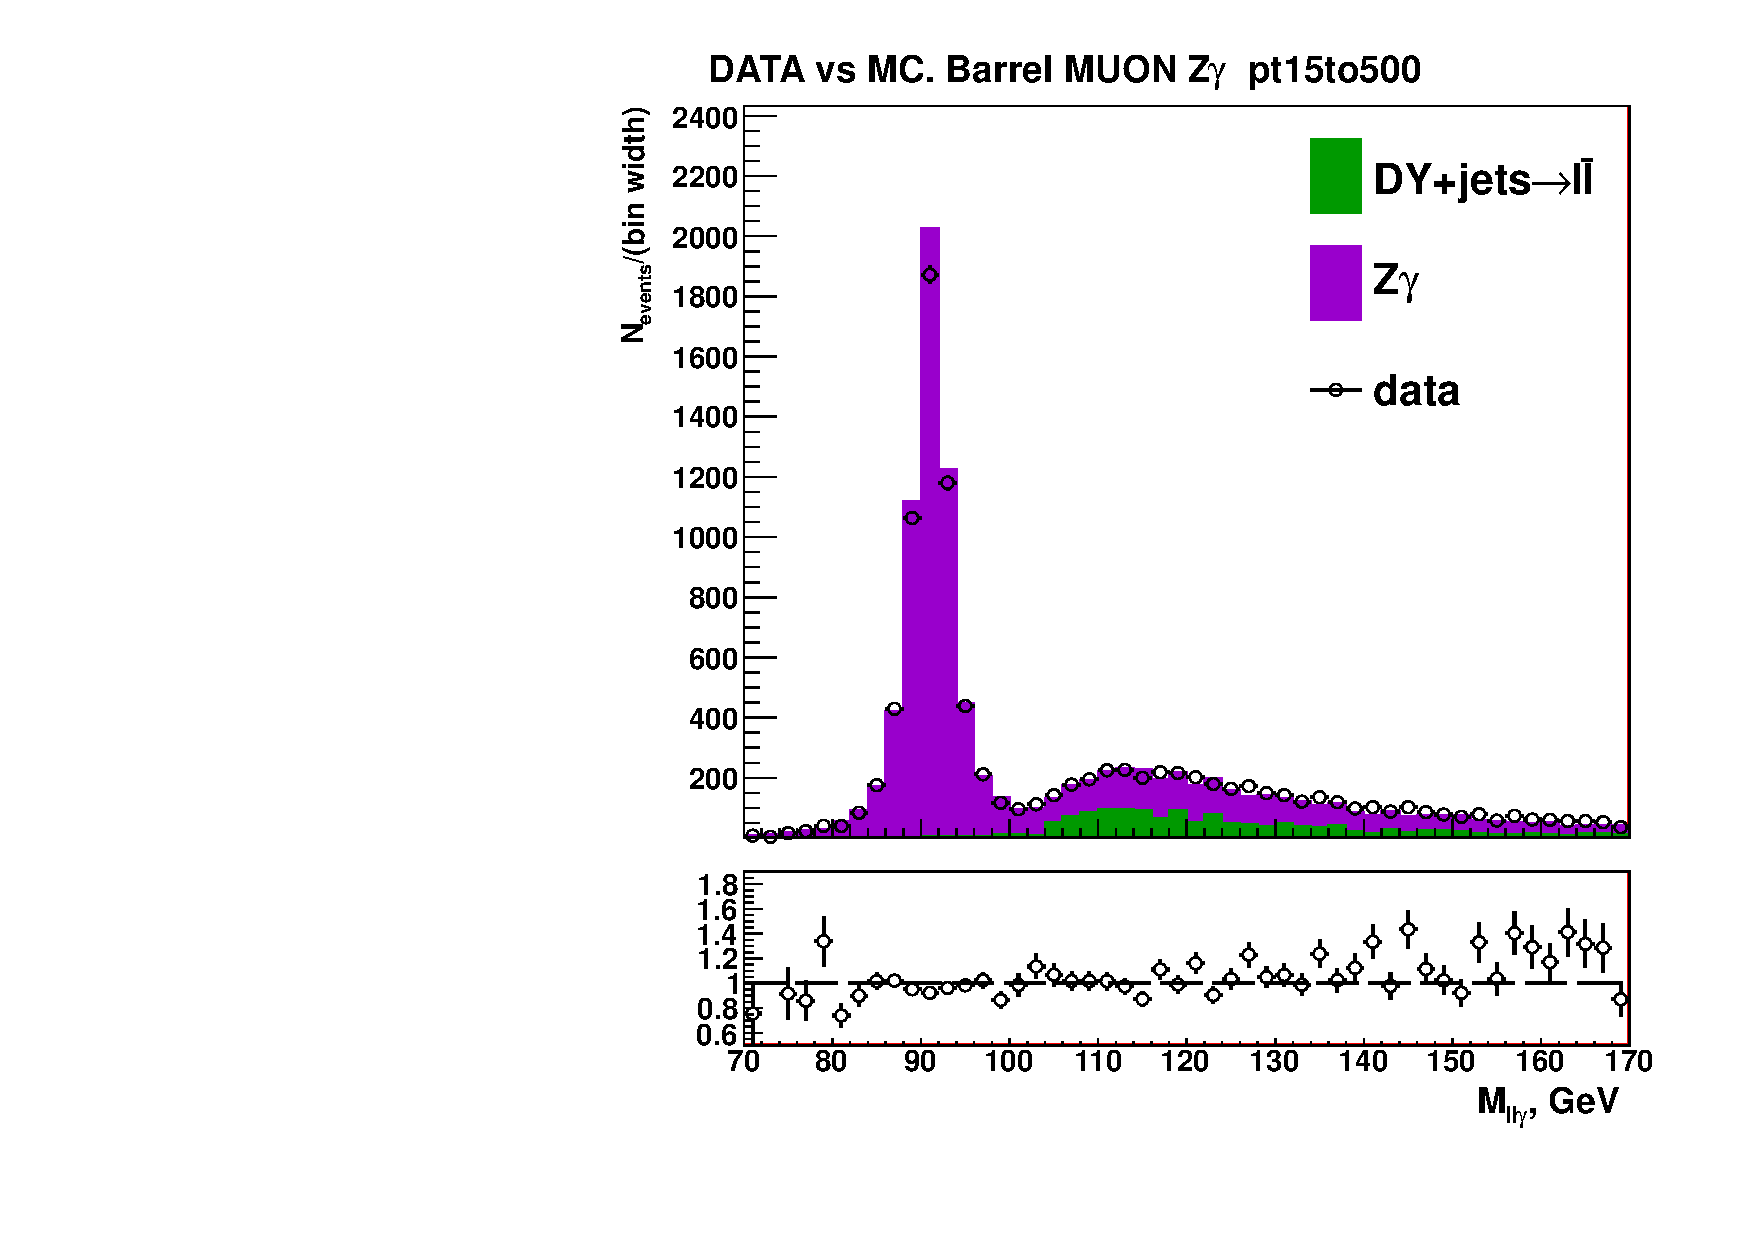
\includegraphics[width=0.45\textwidth]{../figs/figs_v11/MUON_ZGamma/PrepareYields/c_TotalDATAvsMC_Barrel__MpholeplepVERY_PRELIMINARY_pt15to500_.pdf}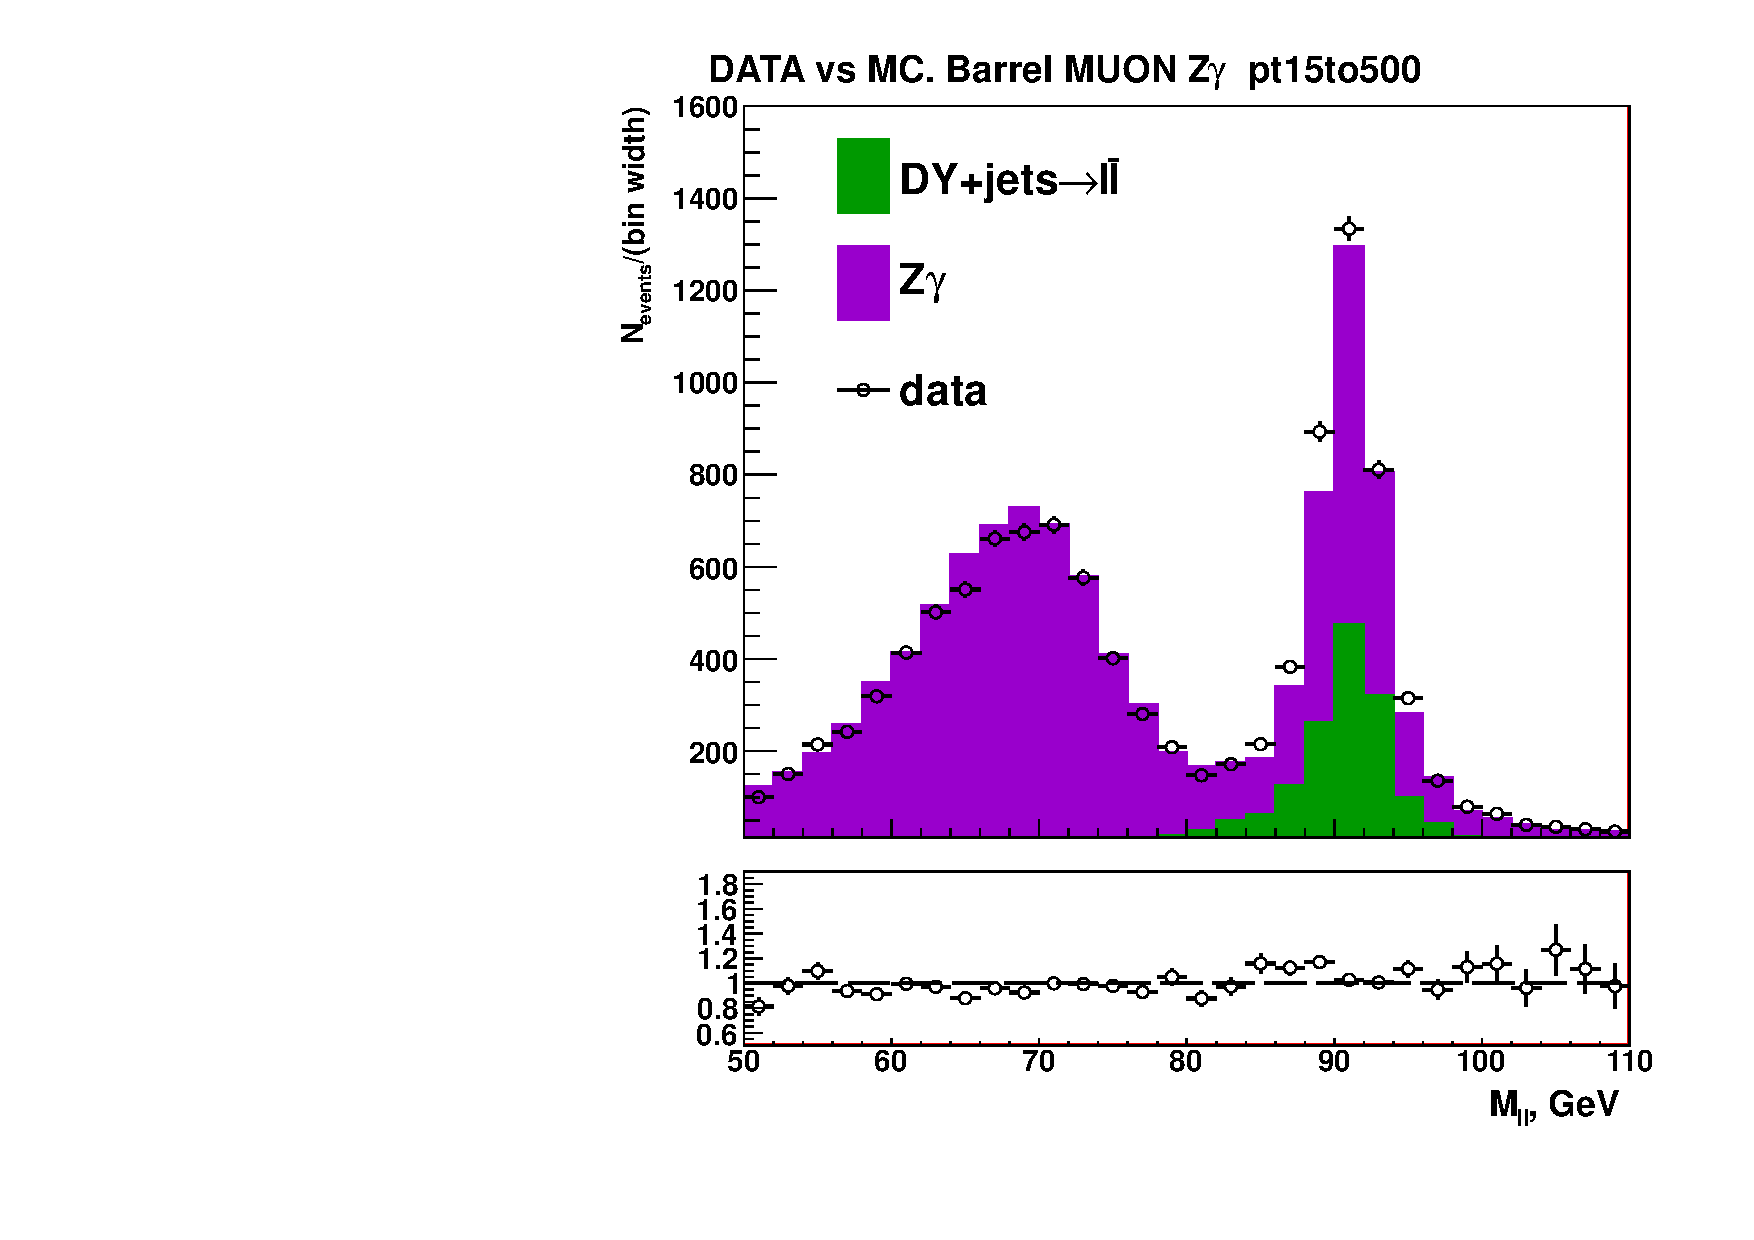
\includegraphics[width=0.45\textwidth]{../figs/figs_v11/MUON_ZGamma/PrepareYields/c_TotalDATAvsMC_Barrel__MleplepVERY_PRELIMINARY_pt15to500_.pdf}\\
   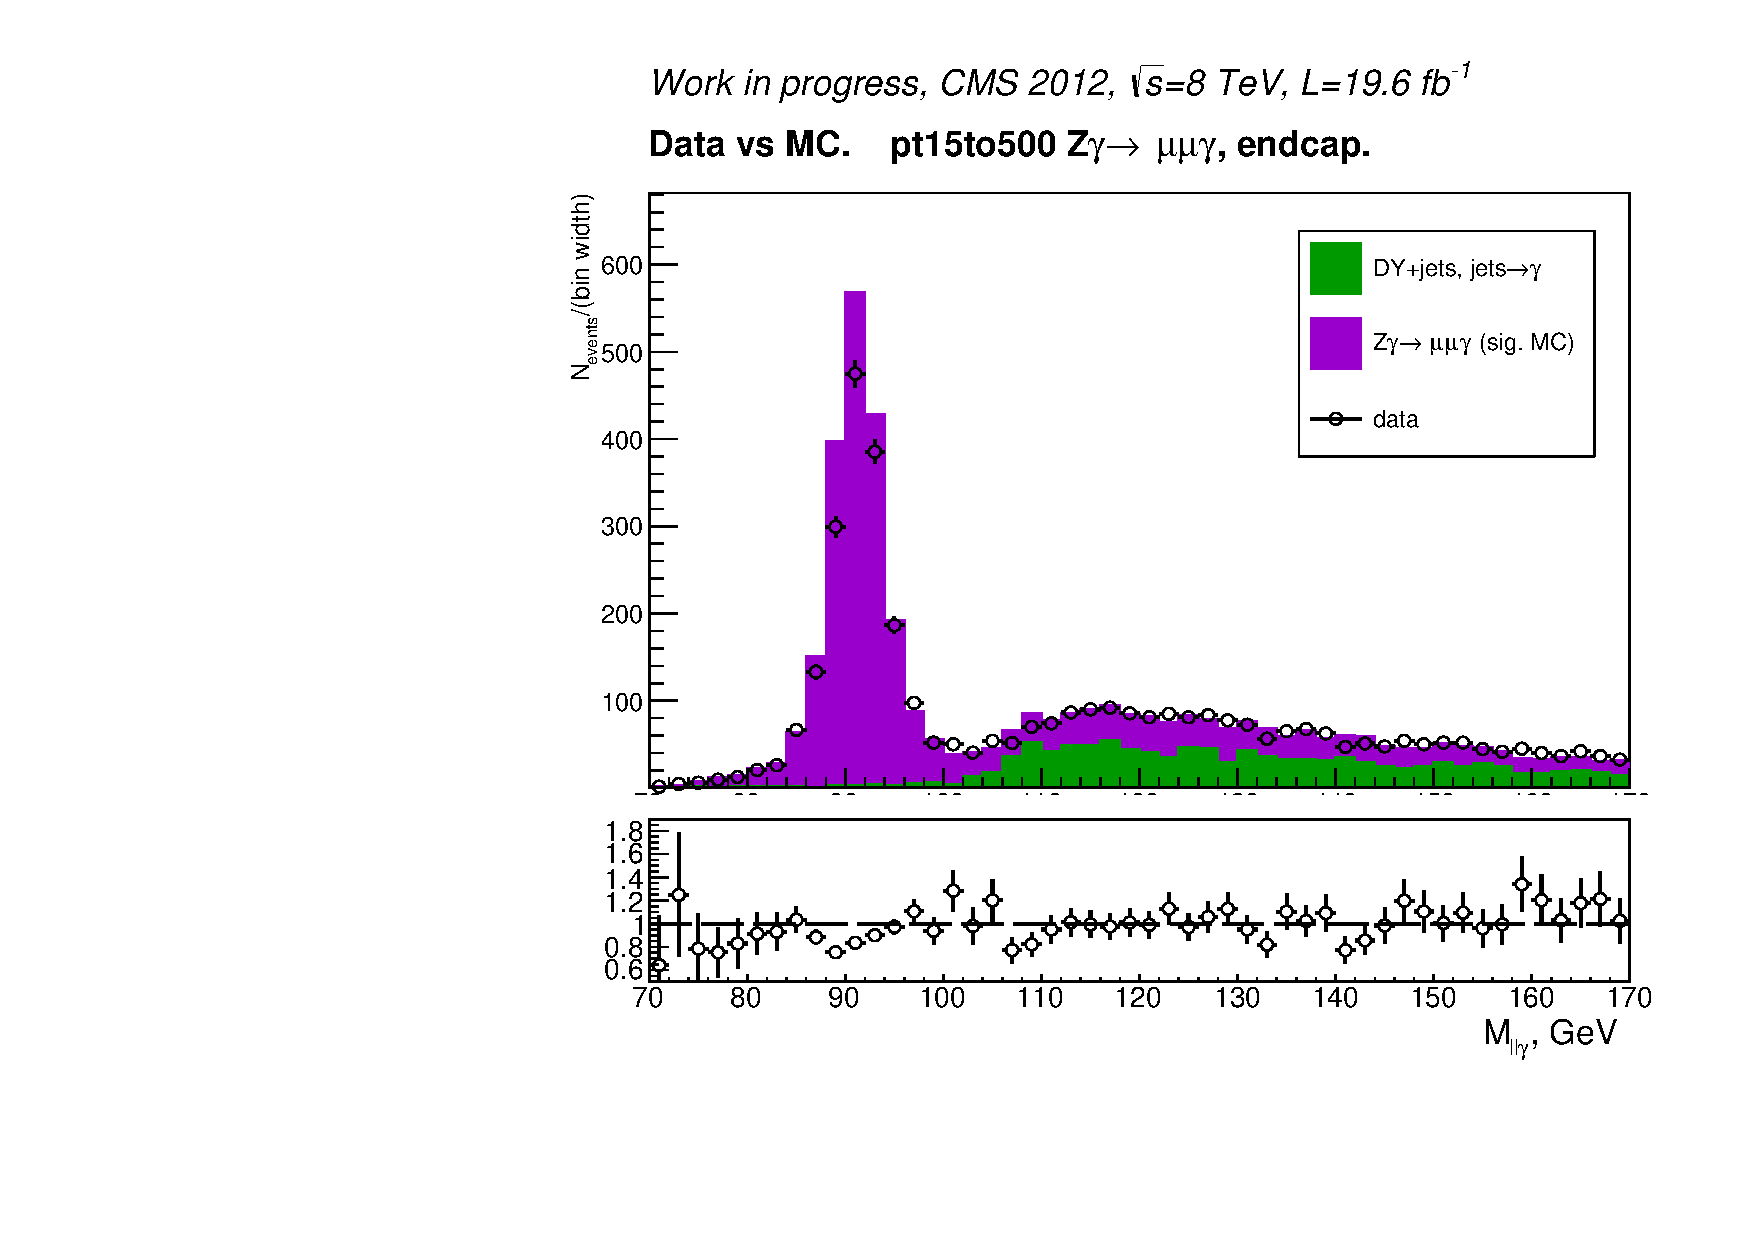
\includegraphics[width=0.45\textwidth]{../figs/figs_v11/MUON_ZGamma/PrepareYields/c_TotalDATAvsMC_Endcap__MpholeplepVERY_PRELIMINARY_pt15to500_.pdf}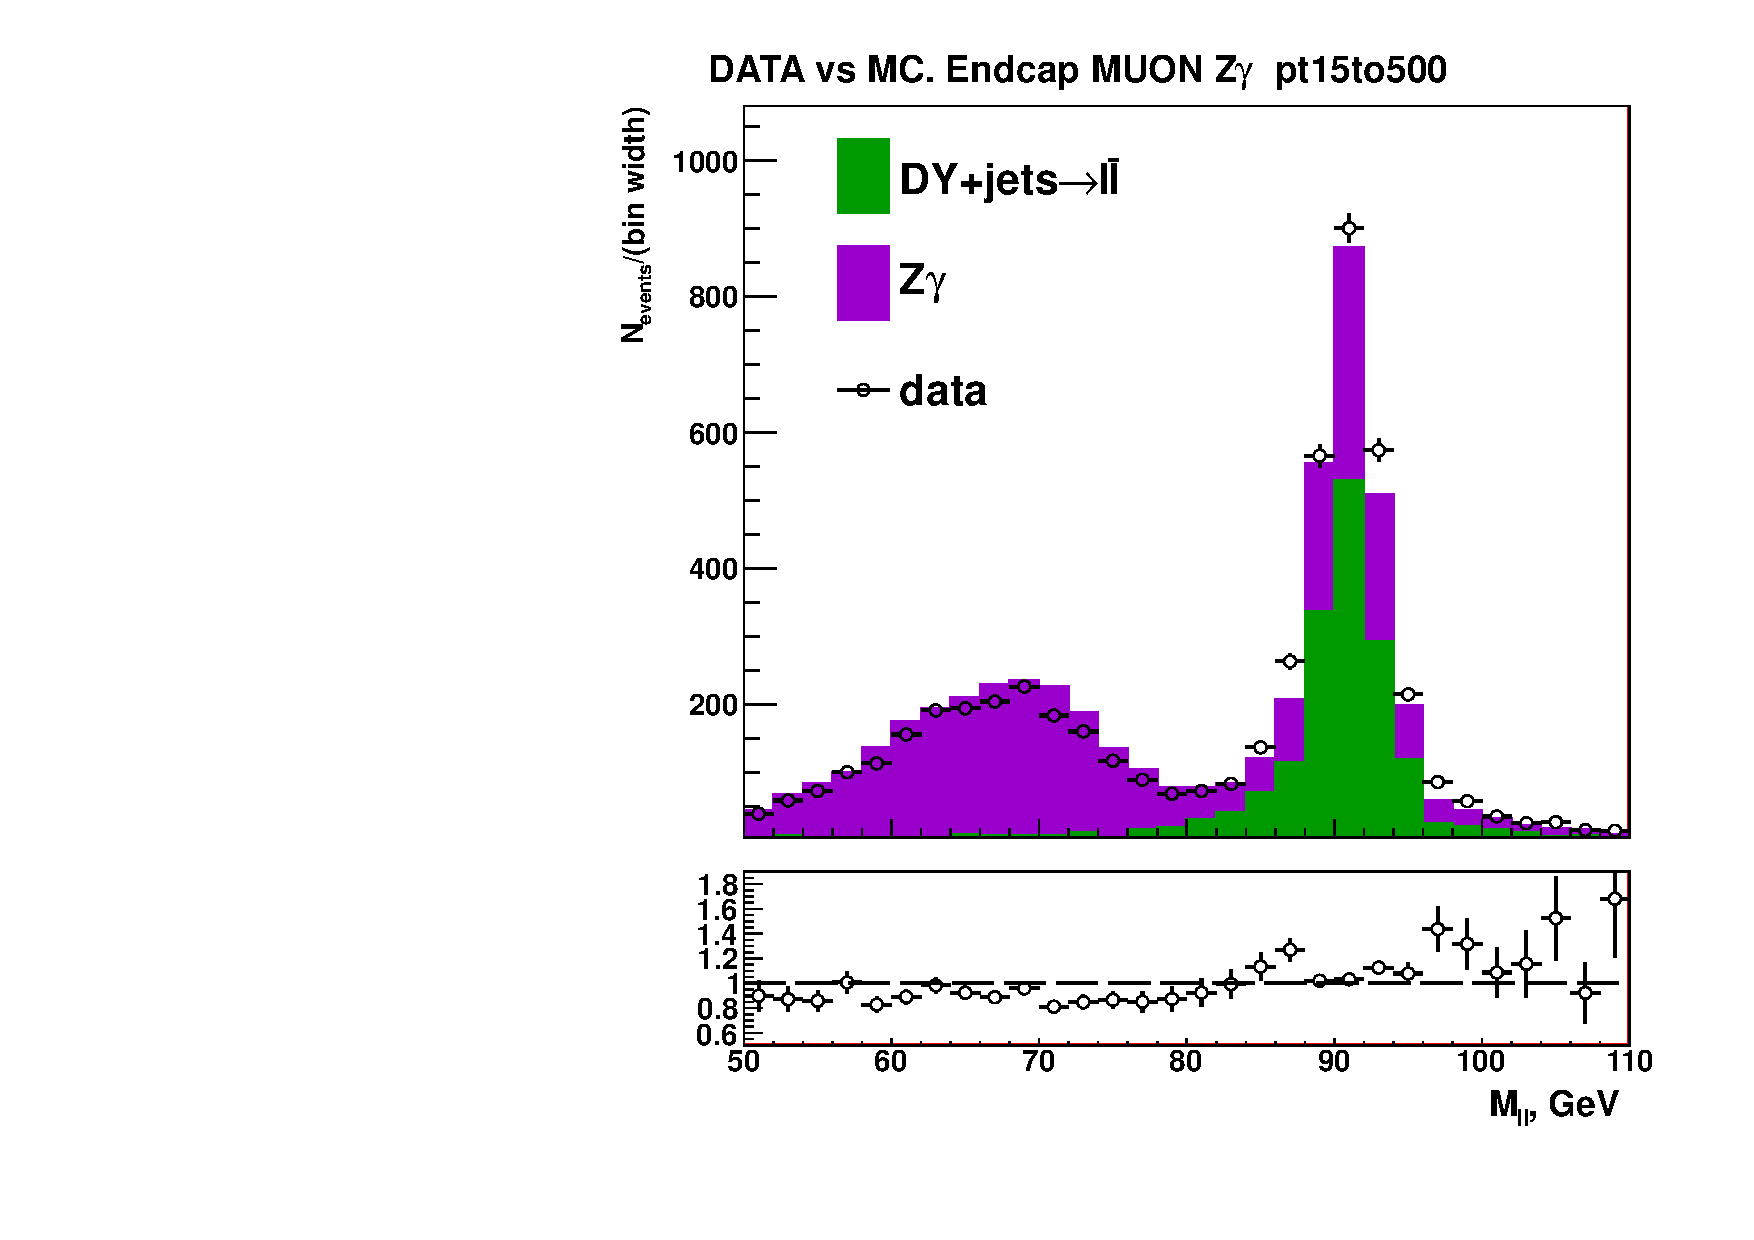
\includegraphics[width=0.45\textwidth]{../figs/figs_v11/MUON_ZGamma/PrepareYields/c_TotalDATAvsMC_Endcap__MleplepVERY_PRELIMINARY_pt15to500_.pdf}\\
  \caption{$Z\gamma$-selected events, data vs MC. Left: $M_{ll\gamma}$, right: $M_{ll}$. Top: barrel photons, bottom: endcap. Peak highly dominated by real-$\gamma$ corresponds to FSR events. FSR selection used: $81~GeV<M_{ll\gamma}<101~GeV$, $\Delta{R}(l_{1,2},\gamma)>0.4$, $\Delta{R}(l,\gamma)_{min}<1.0$, $M_{ll}<80~GeV$. ISR selection used: $80~GeV<M_{ll}<100~GeV$, $\Delta{R}(l_{1,2},\gamma)>1.0$.}
  \label{fig:Zg_Mleplep_and_Mpholeplep}
  \end{center}
\end{figure}

\begin{figure}[htb]
  \begin{center}
   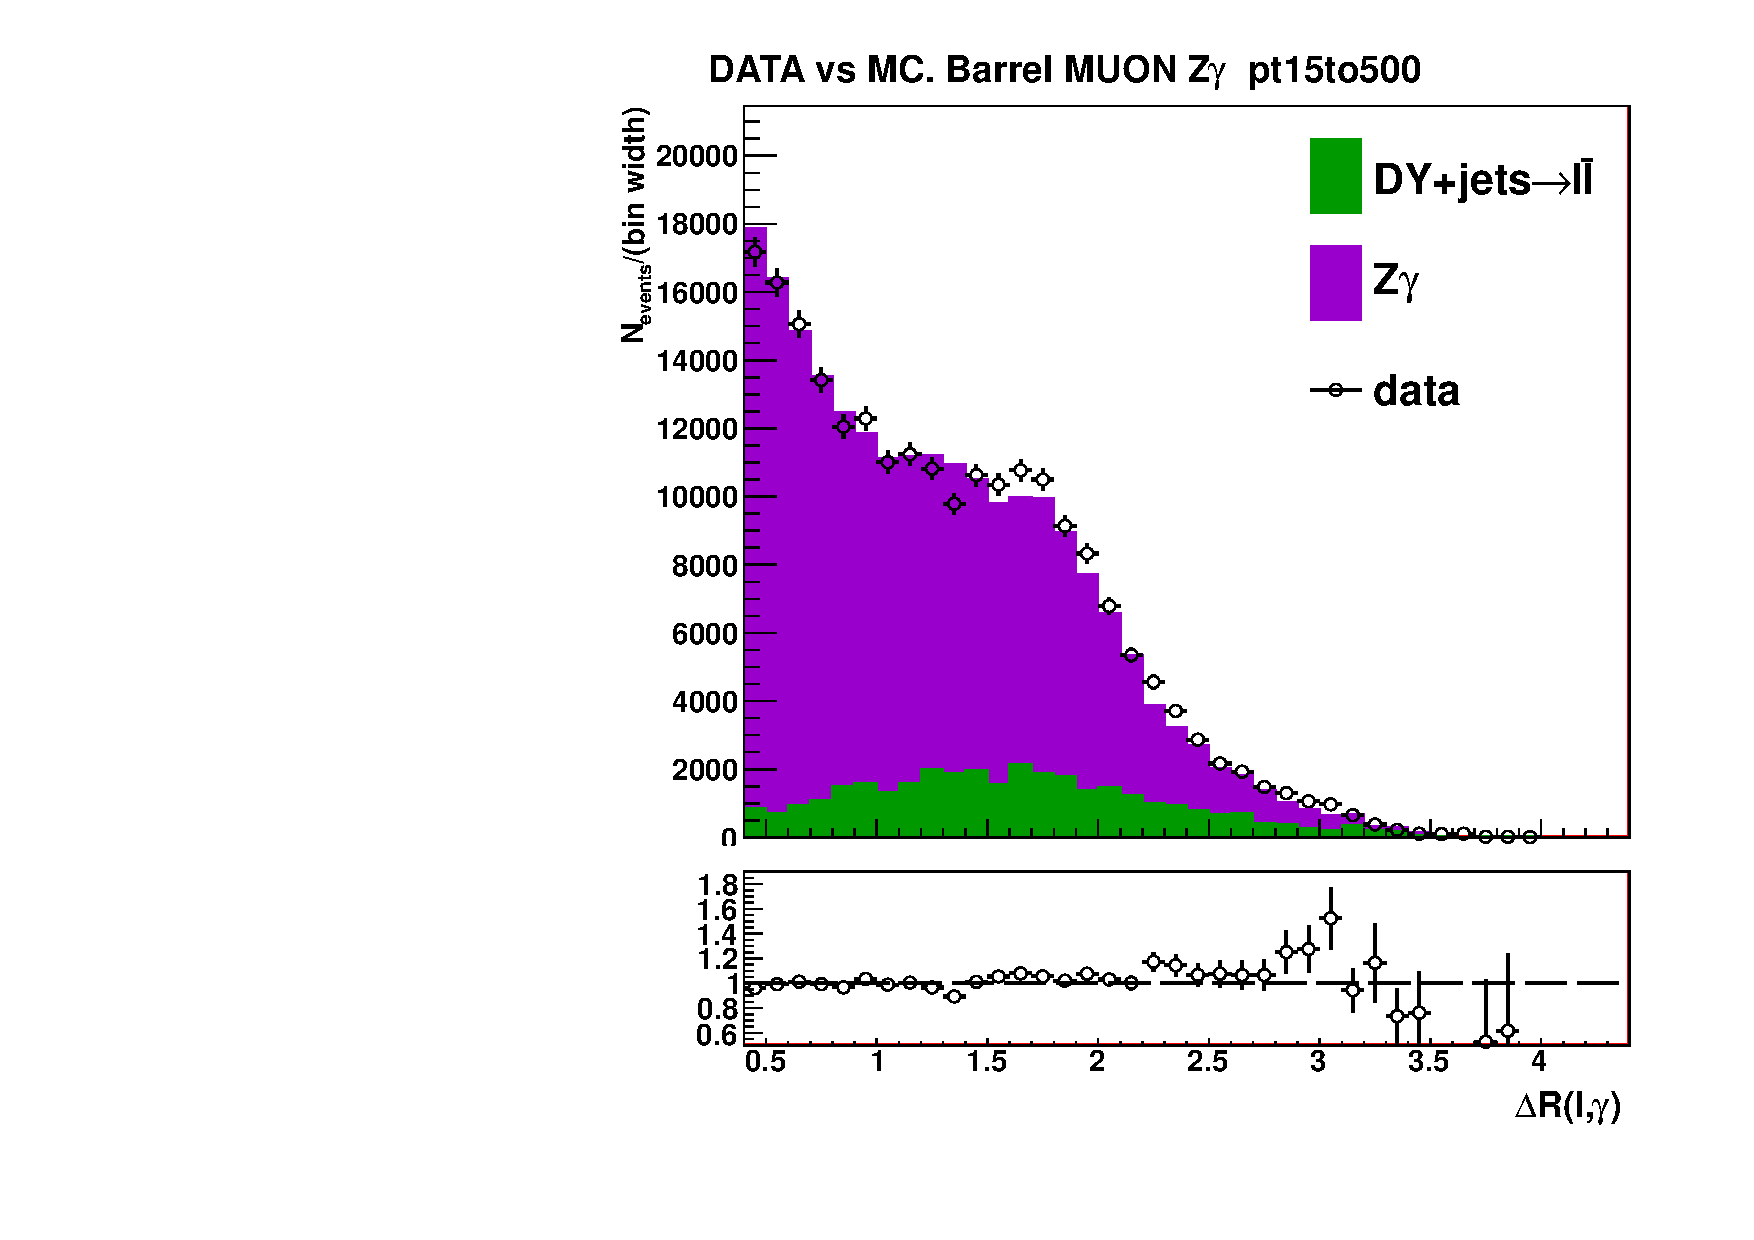
\includegraphics[width=0.45\textwidth]{../figs/figs_v11/MUON_ZGamma/PrepareYields/c_TotalDATAvsMC_Barrel__lep1PhoDeltaRVERY_PRELIMINARY_pt15to500_.pdf}   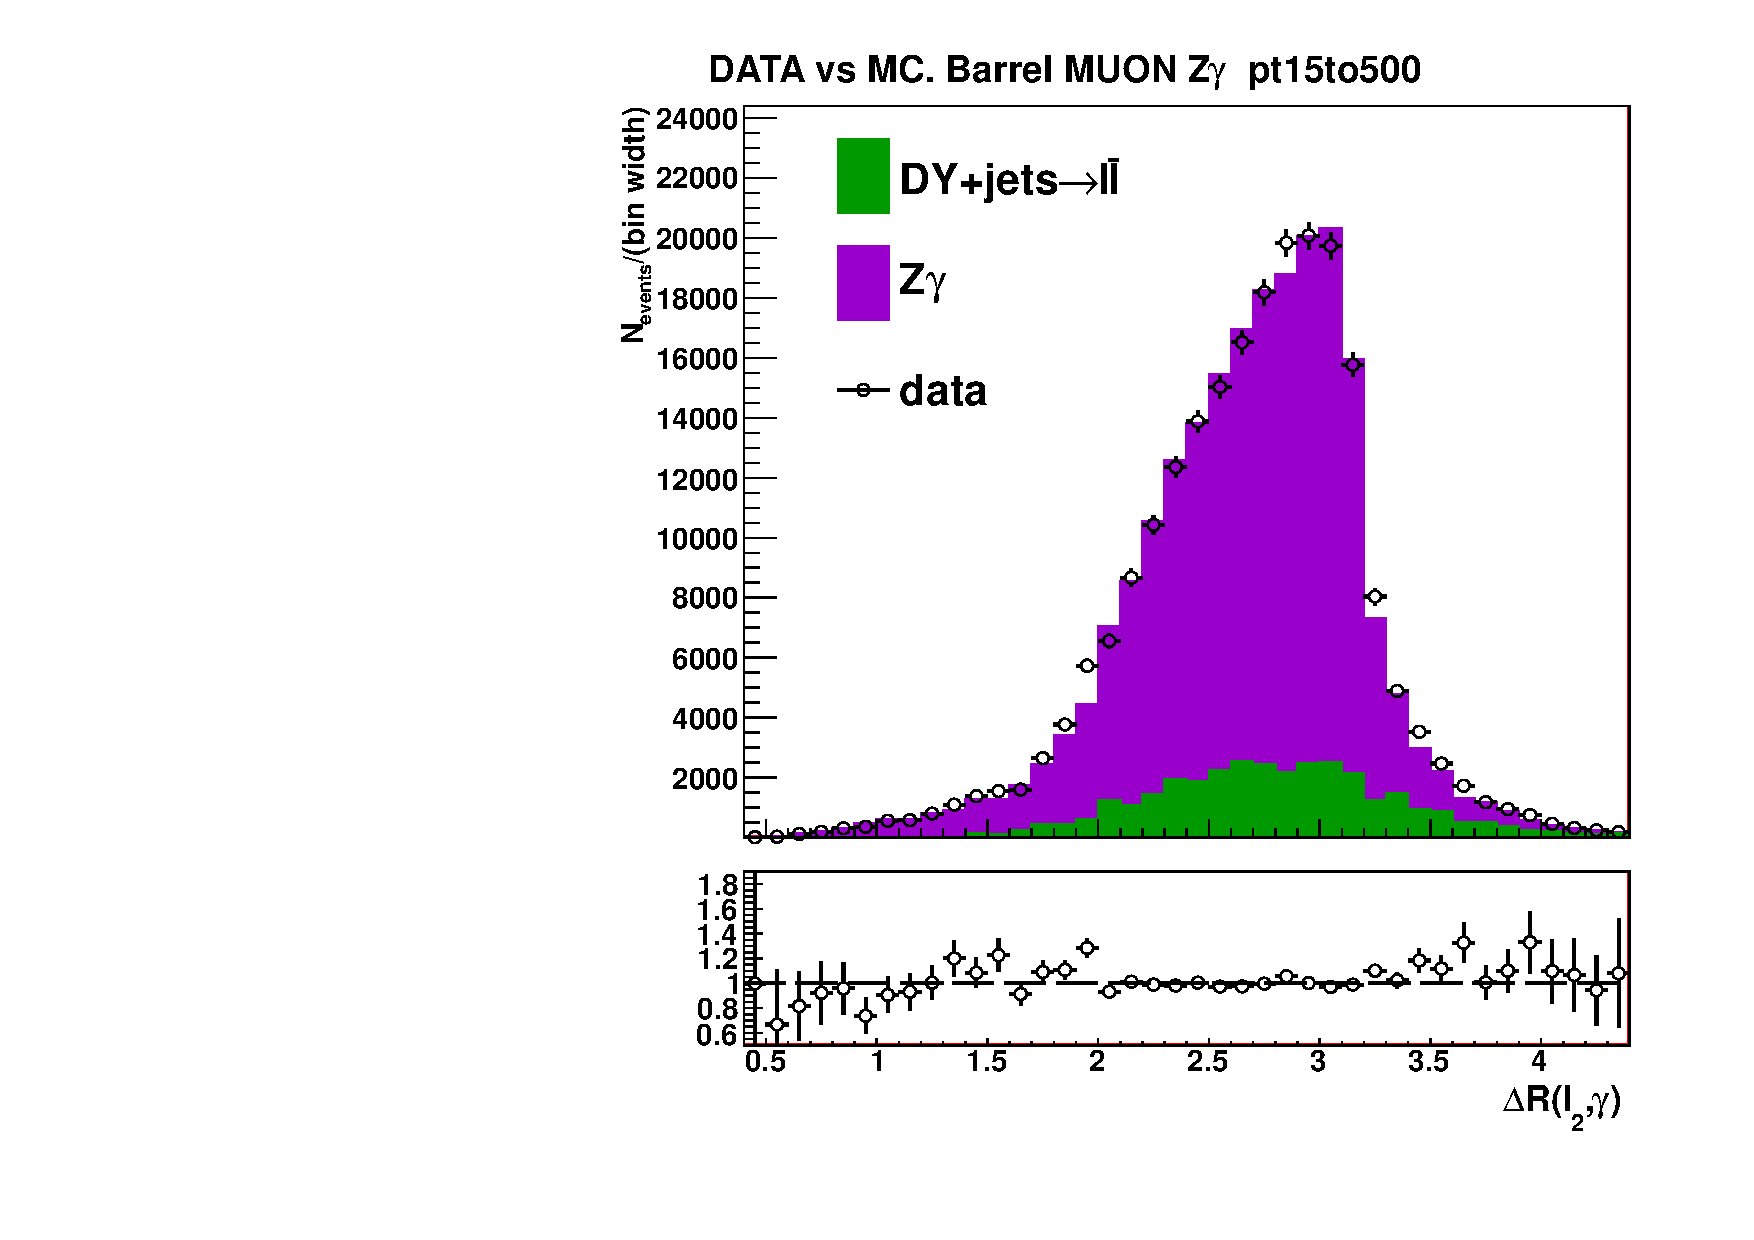
\includegraphics[width=0.45\textwidth]{../figs/figs_v11/MUON_ZGamma/PrepareYields/c_TotalDATAvsMC_Barrel__lep2PhoDeltaRVERY_PRELIMINARY_pt15to500_.pdf}\\
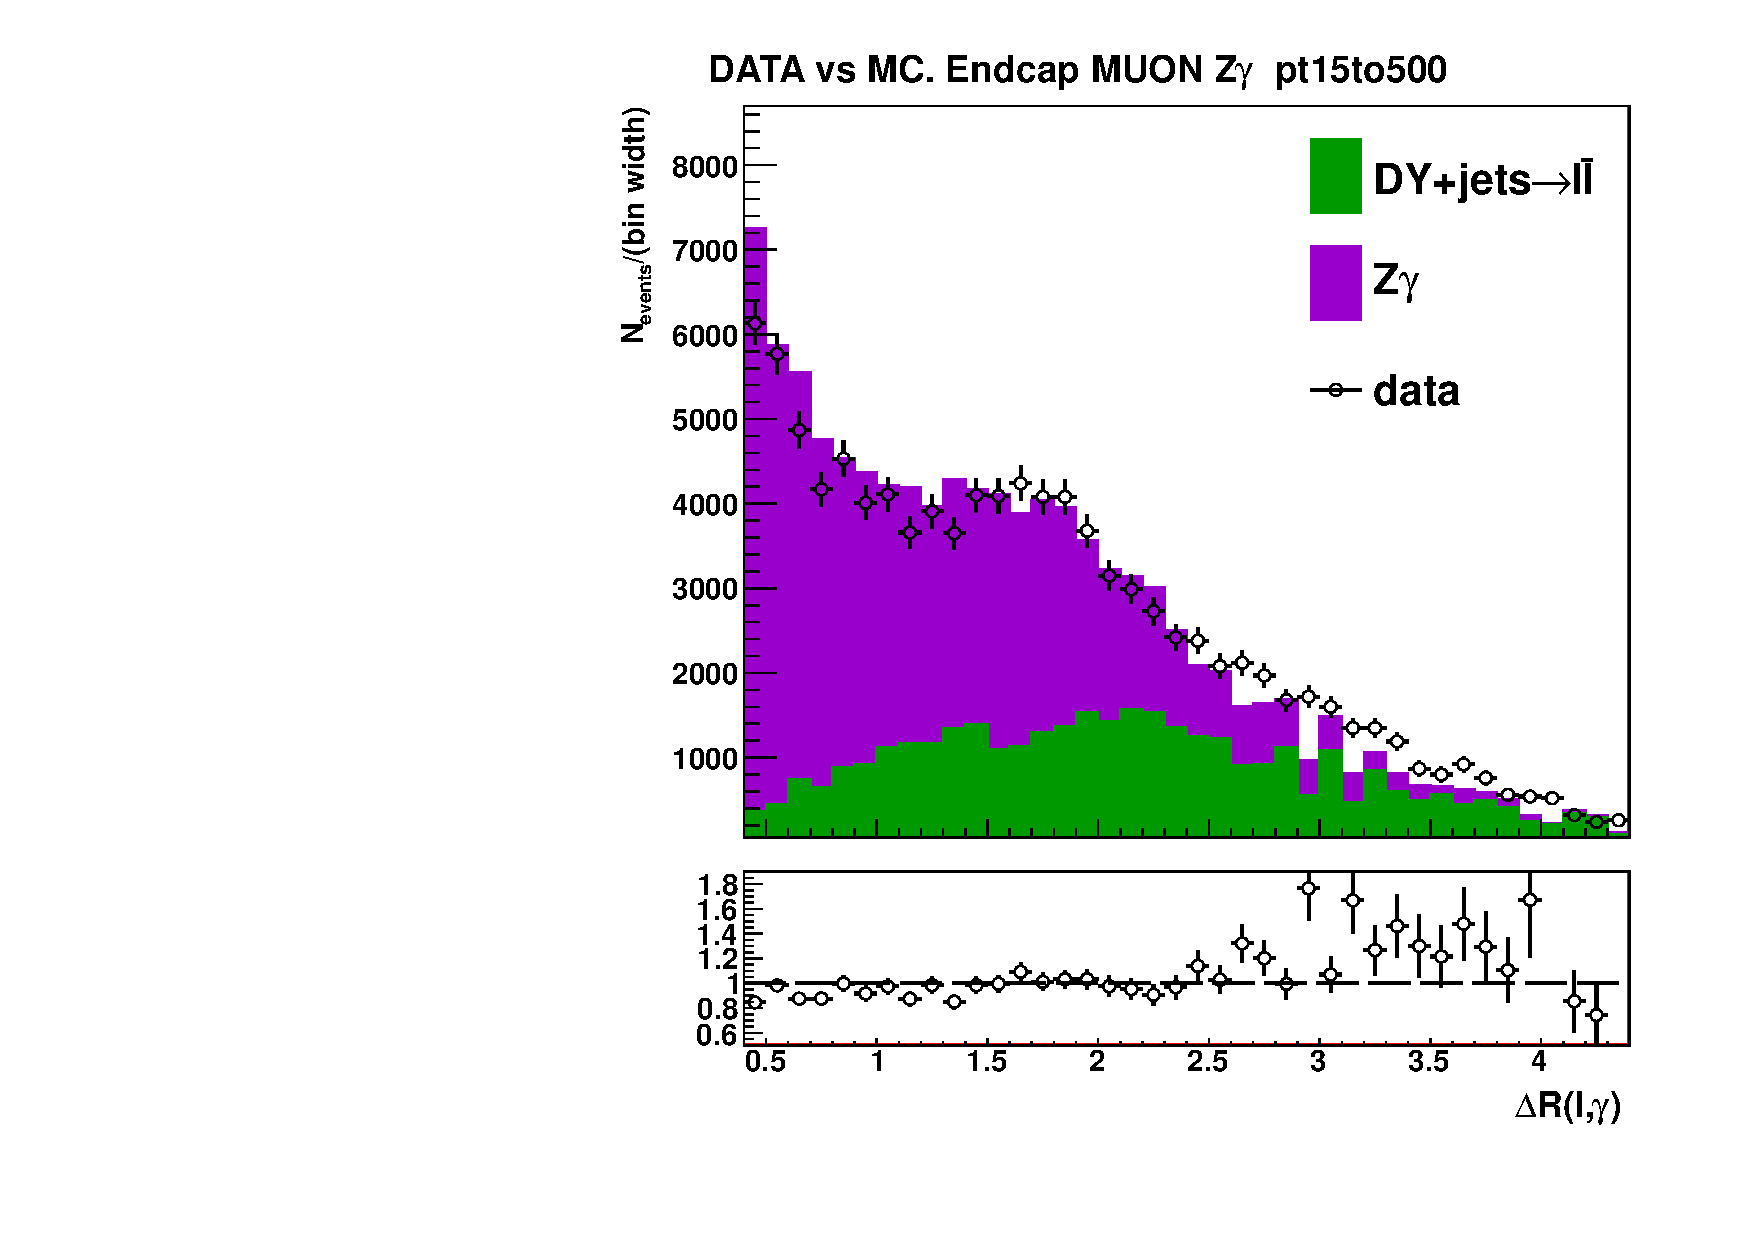
\includegraphics[width=0.45\textwidth]{../figs/figs_v11/MUON_ZGamma/PrepareYields/c_TotalDATAvsMC_Endcap__lep1PhoDeltaRVERY_PRELIMINARY_pt15to500_.pdf}   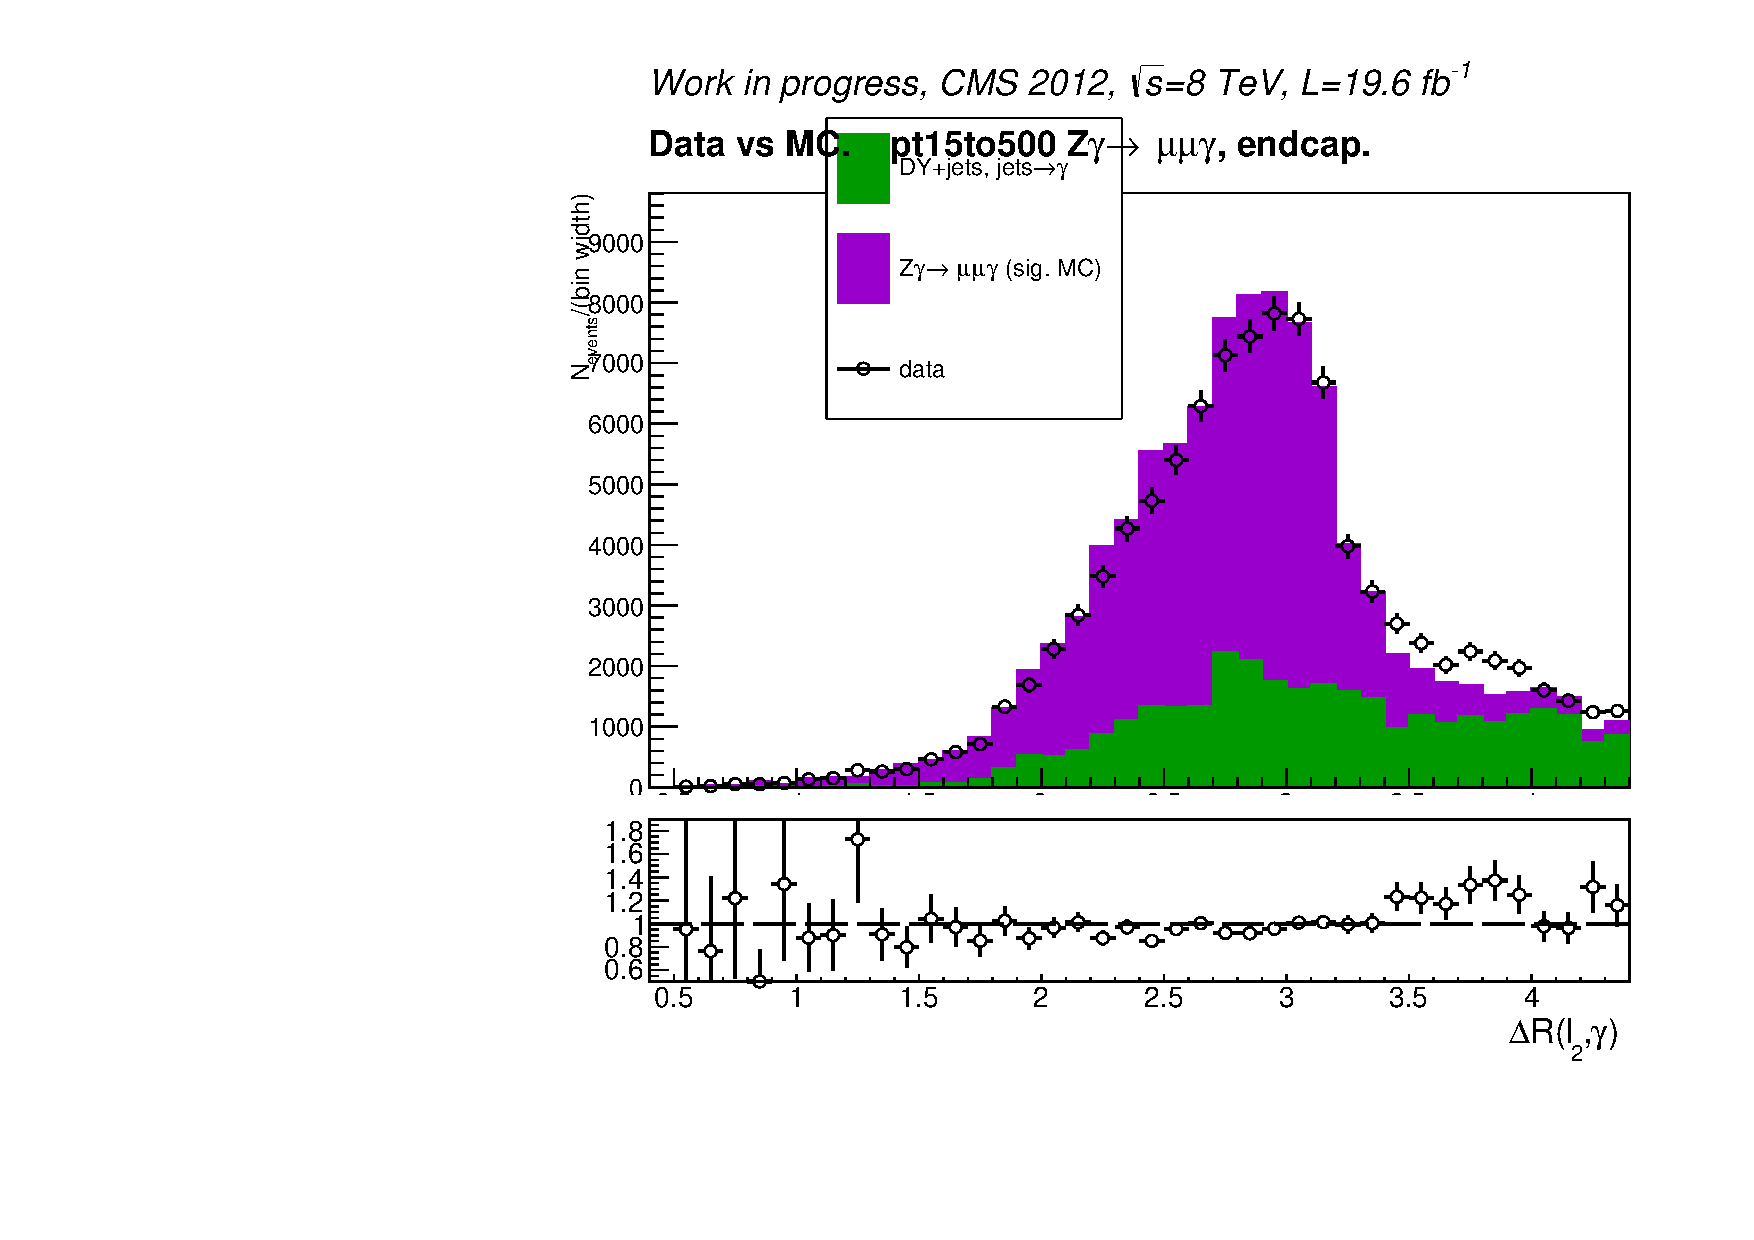
\includegraphics[width=0.45\textwidth]{../figs/figs_v11/MUON_ZGamma/PrepareYields/c_TotalDATAvsMC_Endcap__lep2PhoDeltaRVERY_PRELIMINARY_pt15to500_.pdf}    \\
  \caption{$Z\gamma$-selected FSR (top) and ISR (bottom) events, data vs MC. FSR selection used: $81~GeV<M_{ll\gamma}<101~GeV$, $\Delta{R}(l_{1,2},\gamma)>0.4$, $\Delta{R}(l,\gamma)_{min}<1.0$, $M_{ll}<80~GeV$. ISR selection used: $80~GeV<M_{ll}<100~GeV$, $\Delta{R}(l_{1,2},\gamma)>1.0$.}
  \label{fig:Zg_ISRandFSR_dR}
  \end{center}
\end{figure}

\begin{figure}[htb]
  \begin{center}
   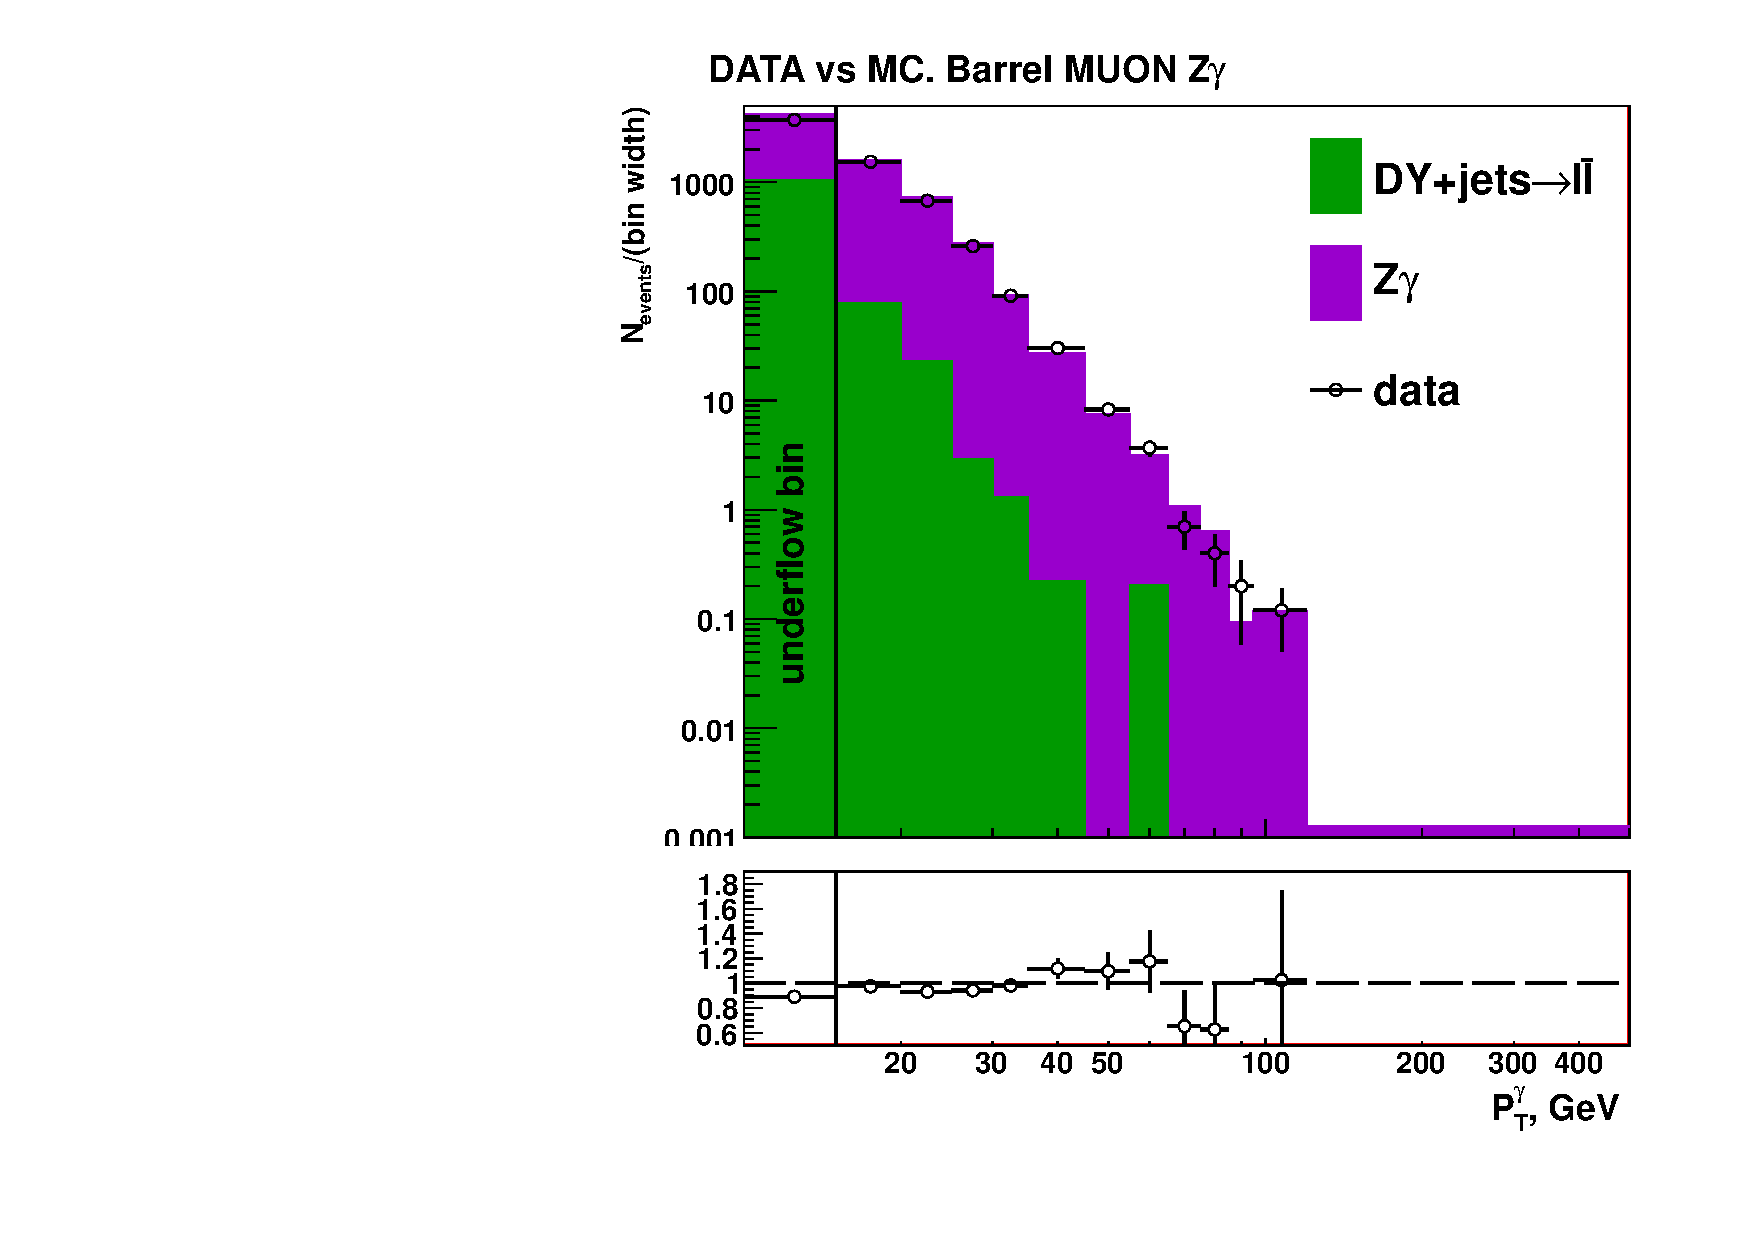
\includegraphics[width=0.45\textwidth]{../figs/figs_v11/MUON_ZGamma/PrepareYields/c_TotalDATAvsMC_Barrel__phoEtFSR.pdf}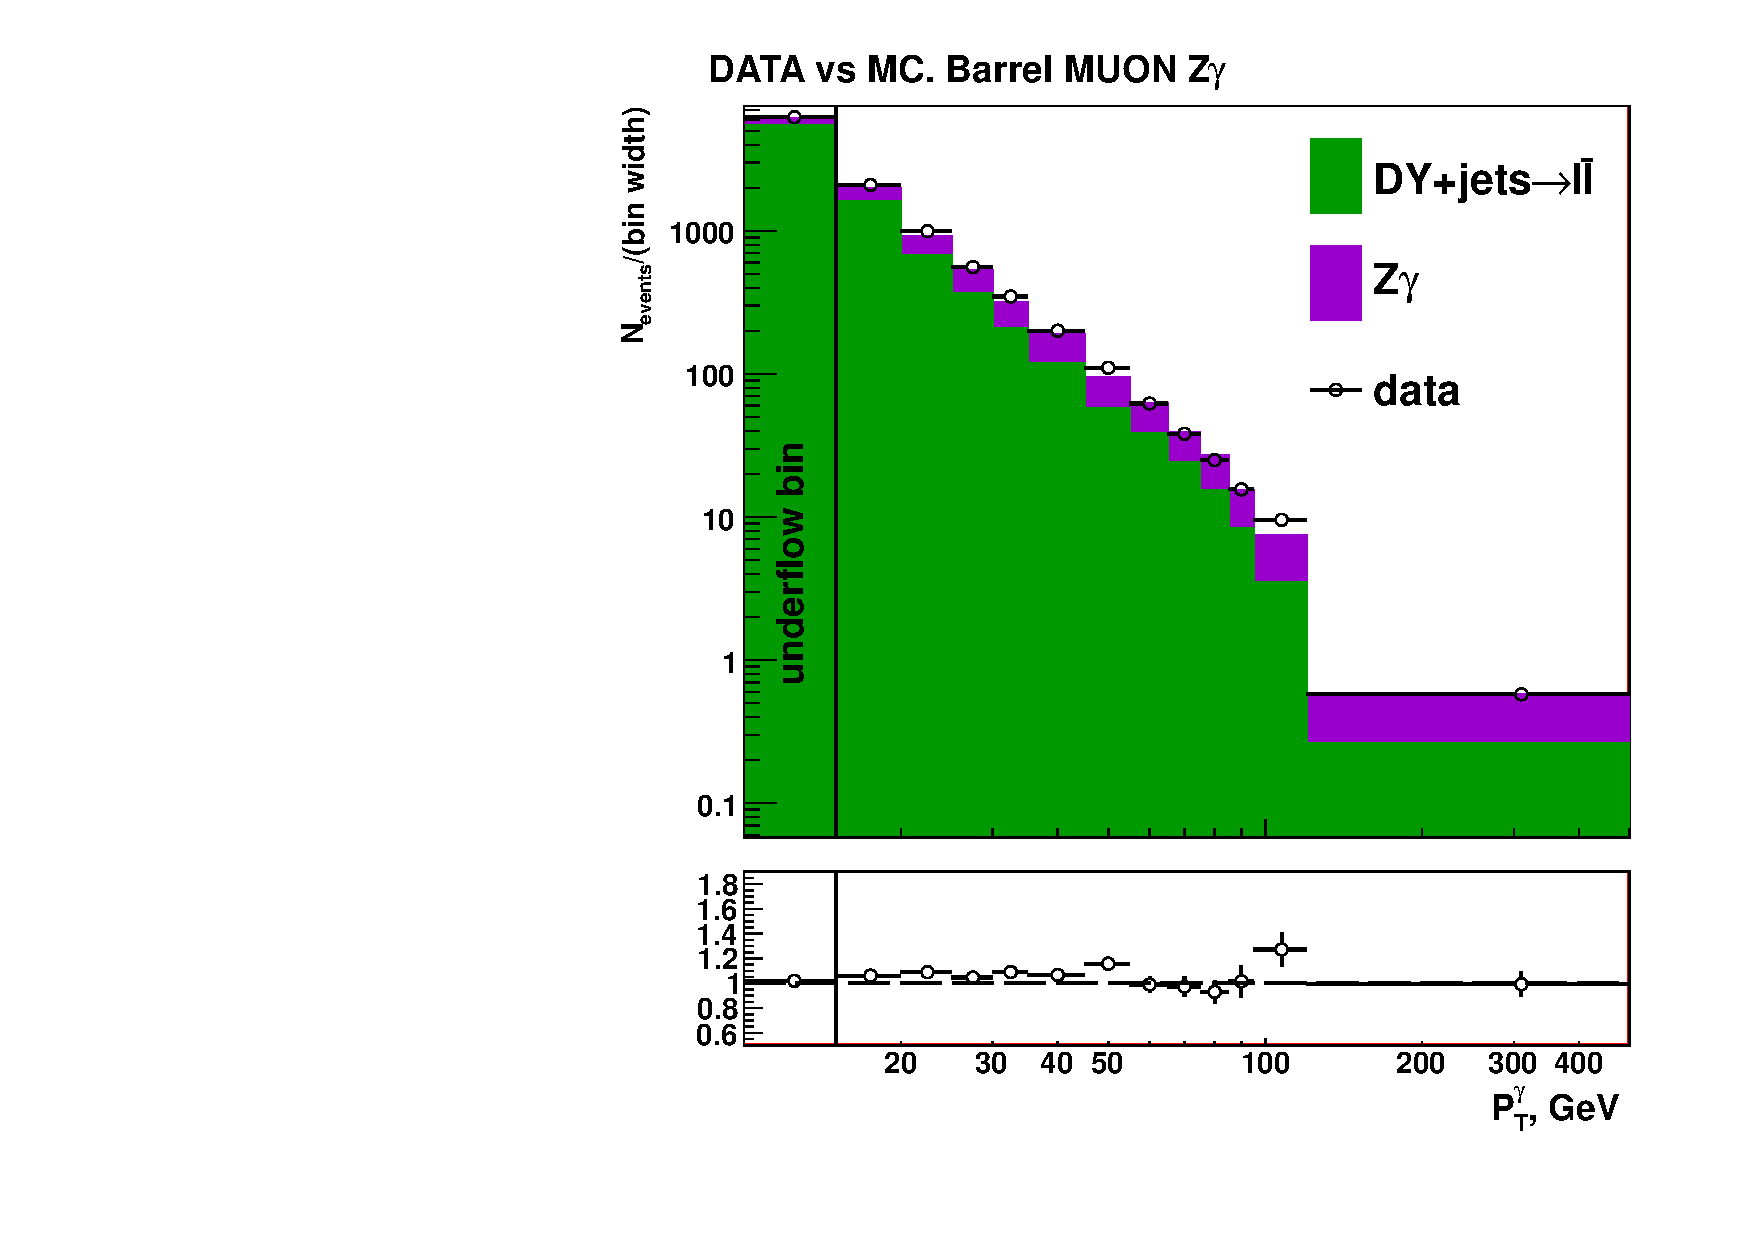
\includegraphics[width=0.45\textwidth]{../figs/figs_v11/MUON_ZGamma/PrepareYields/c_TotalDATAvsMC_Barrel__phoEtFSR_EXCLUDED.pdf}\\
   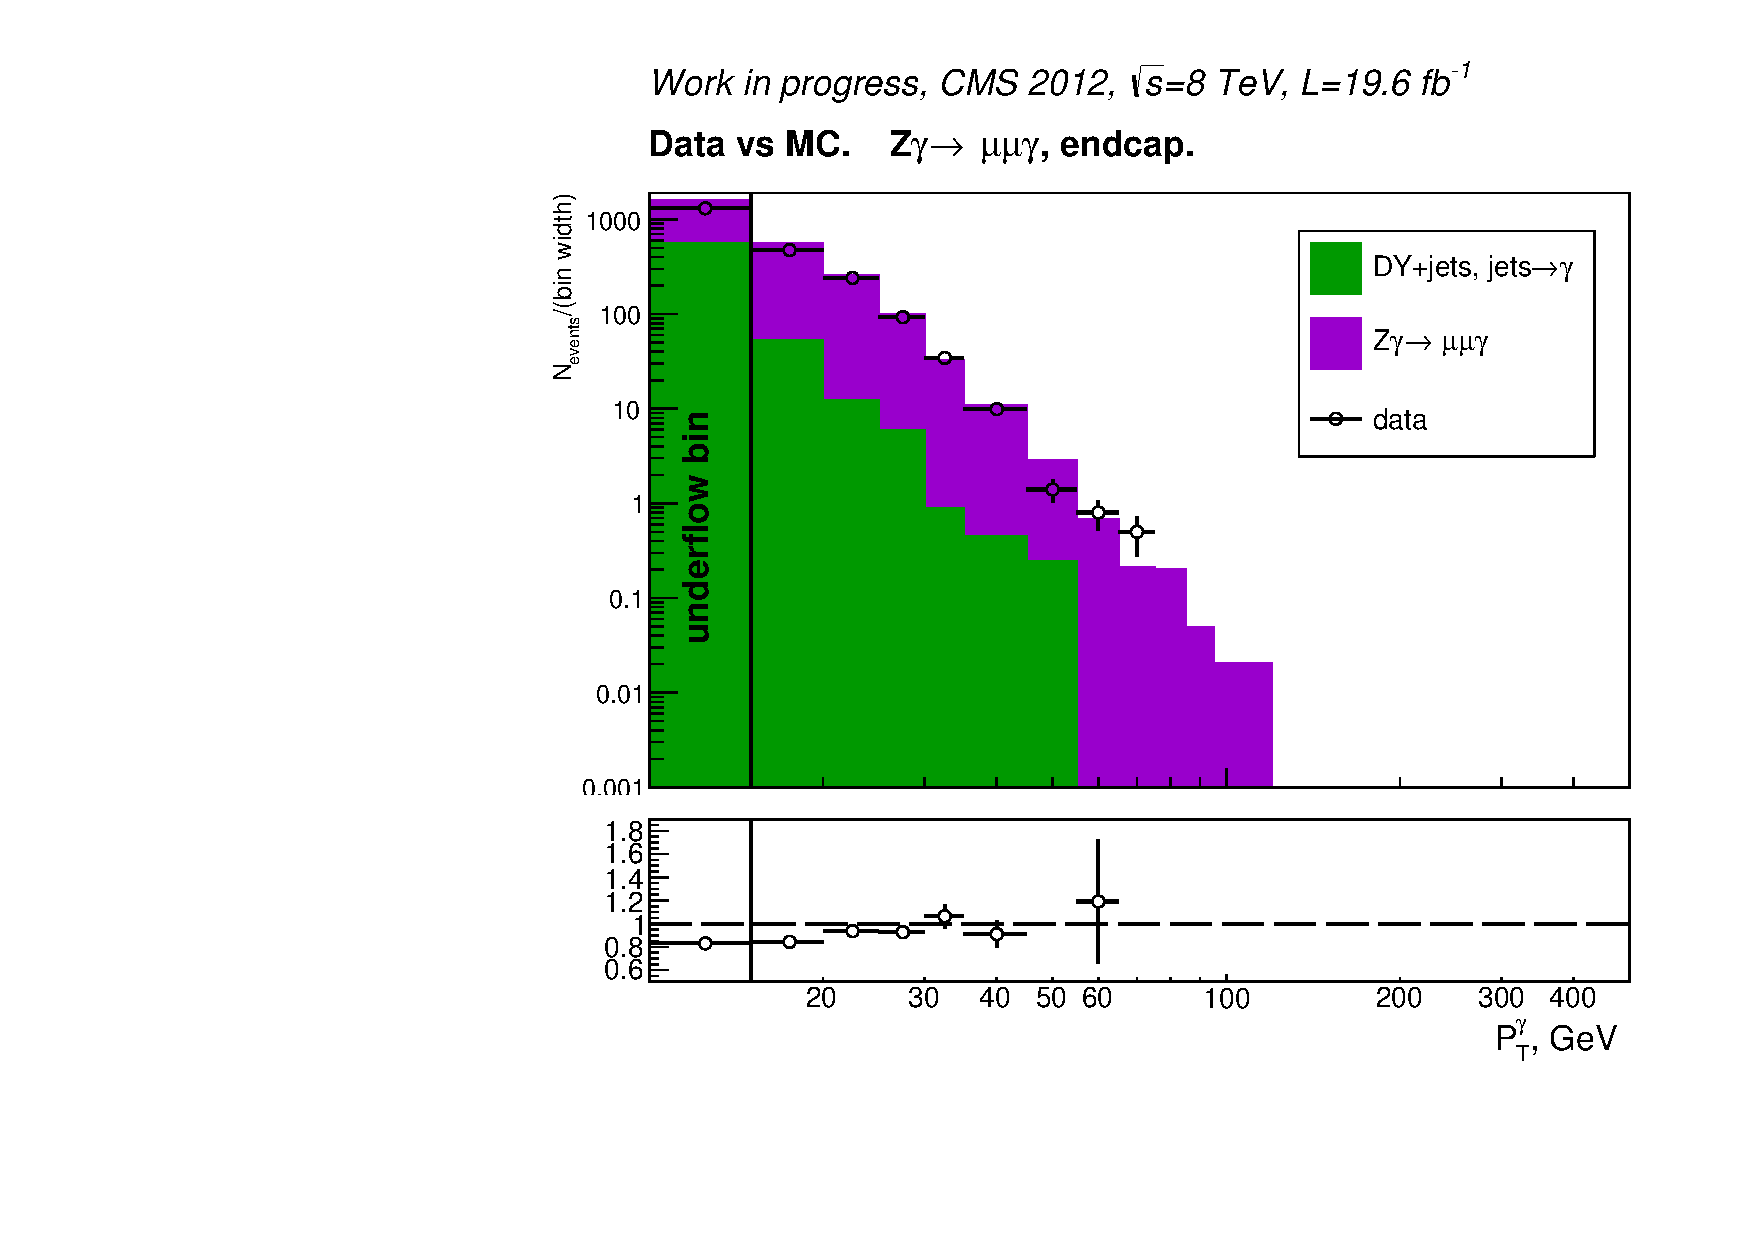
\includegraphics[width=0.45\textwidth]{../figs/figs_v11/MUON_ZGamma/PrepareYields/c_TotalDATAvsMC_Endcap__phoEtFSR.pdf}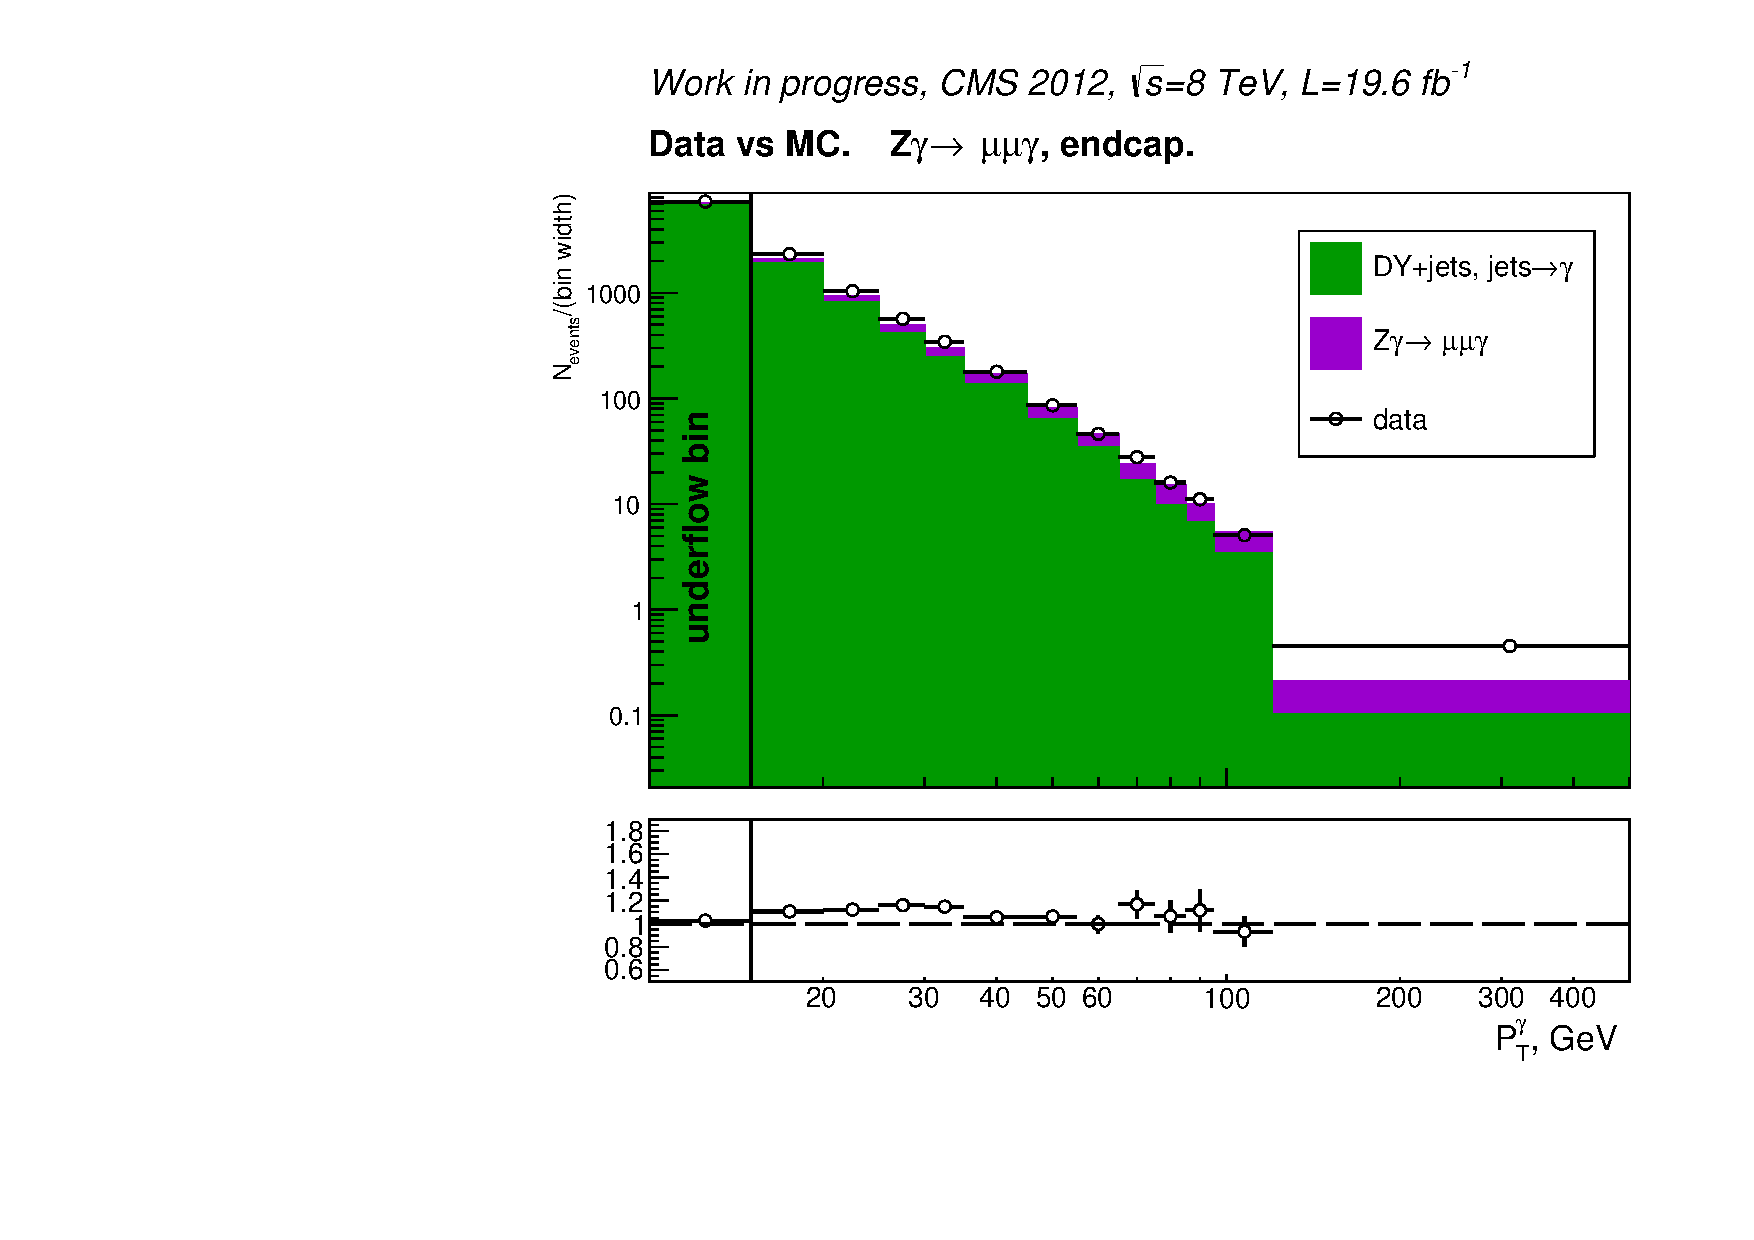
\includegraphics[width=0.45\textwidth]{../figs/figs_v11/MUON_ZGamma/PrepareYields/c_TotalDATAvsMC_Endcap__phoEtFSR_EXCLUDED.pdf}\\
  \caption{$Z\gamma$-selected FSR (left) and ISR (right) events, data vs MC. FSR selection used: $81~GeV<M_{ll\gamma}<101~GeV$, $\Delta{R}(l_{1,2},\gamma)>0.4$, $\Delta{R}(l,\gamma)_{min}<1.0$, $M_{ll}<80~GeV$. ISR selection used: $80~GeV<M_{ll}<100~GeV$, $\Delta{R}(l_{1,2},\gamma)>1.0$.}
  \label{fig:Zg_ISRandFSR_phoEt}
  \end{center}
\end{figure}

\begin{figure}[htb]
  \begin{center}
   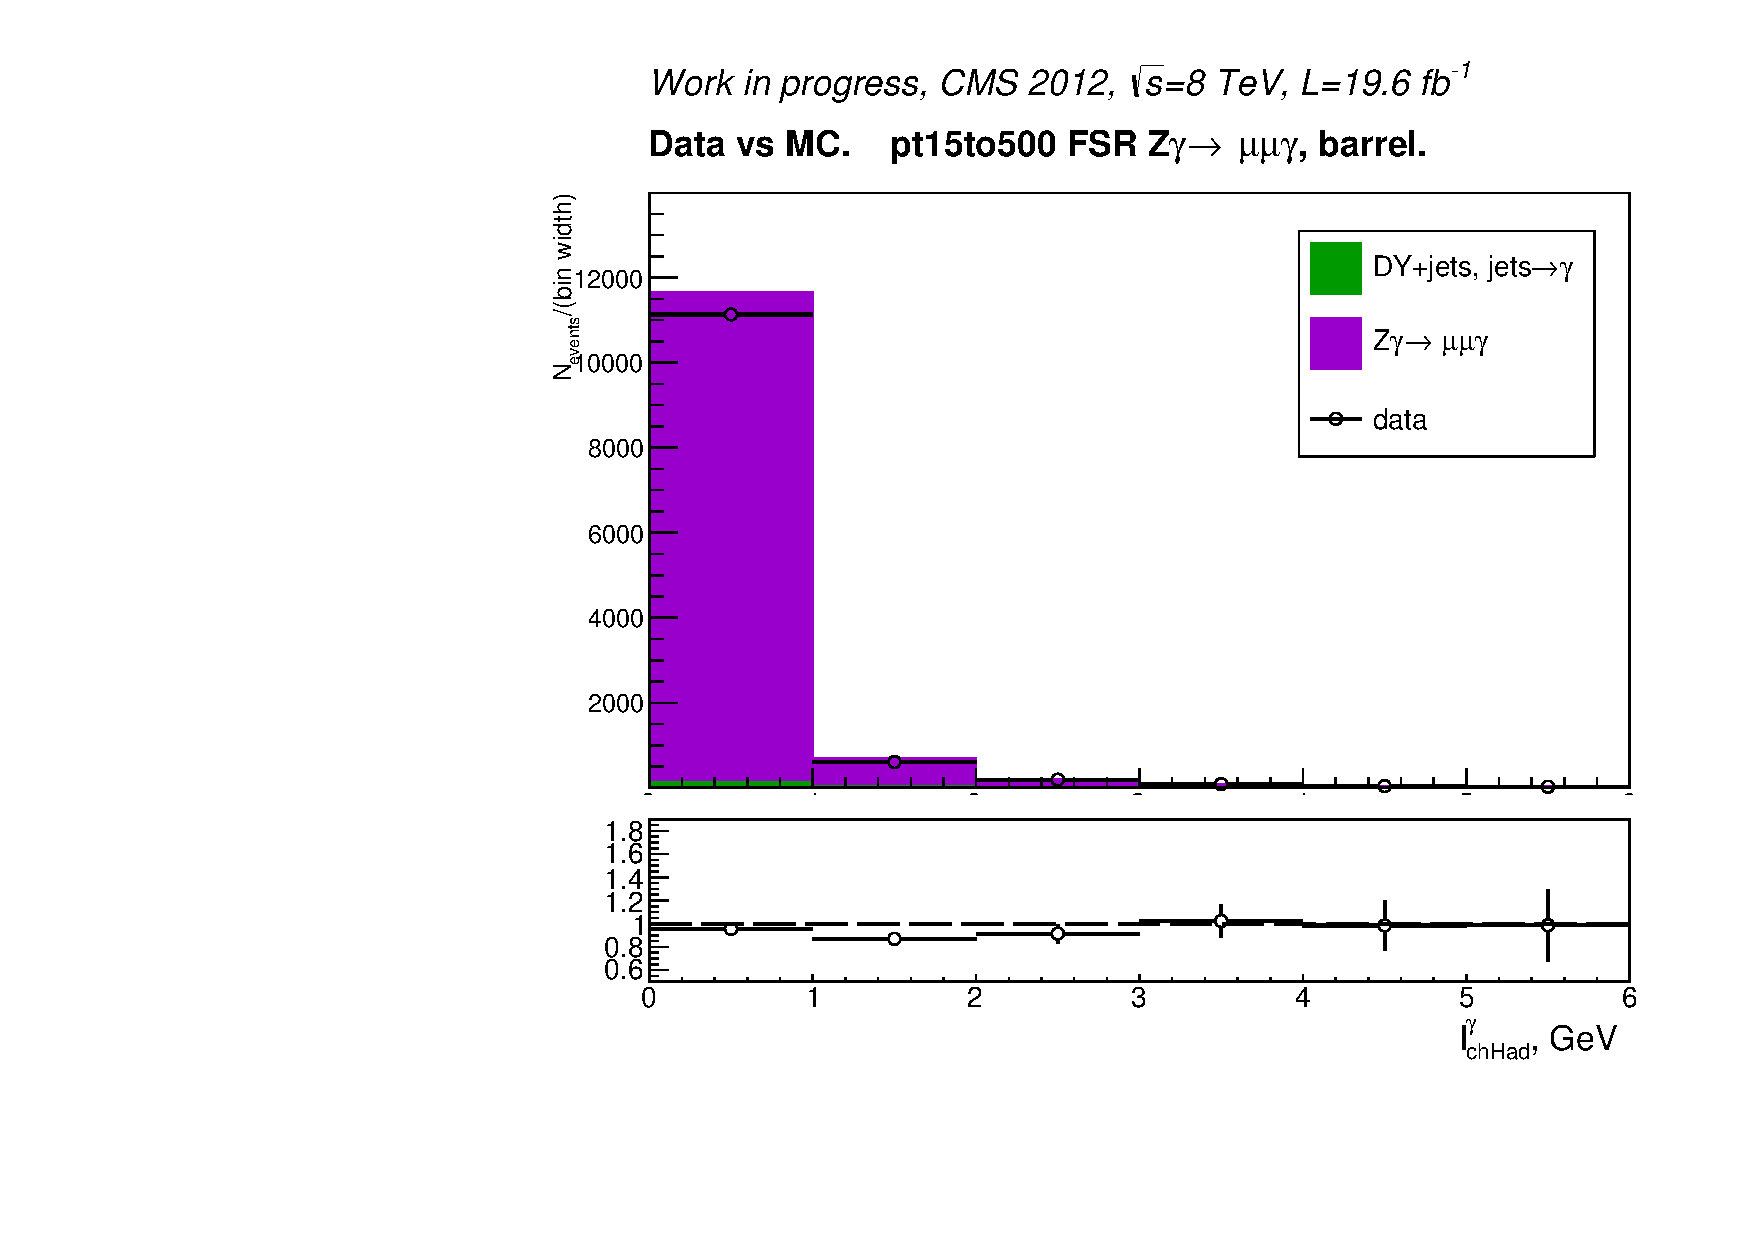
\includegraphics[width=0.45\textwidth]{../figs/figs_v11/MUON_ZGamma/PrepareYields/c_TotalDATAvsMC_Barrel__phoPFChIsoCorrFSR_pt15to500_FSR.pdf}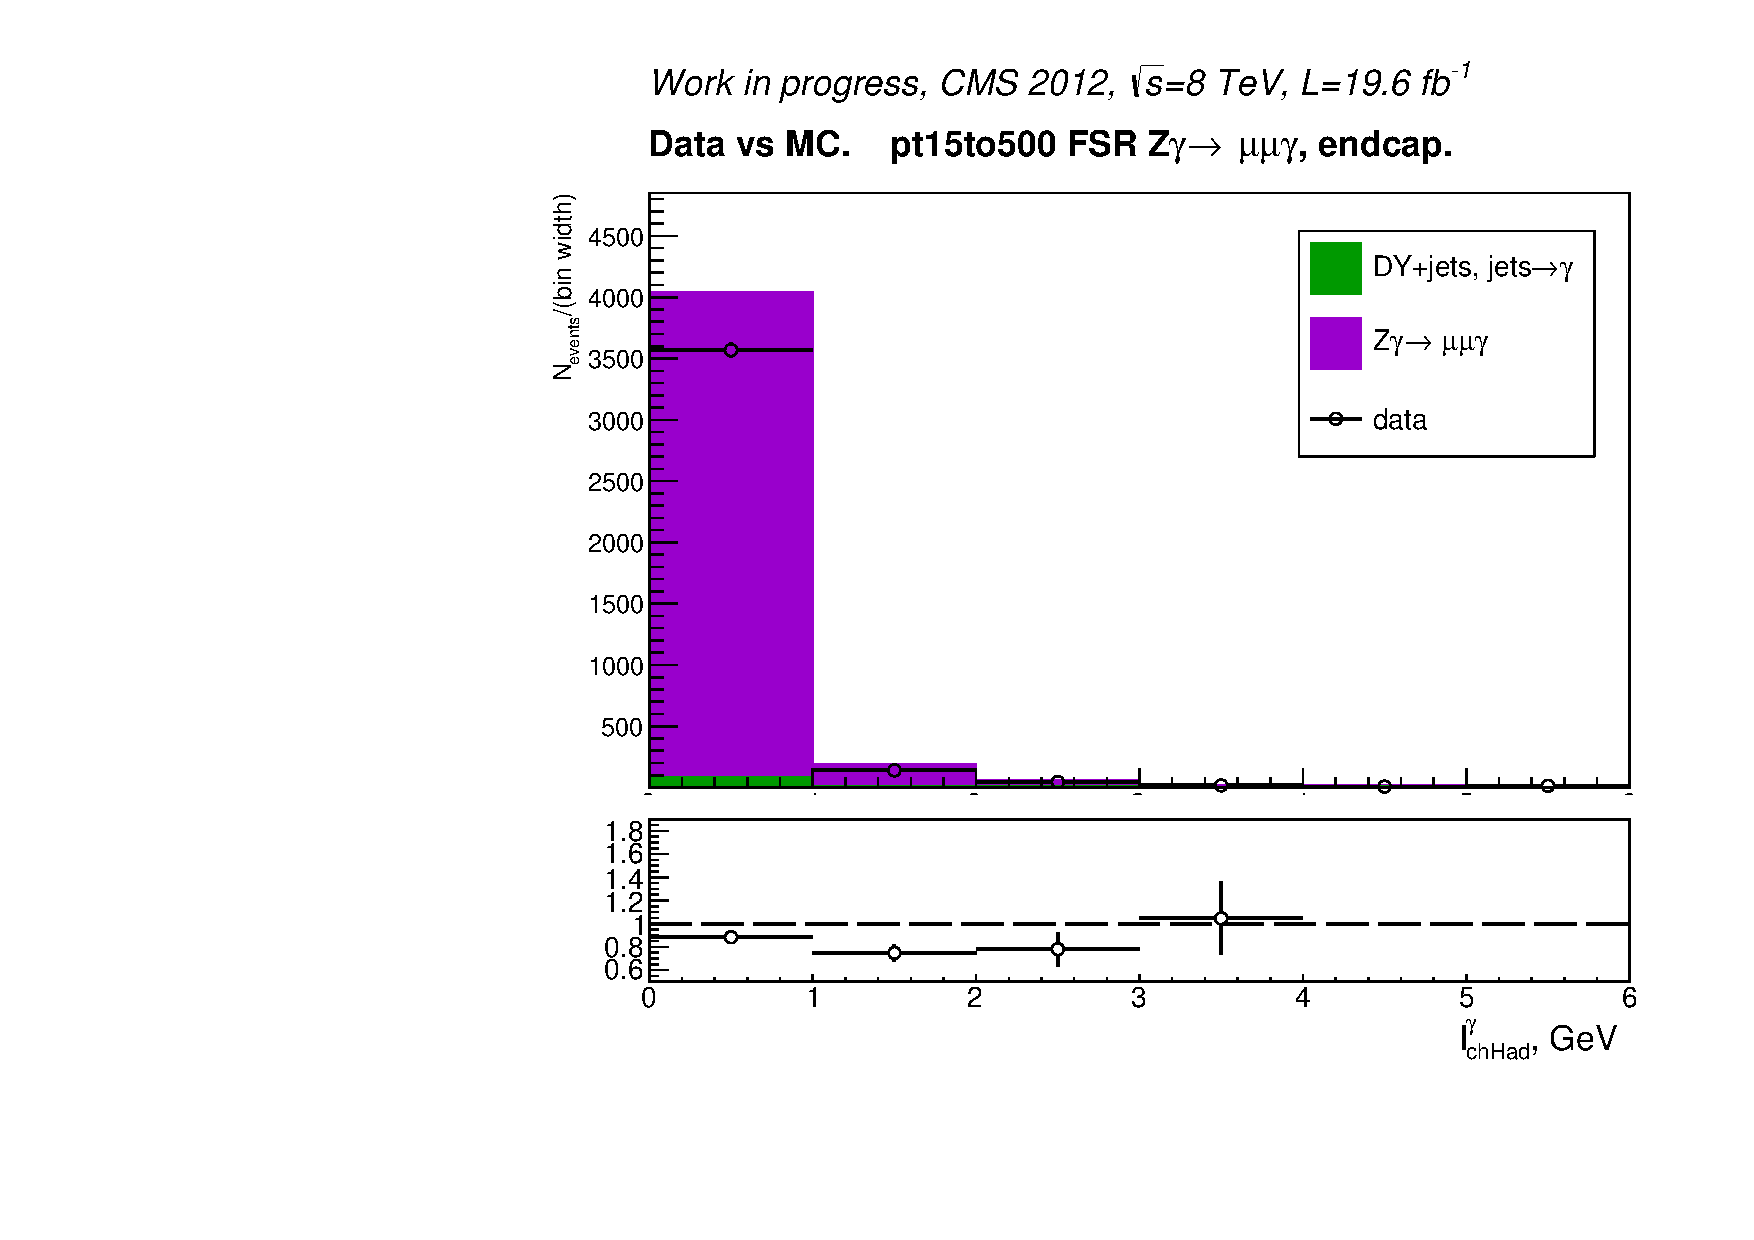
\includegraphics[width=0.45\textwidth]{../figs/figs_v11/MUON_ZGamma/PrepareYields/c_TotalDATAvsMC_Endcap__phoPFChIsoCorrFSR_pt15to500_FSR.pdf}\\
  \caption{$Z\gamma$-selected FSR events, data vs MC. $P_T^{\gamma}>10$~GeV. Distributions of $I_{chHad}^{\gamma}$ used for preparing real-$\gamma$ templates. Fake-$\gamma$ contribution to FSR region is subtracted based on DY+jets MC prediction to prepare real-$\gamma$ templates.}
  \label{fig:Zg_FSR_phoPFChIsoCorr}
  \end{center}
\end{figure}

\begin{figure}[htb]
  \begin{center}
   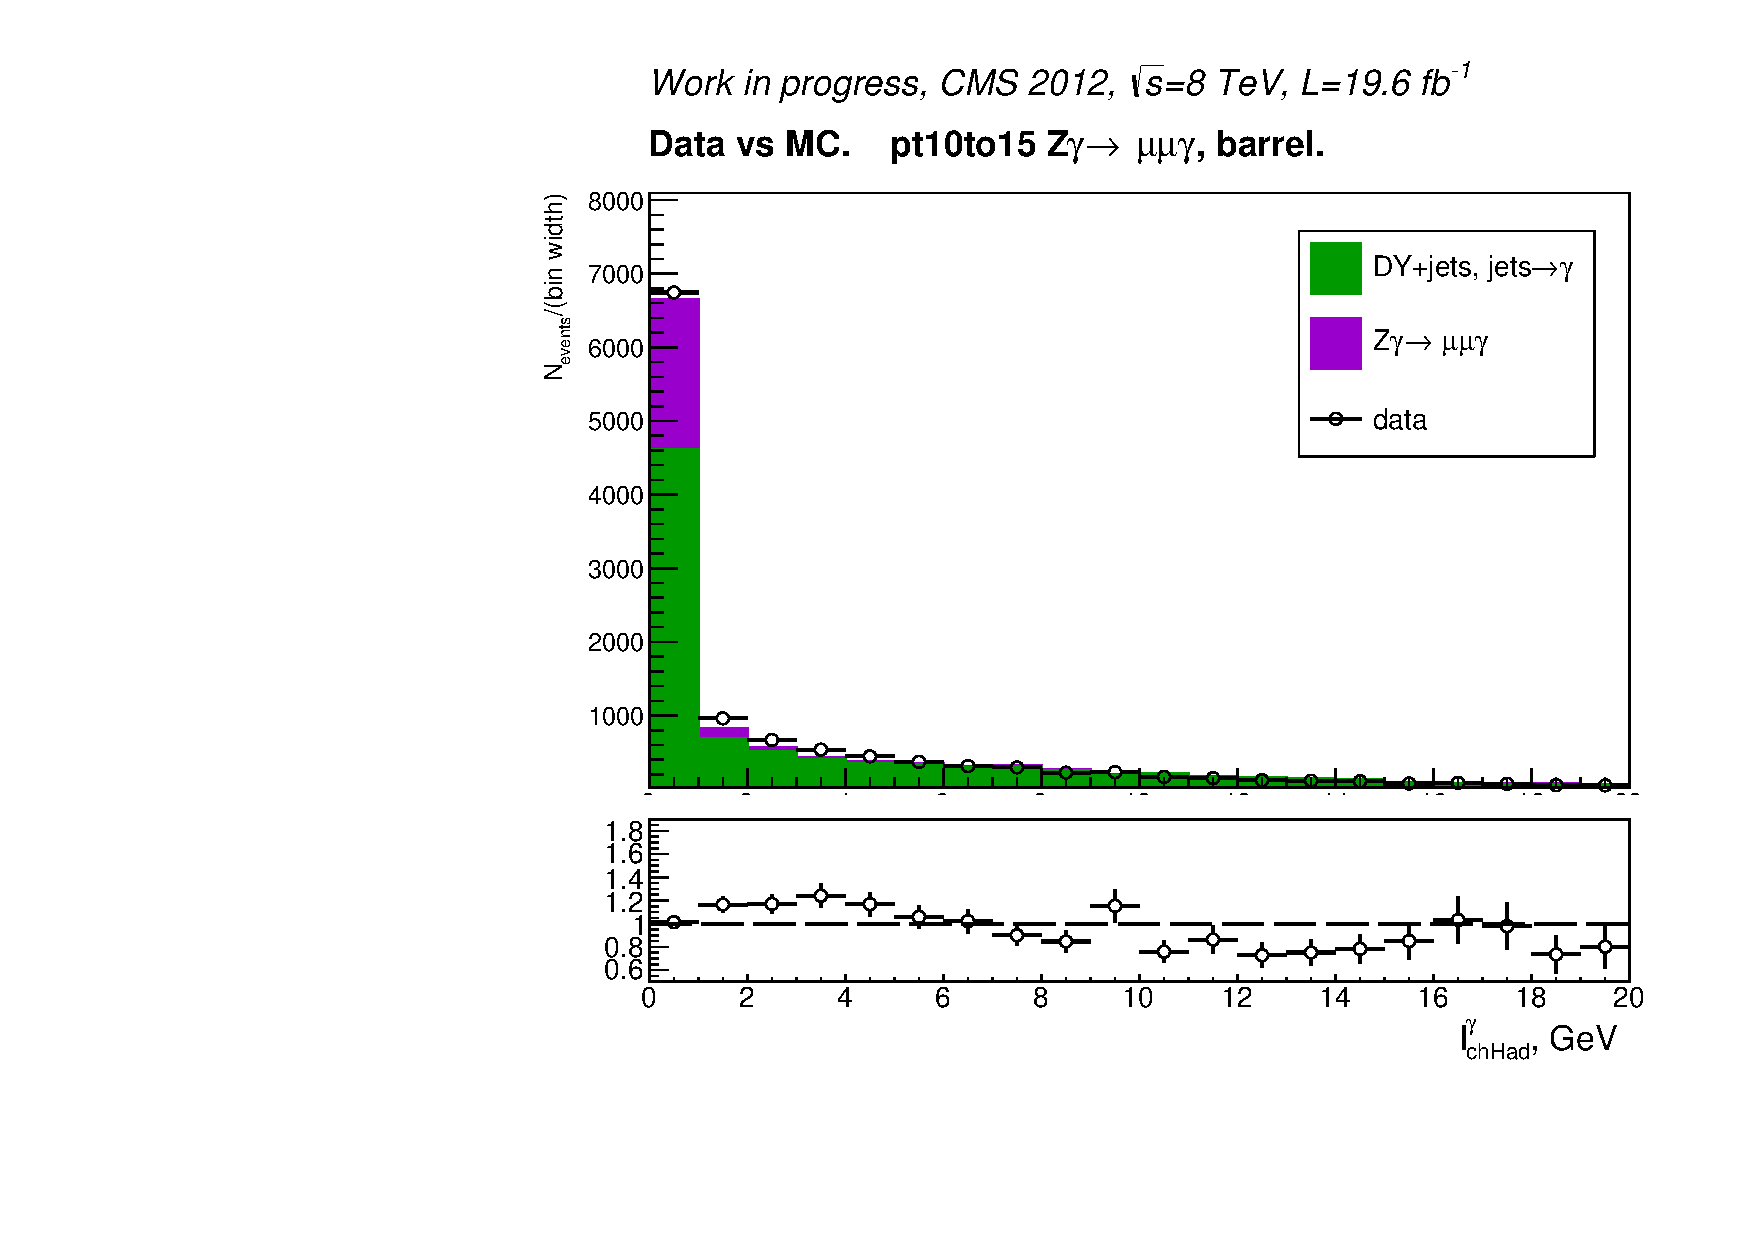
\includegraphics[width=0.45\textwidth]{../figs/figs_v11/MUON_ZGamma/PrepareYields/c_TotalDATAvsMC_Barrel__phoPFChIsoCorrFSR_EXCLUDED_pt10to15_.pdf}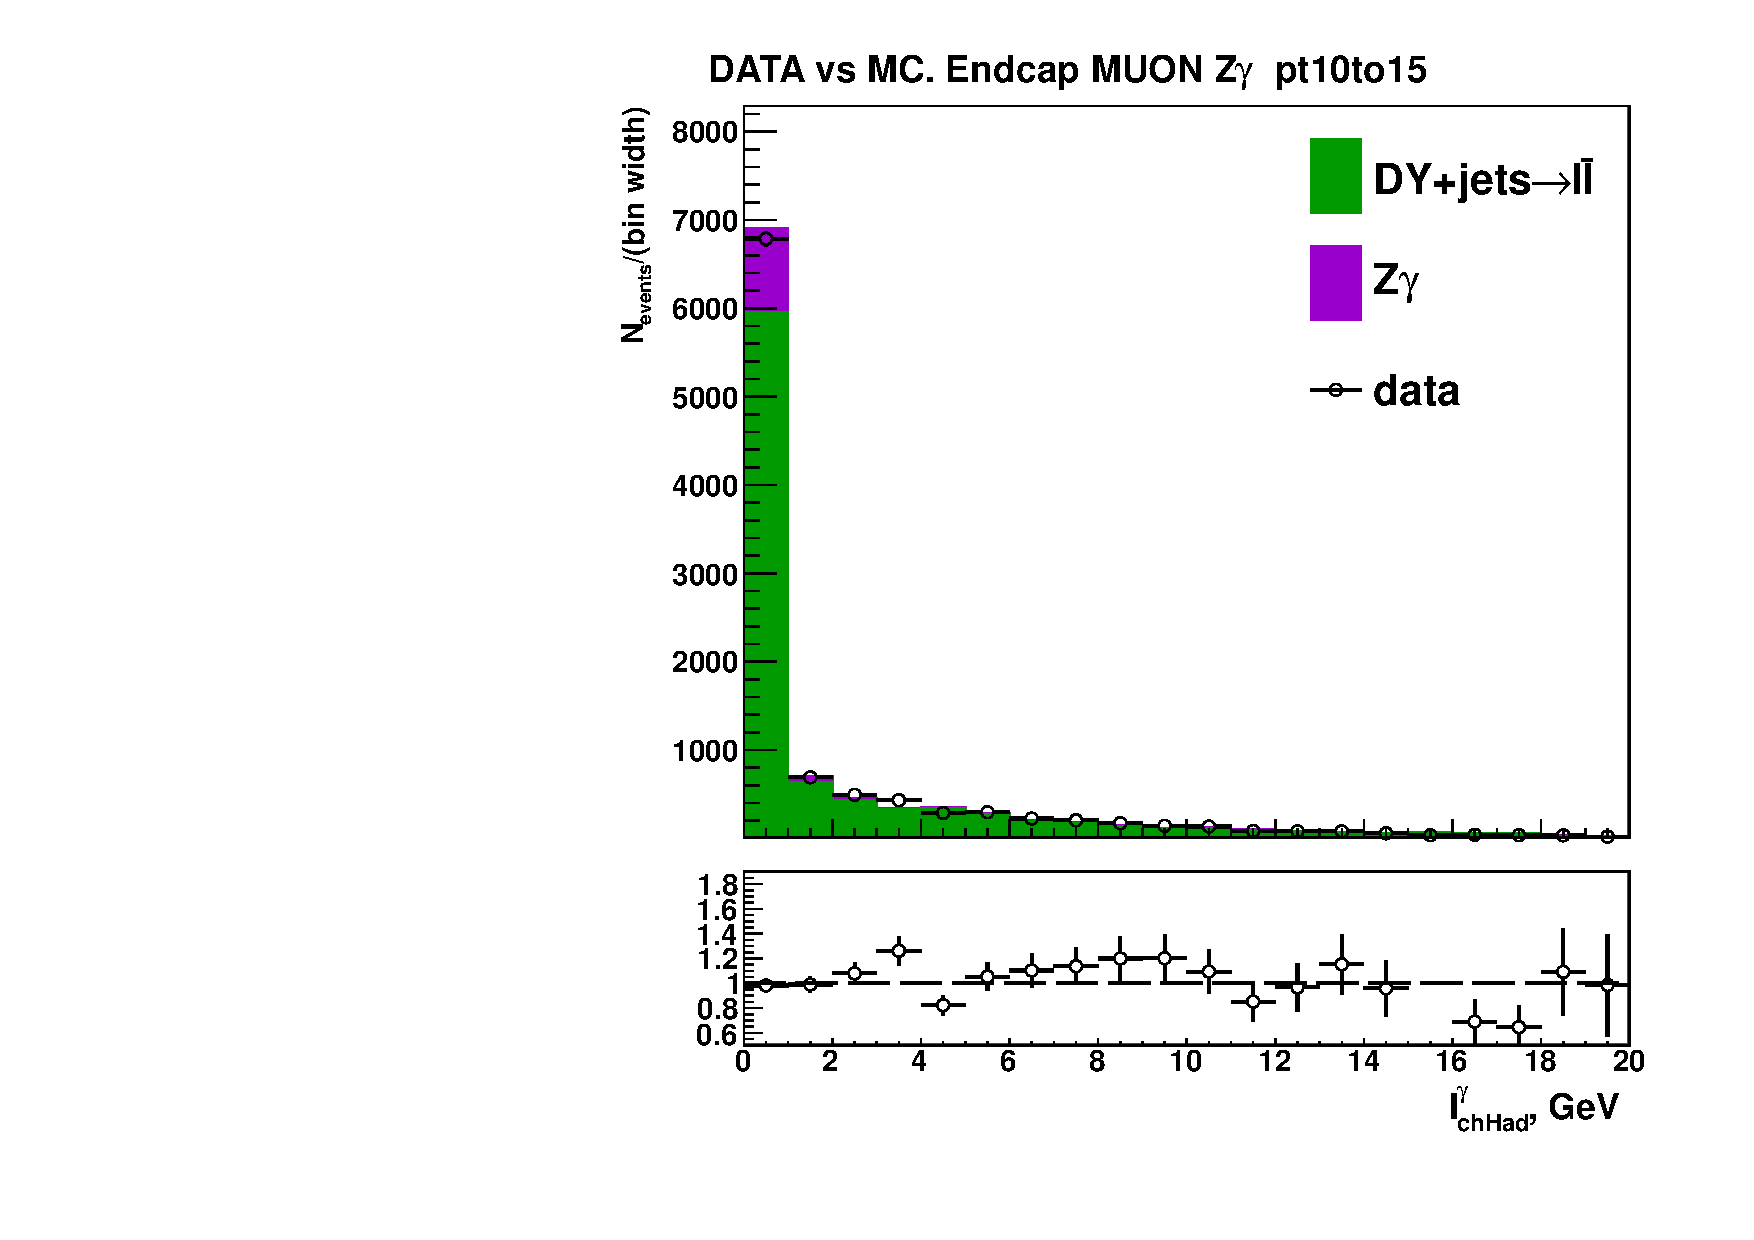
\includegraphics[width=0.45\textwidth]{../figs/figs_v11/MUON_ZGamma/PrepareYields/c_TotalDATAvsMC_Endcap__phoPFChIsoCorrFSR_EXCLUDED_pt10to15_.pdf}\\
  \caption{$Z\gamma$-selected ISR events, data vs MC. $10$~GeV$<P_T^{\gamma}<15$~GeV. Distributions of $I_{chHad}^{\gamma}$ used for preparing fake-$\gamma$ templates. Real-$\gamma$ contribution to ISR region is subtracted based on $Z\gamma$ signal MC prediction to prepare fake-$\gamma$ templates.}
  \label{fig:Zg_ISR_phoPFChIsoCorr_pt10to15}
  \end{center}
\end{figure}

\begin{figure}[htb]
  \begin{center}
   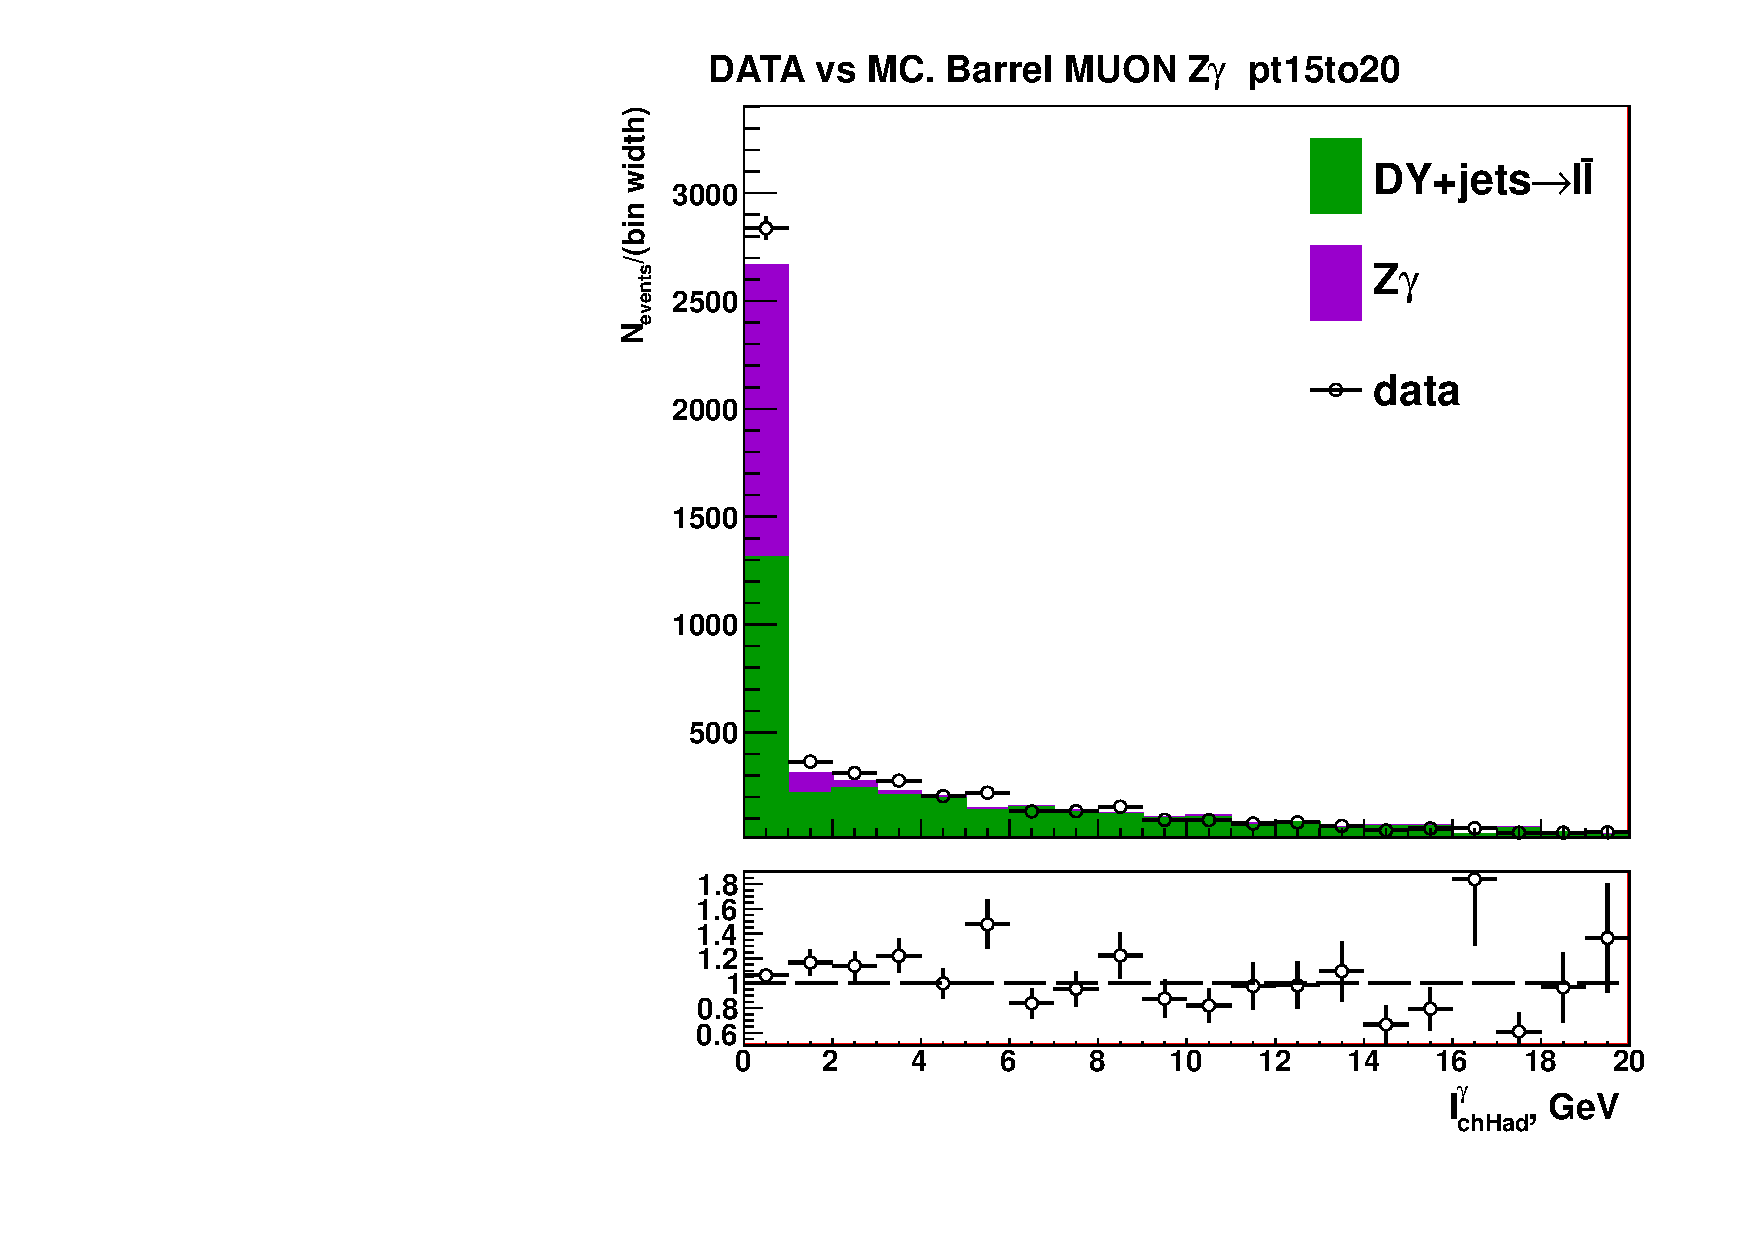
\includegraphics[width=0.32\textwidth]{../figs/figs_v11/MUON_ZGamma/PrepareYields/c_TotalDATAvsMC_Barrel__phoPFChIsoCorrFSR_EXCLUDED_pt15to20_.pdf}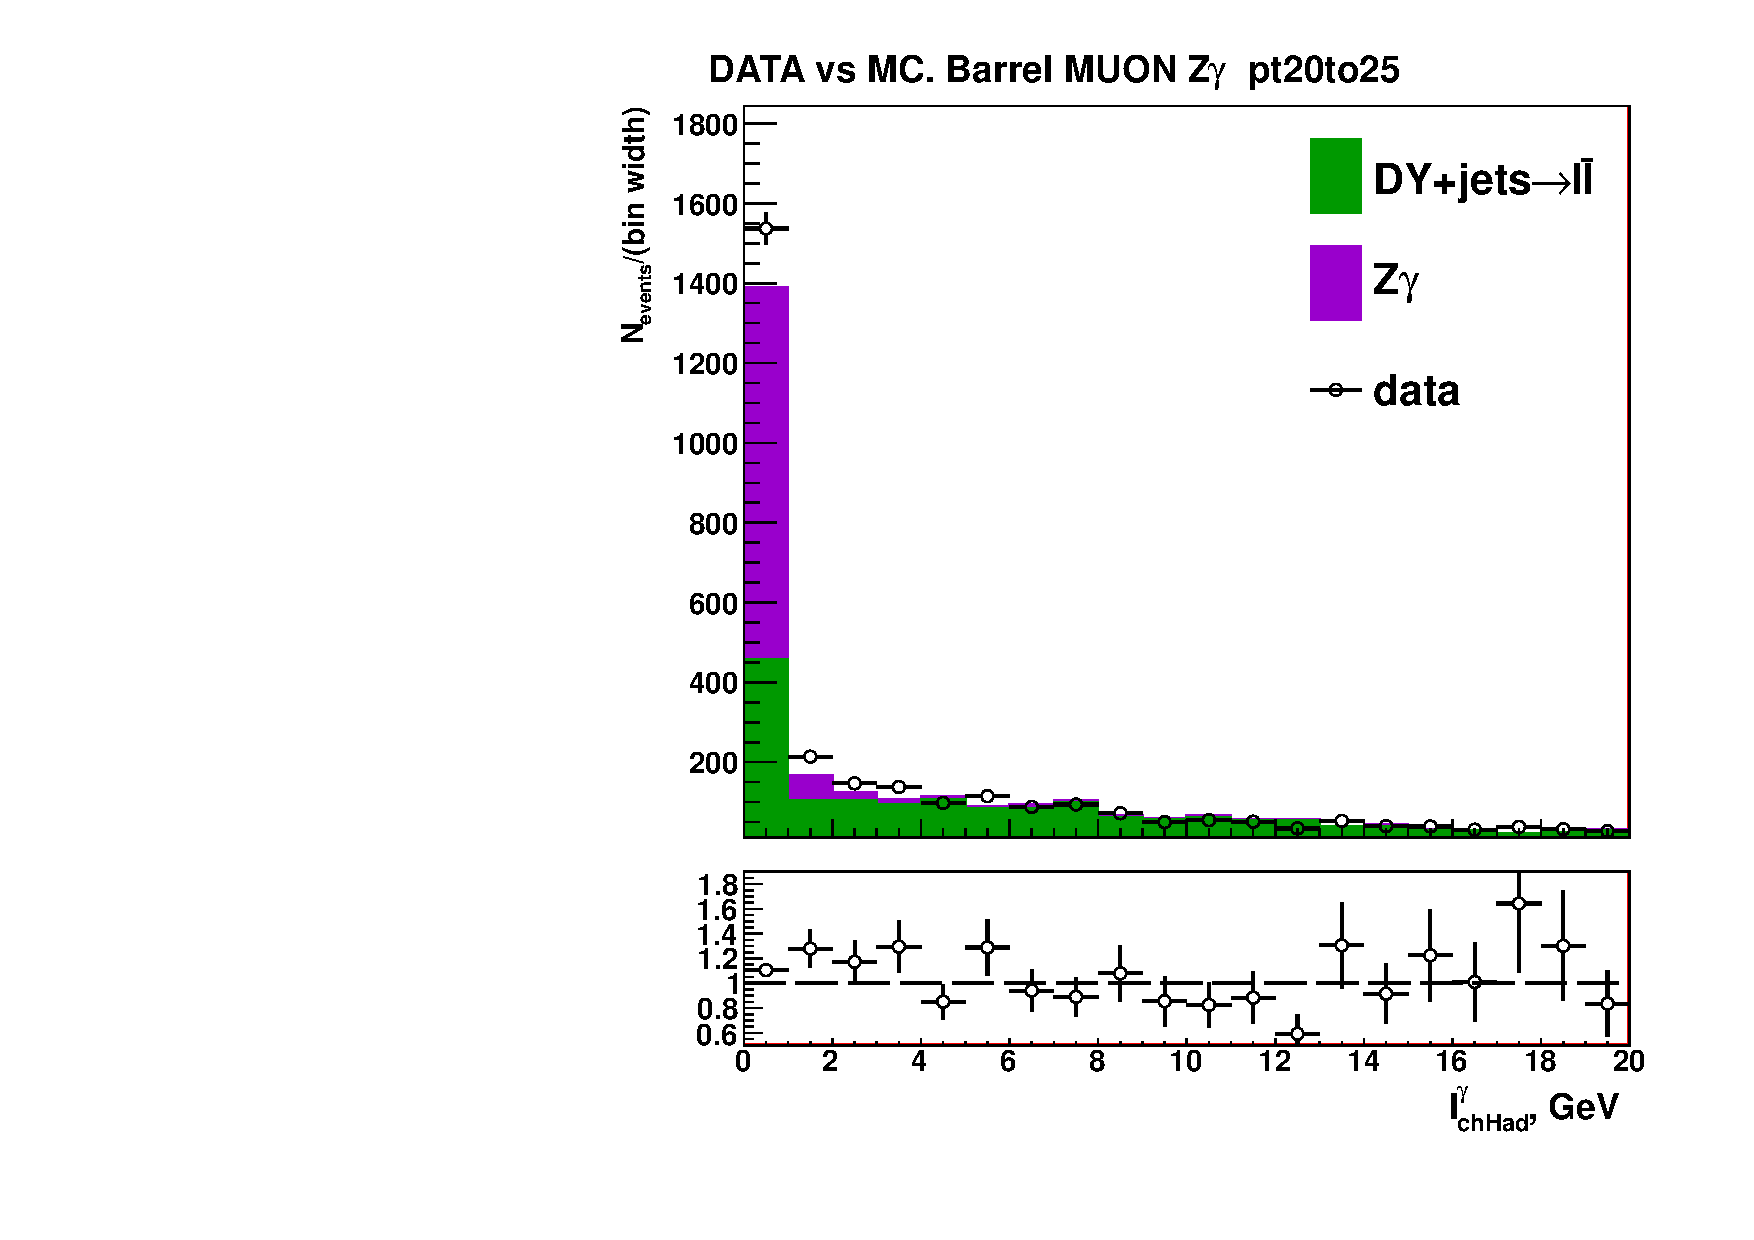
\includegraphics[width=0.32\textwidth]{../figs/figs_v11/MUON_ZGamma/PrepareYields/c_TotalDATAvsMC_Barrel__phoPFChIsoCorrFSR_EXCLUDED_pt20to25_.pdf}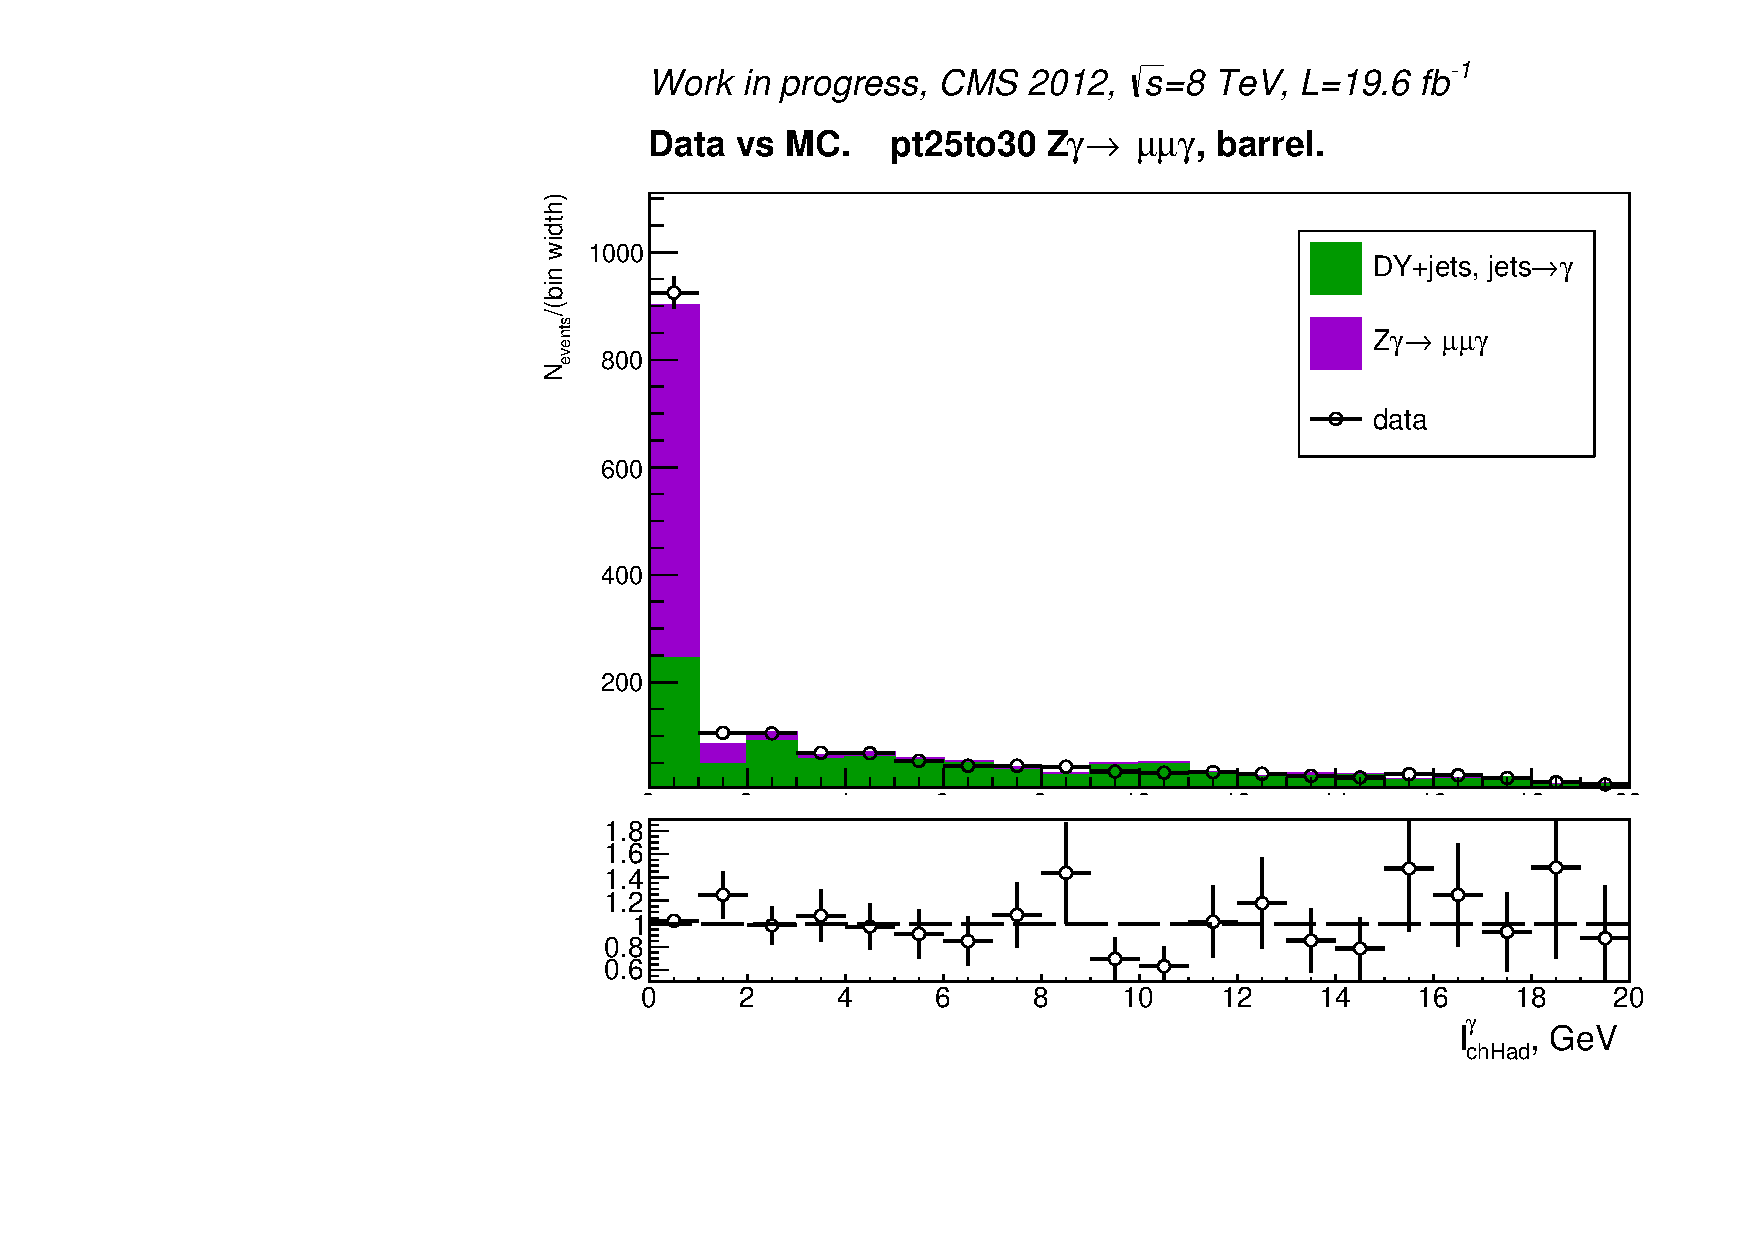
\includegraphics[width=0.32\textwidth]{../figs/figs_v11/MUON_ZGamma/PrepareYields/c_TotalDATAvsMC_Barrel__phoPFChIsoCorrFSR_EXCLUDED_pt25to30_.pdf}\\
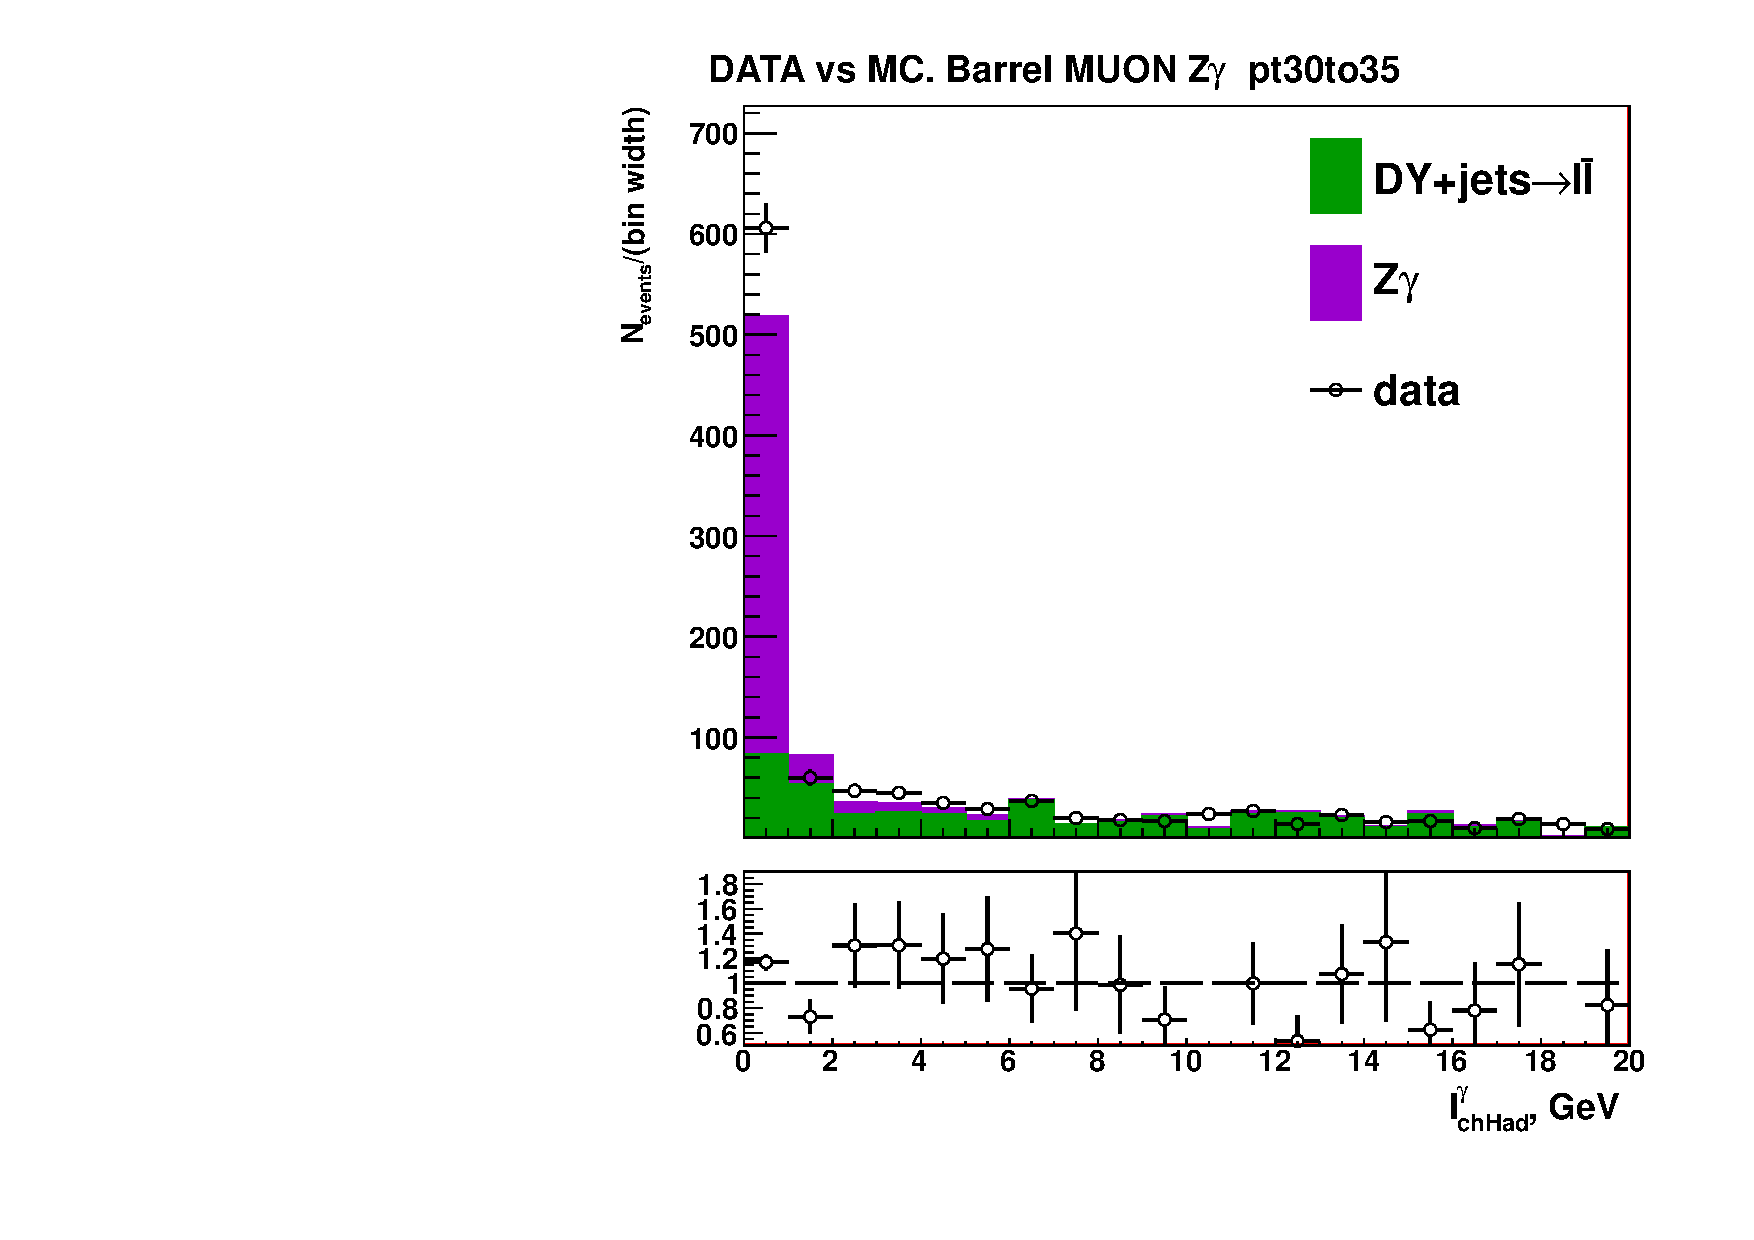
\includegraphics[width=0.32\textwidth]{../figs/figs_v11/MUON_ZGamma/PrepareYields/c_TotalDATAvsMC_Barrel__phoPFChIsoCorrFSR_EXCLUDED_pt30to35_.pdf}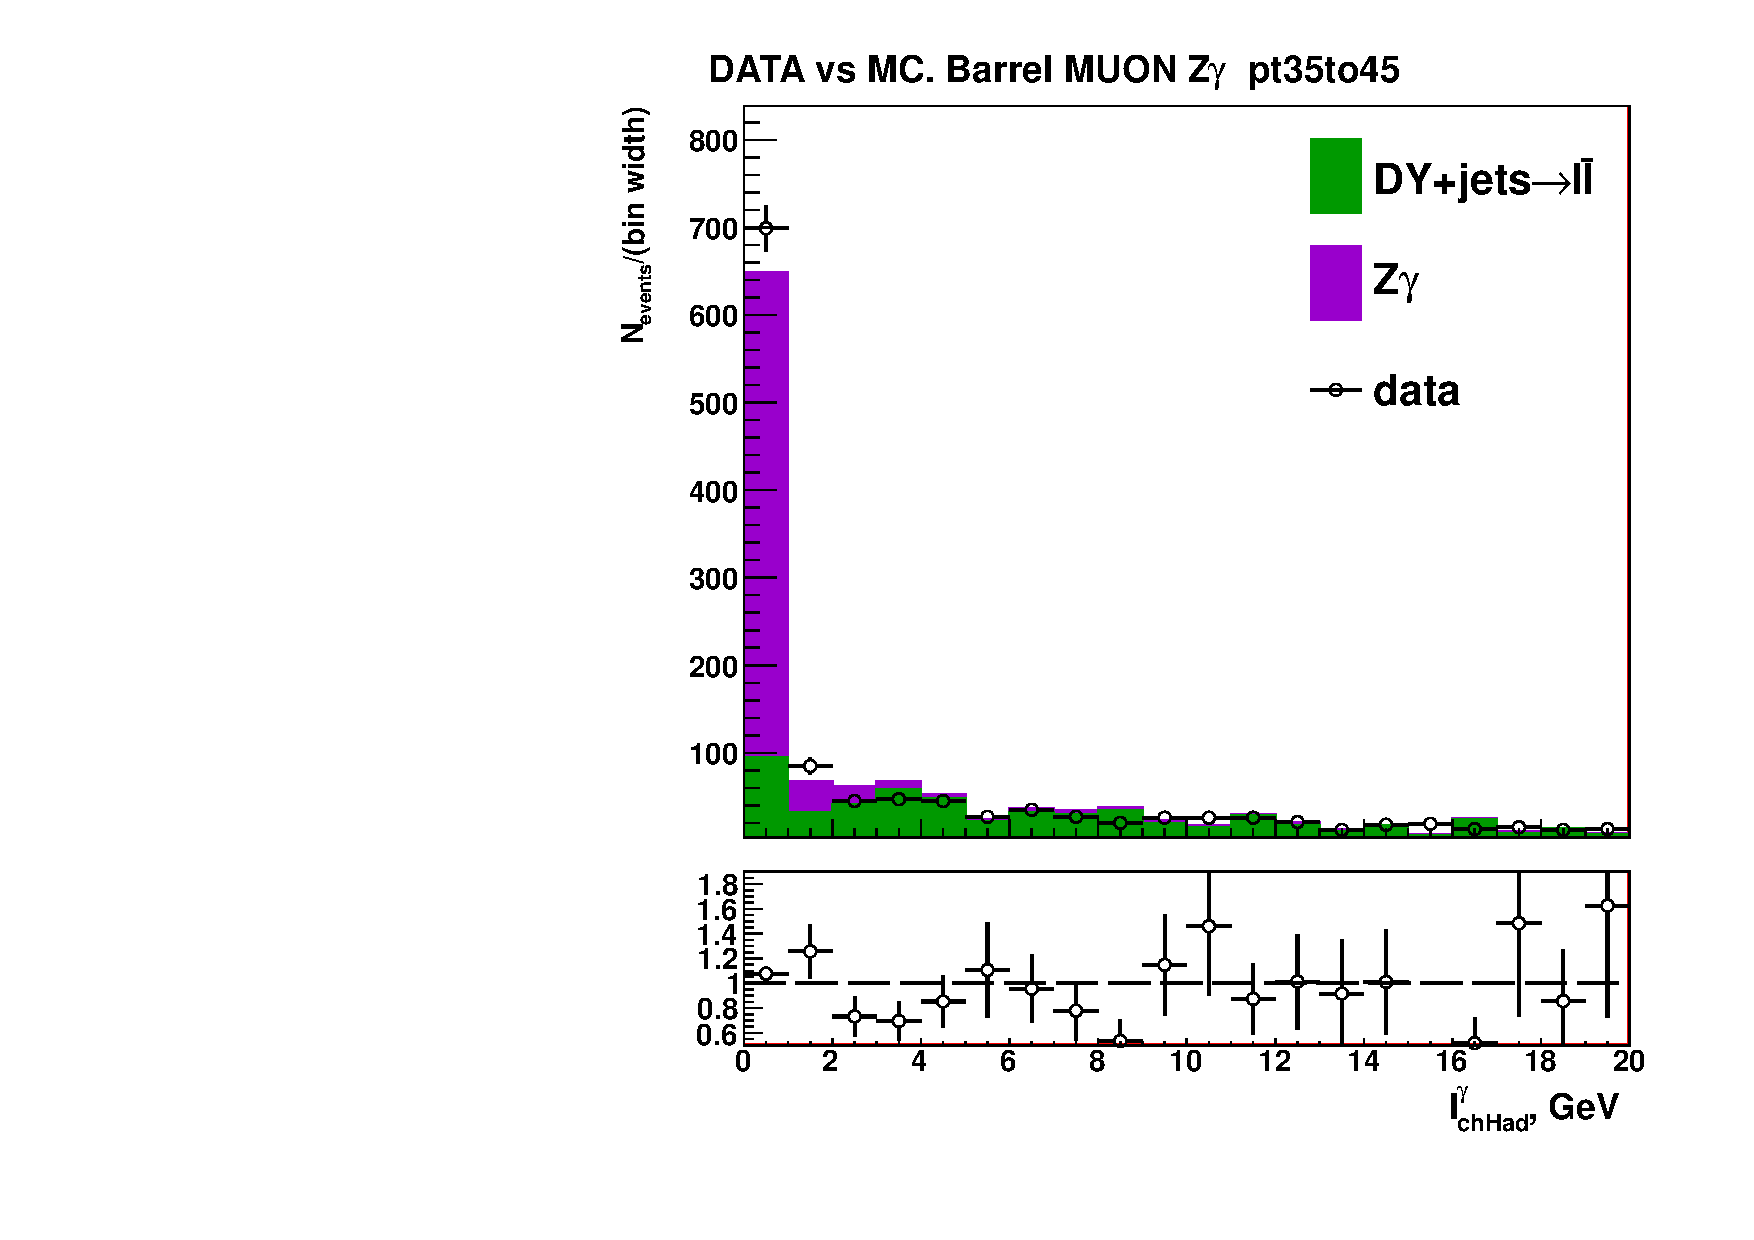
\includegraphics[width=0.32\textwidth]{../figs/figs_v11/MUON_ZGamma/PrepareYields/c_TotalDATAvsMC_Barrel__phoPFChIsoCorrFSR_EXCLUDED_pt35to45_.pdf}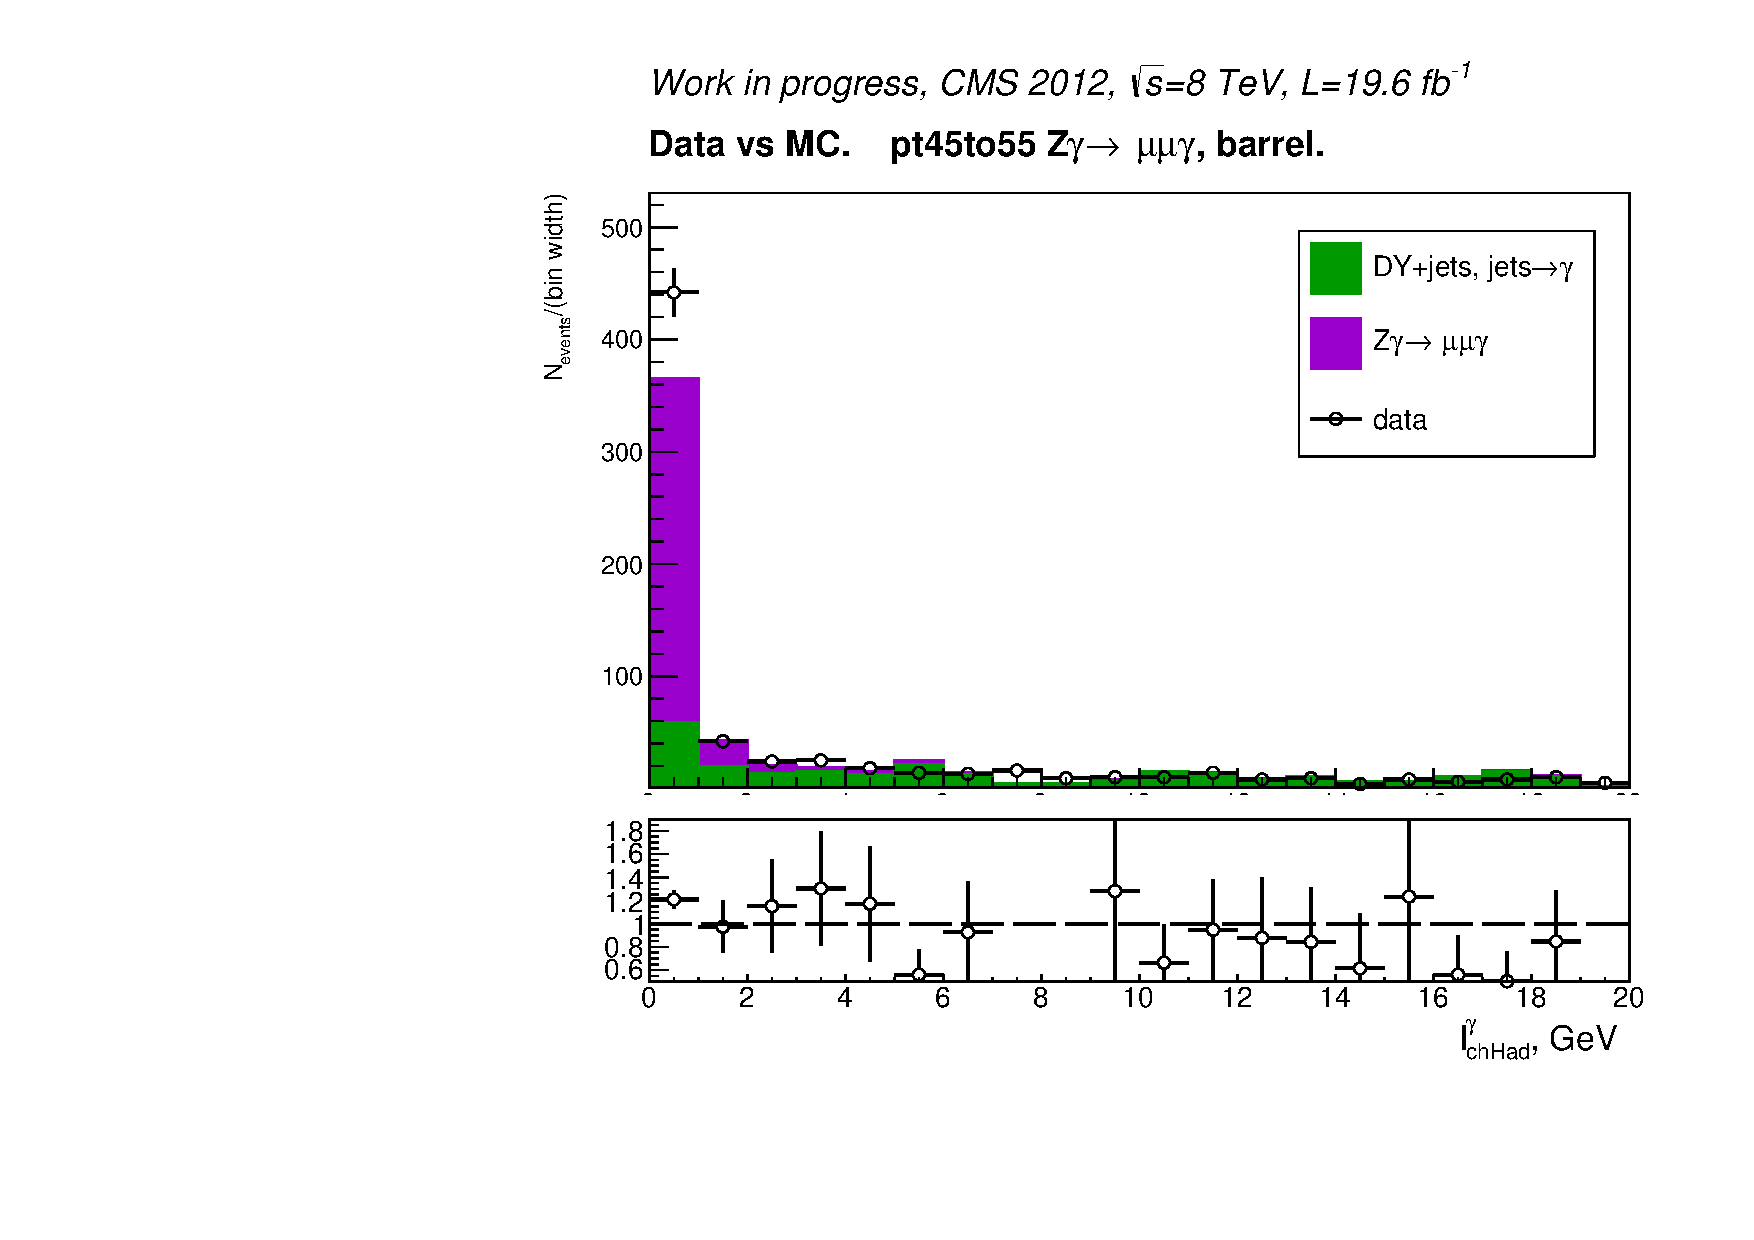
\includegraphics[width=0.32\textwidth]{../figs/figs_v11/MUON_ZGamma/PrepareYields/c_TotalDATAvsMC_Barrel__phoPFChIsoCorrFSR_EXCLUDED_pt45to55_.pdf}\\
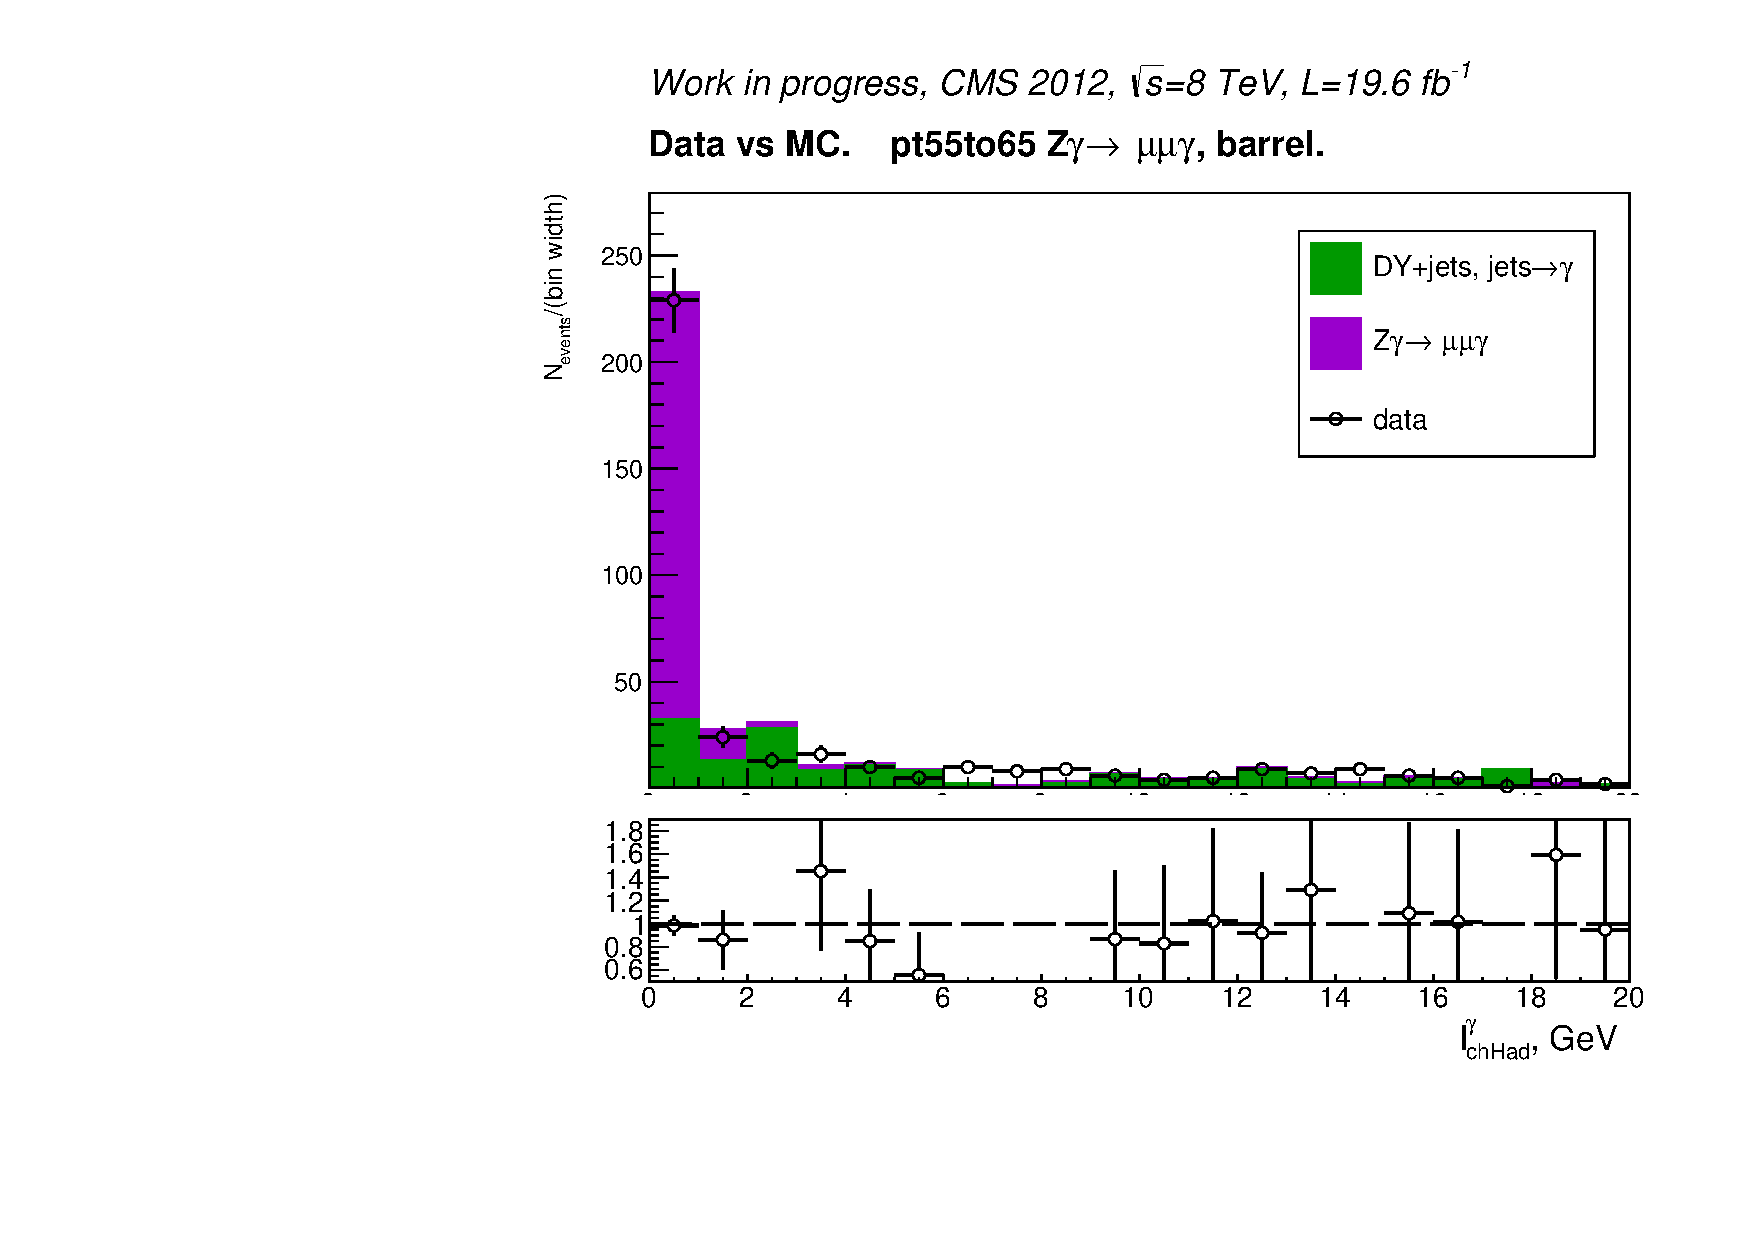
\includegraphics[width=0.32\textwidth]{../figs/figs_v11/MUON_ZGamma/PrepareYields/c_TotalDATAvsMC_Barrel__phoPFChIsoCorrFSR_EXCLUDED_pt55to65_.pdf}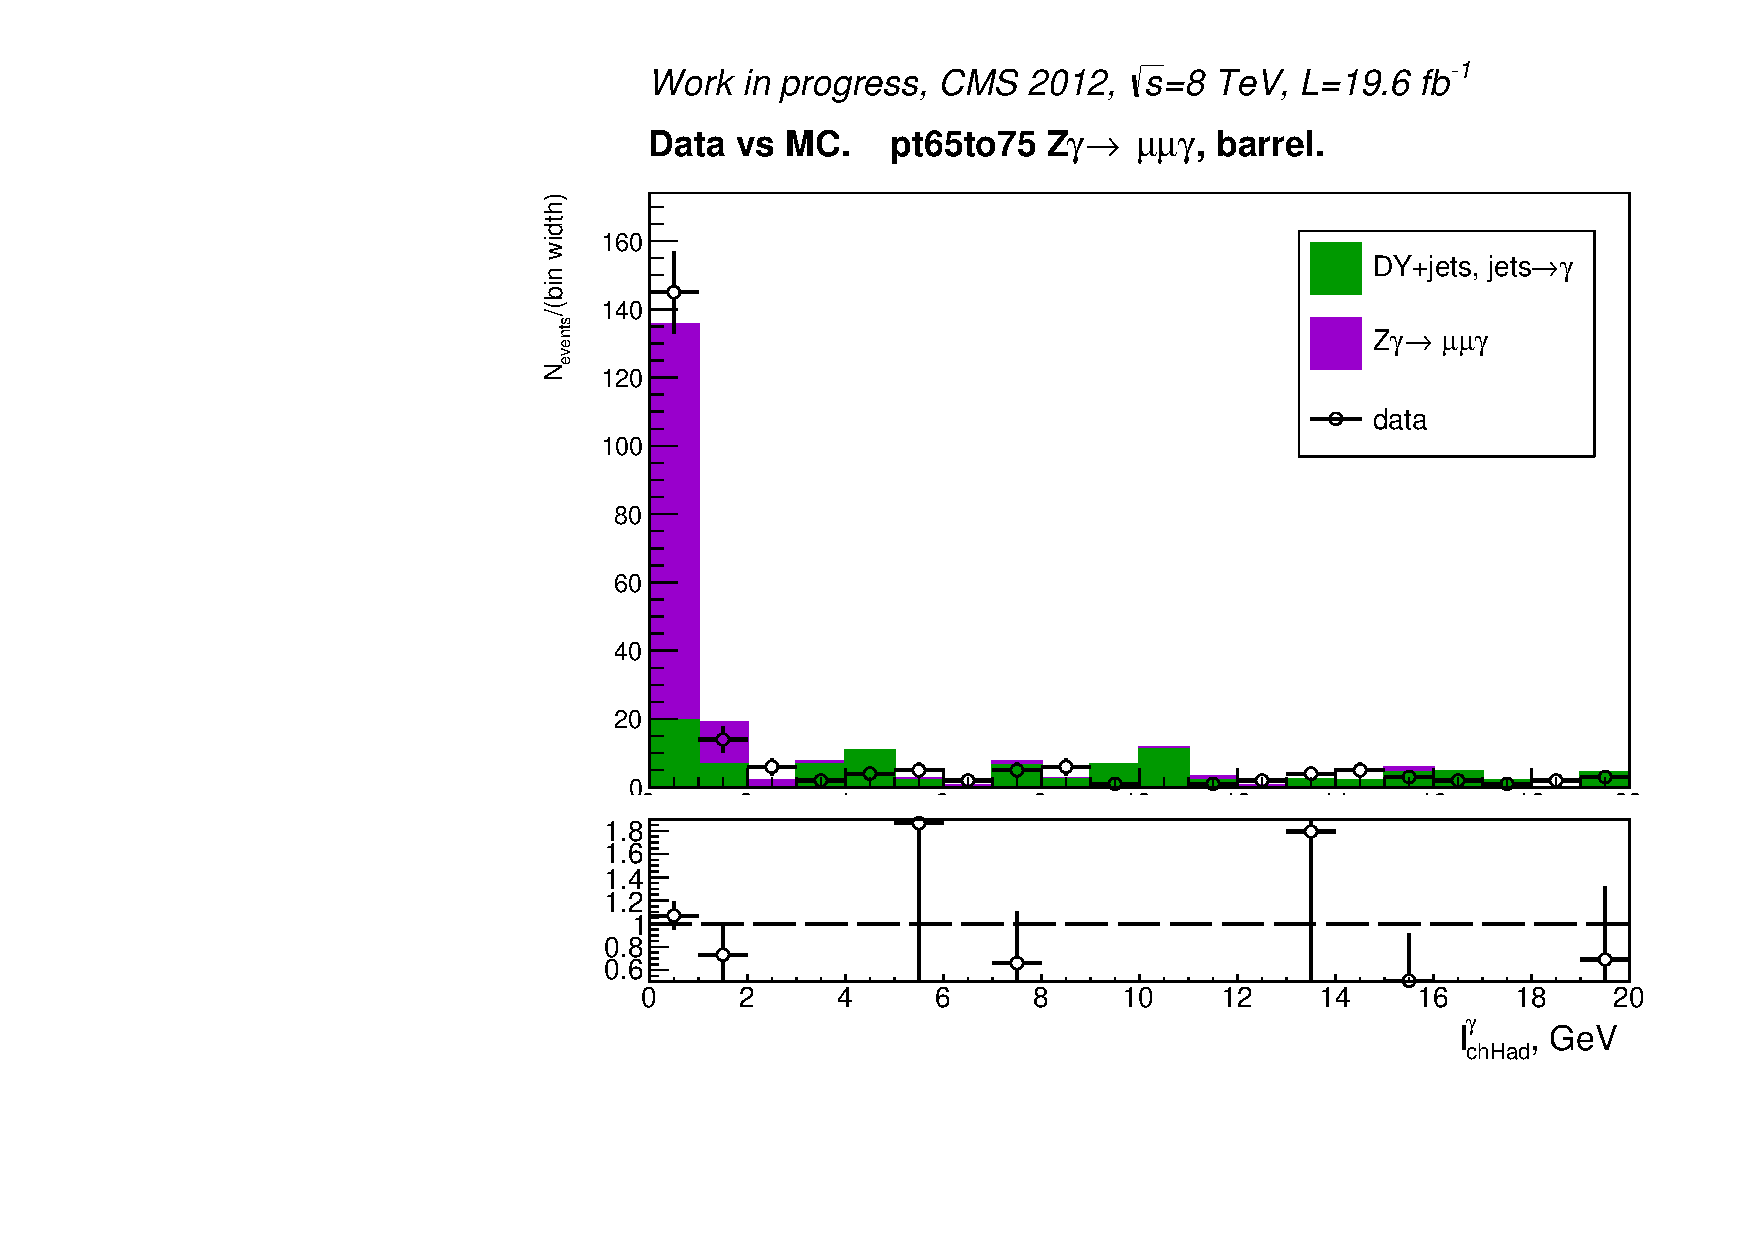
\includegraphics[width=0.32\textwidth]{../figs/figs_v11/MUON_ZGamma/PrepareYields/c_TotalDATAvsMC_Barrel__phoPFChIsoCorrFSR_EXCLUDED_pt65to75_.pdf}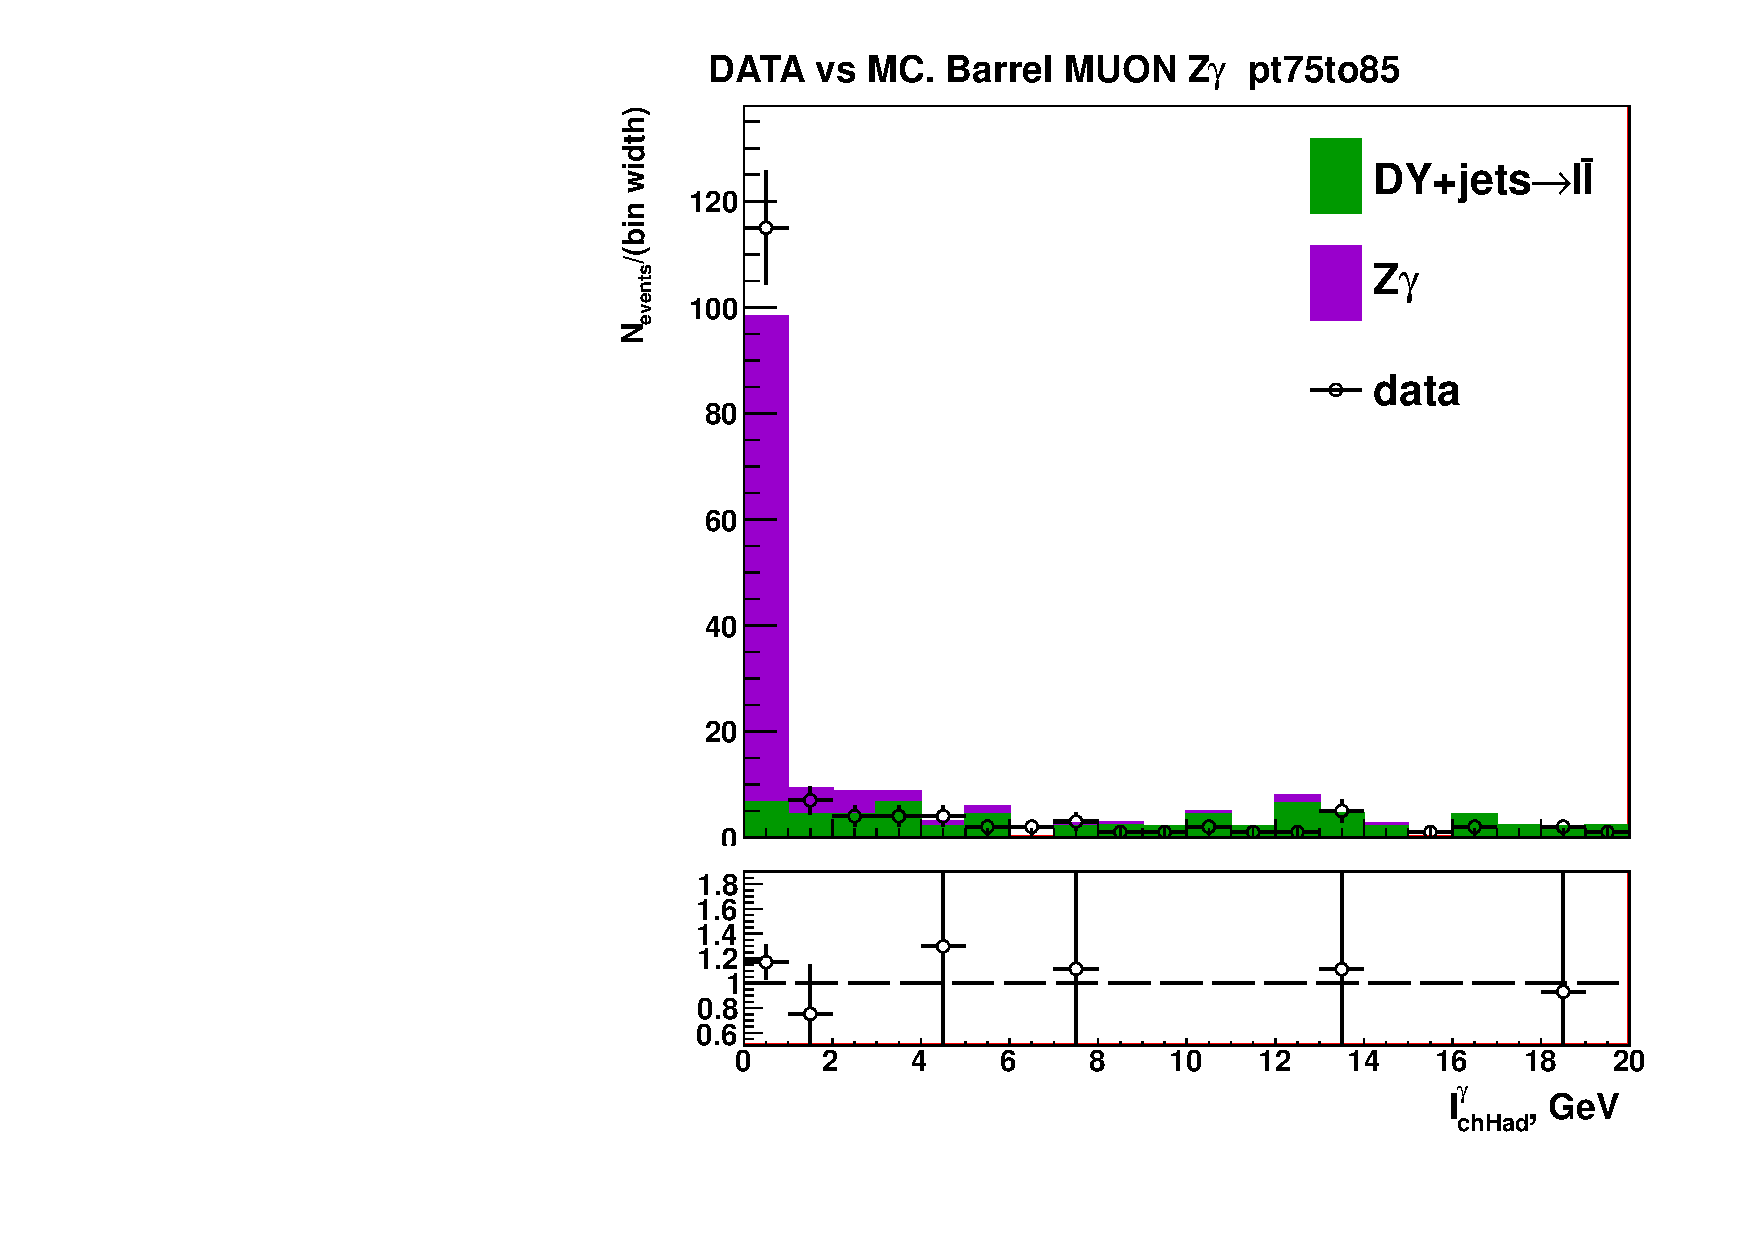
\includegraphics[width=0.32\textwidth]{../figs/figs_v11/MUON_ZGamma/PrepareYields/c_TotalDATAvsMC_Barrel__phoPFChIsoCorrFSR_EXCLUDED_pt75to85_.pdf}\\
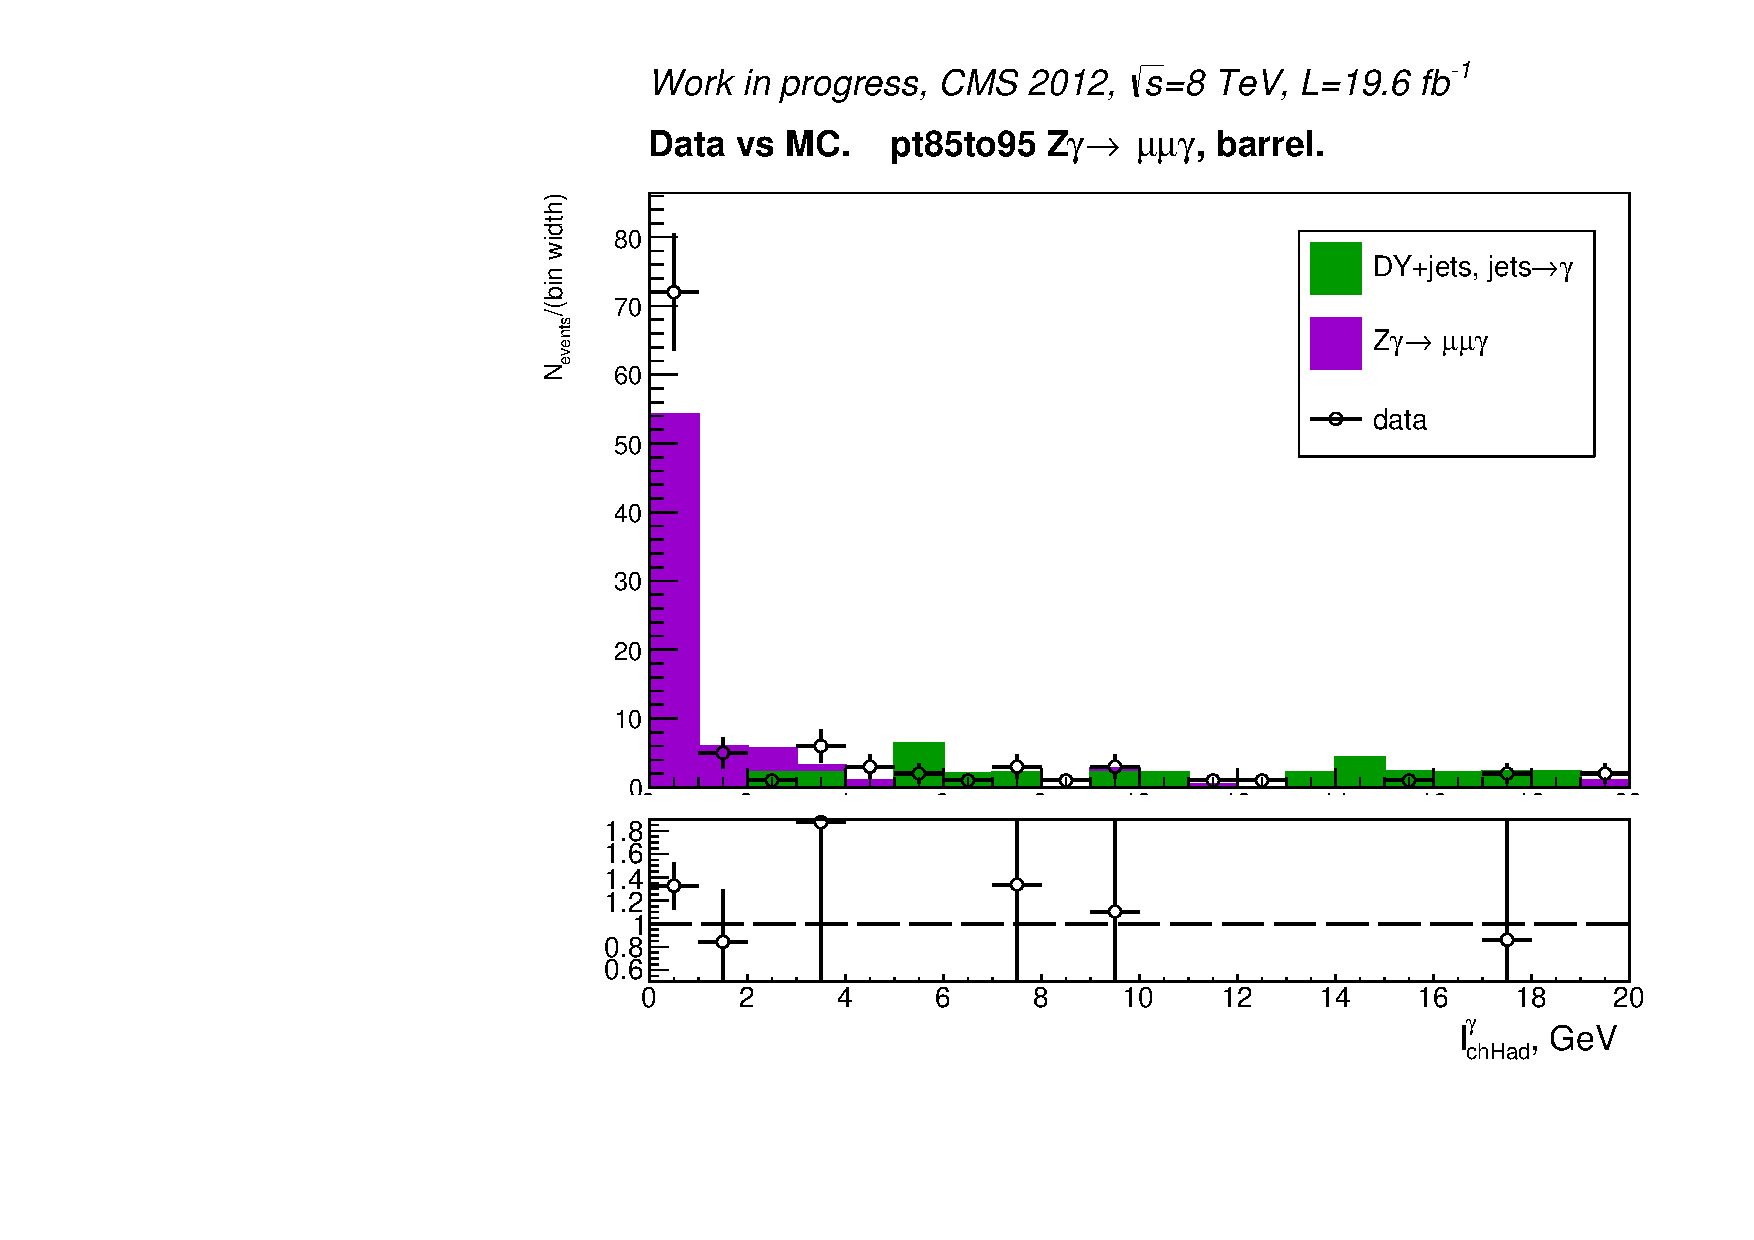
\includegraphics[width=0.32\textwidth]{../figs/figs_v11/MUON_ZGamma/PrepareYields/c_TotalDATAvsMC_Barrel__phoPFChIsoCorrFSR_EXCLUDED_pt85to95_.pdf}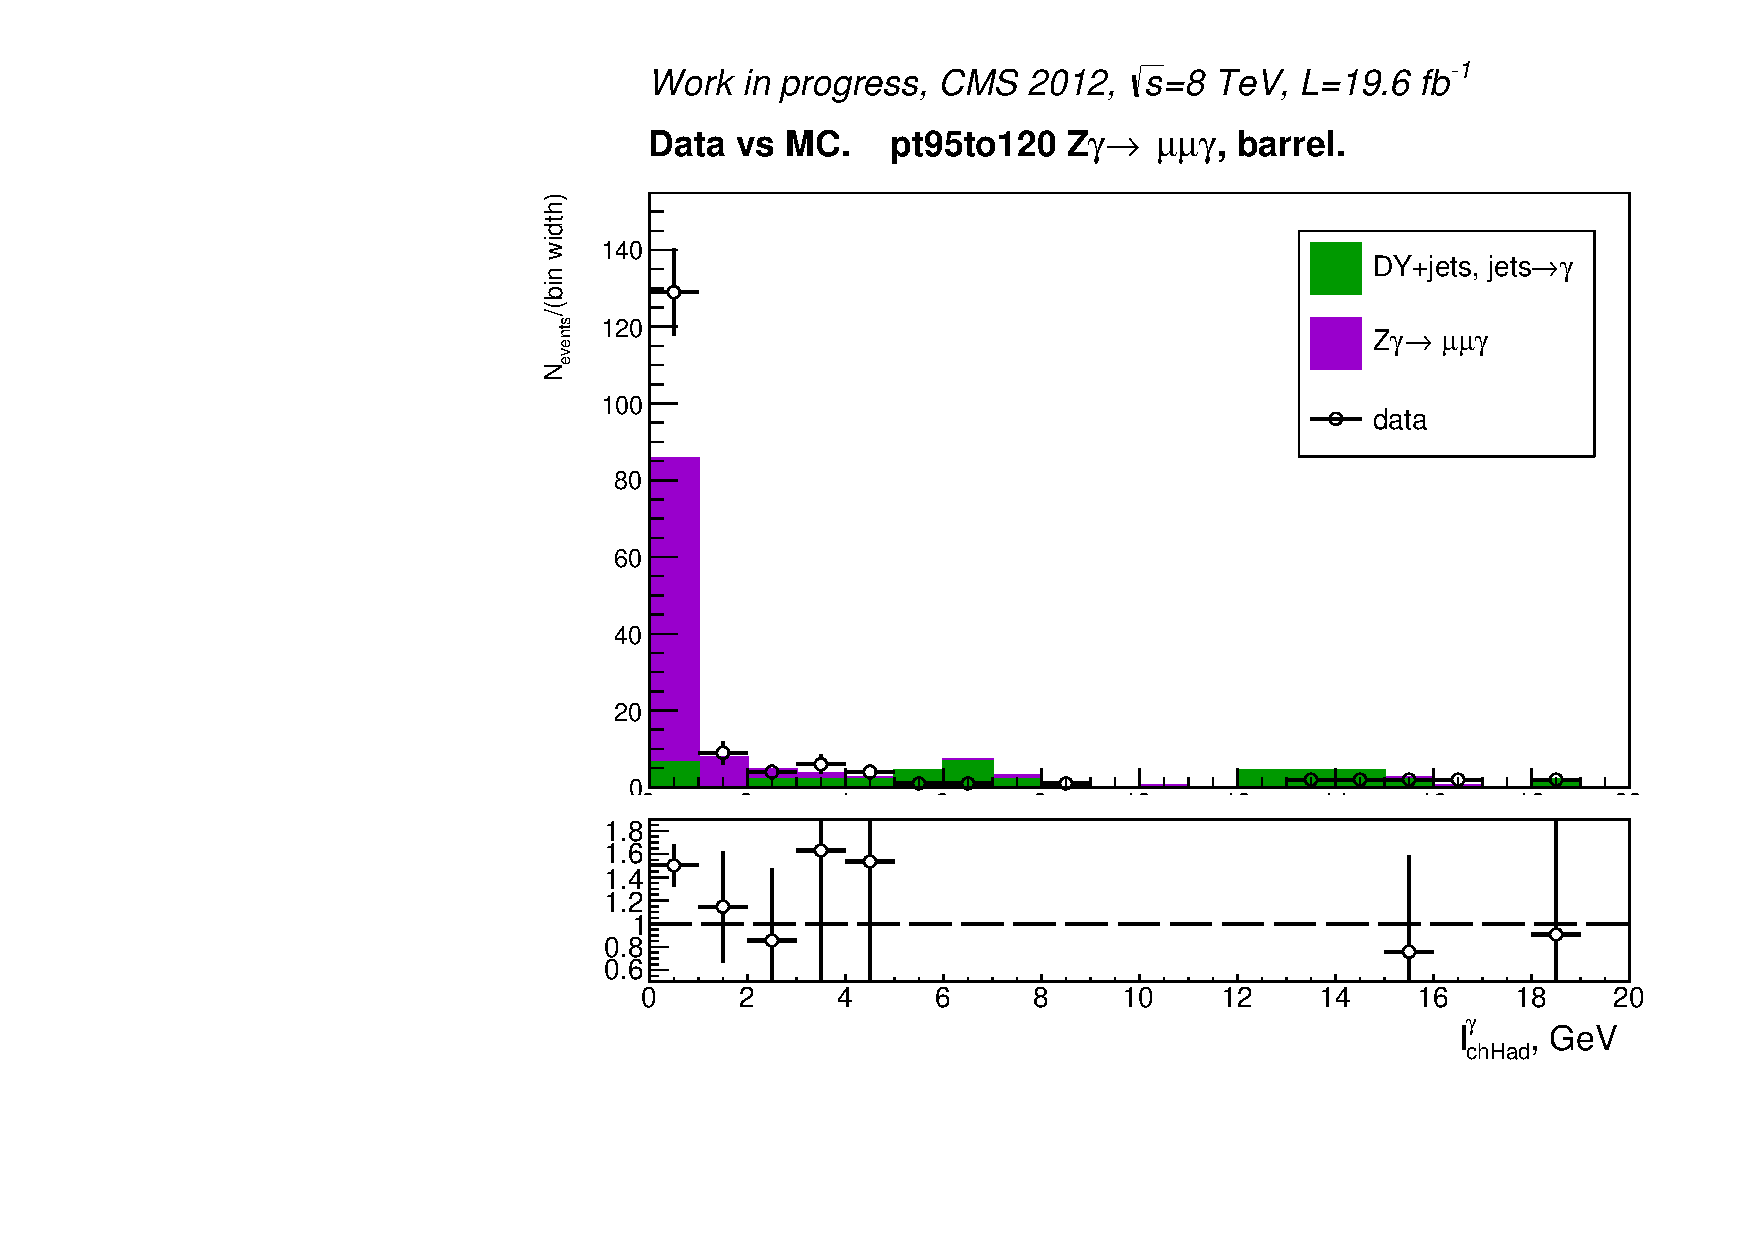
\includegraphics[width=0.32\textwidth]{../figs/figs_v11/MUON_ZGamma/PrepareYields/c_TotalDATAvsMC_Barrel__phoPFChIsoCorrFSR_EXCLUDED_pt95to120_.pdf}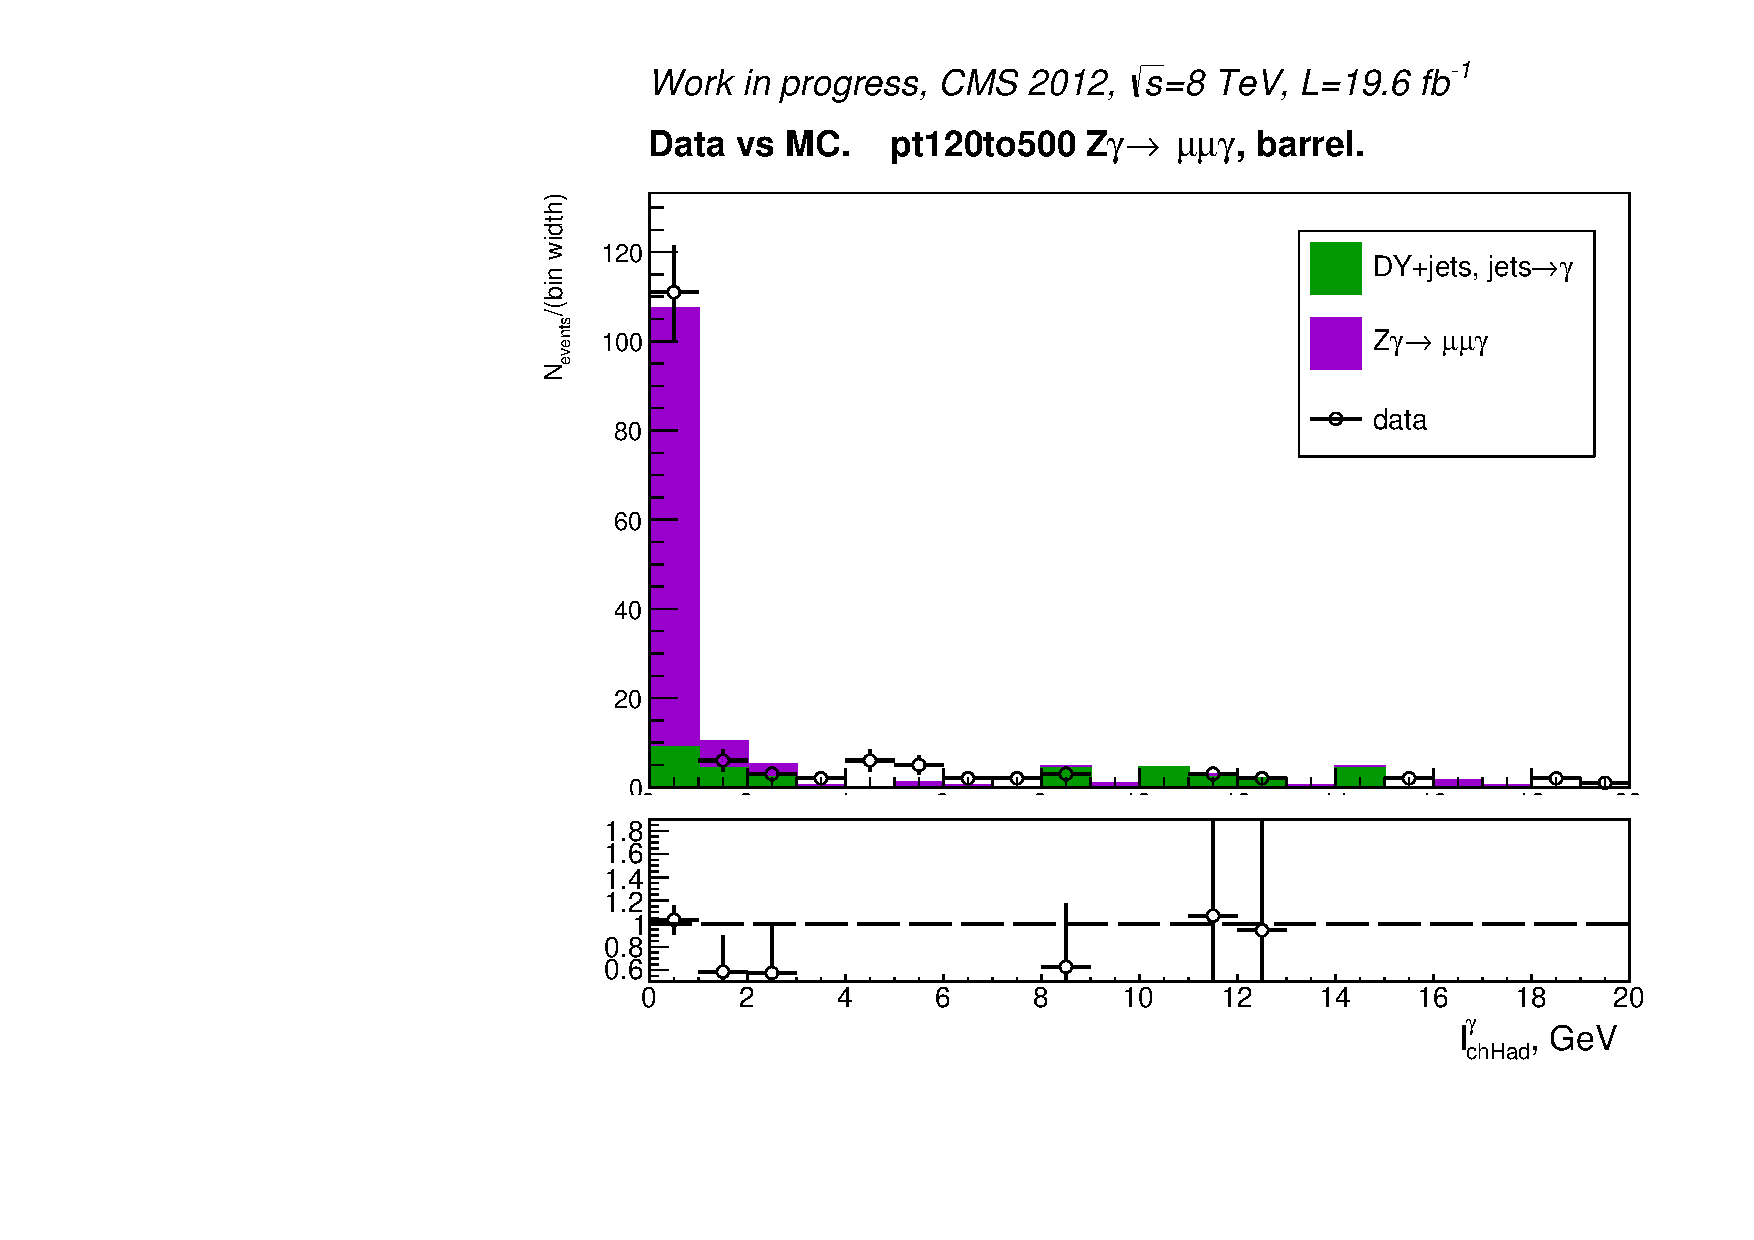
\includegraphics[width=0.32\textwidth]{../figs/figs_v11/MUON_ZGamma/PrepareYields/c_TotalDATAvsMC_Barrel__phoPFChIsoCorrFSR_EXCLUDED_pt120to500_.pdf}\\
  \caption{$Z\gamma$-selected ISR events, data vs MC. $15$~GeV$<P_T^{\gamma}<500$~GeV, Barrel photons. Distributions of $I_{chHad}^{\gamma}$ used for preparing fake-$\gamma$ templates. Real-$\gamma$ contribution to ISR region is subtracted based on $Z\gamma$ signal MC prediction to prepare fake-$\gamma$ templates.}
  \label{fig:Zg_ISR_phoPFChIsoCorr_Barrel}
  \end{center}
\end{figure}

\begin{figure}[htb]
  \begin{center}
   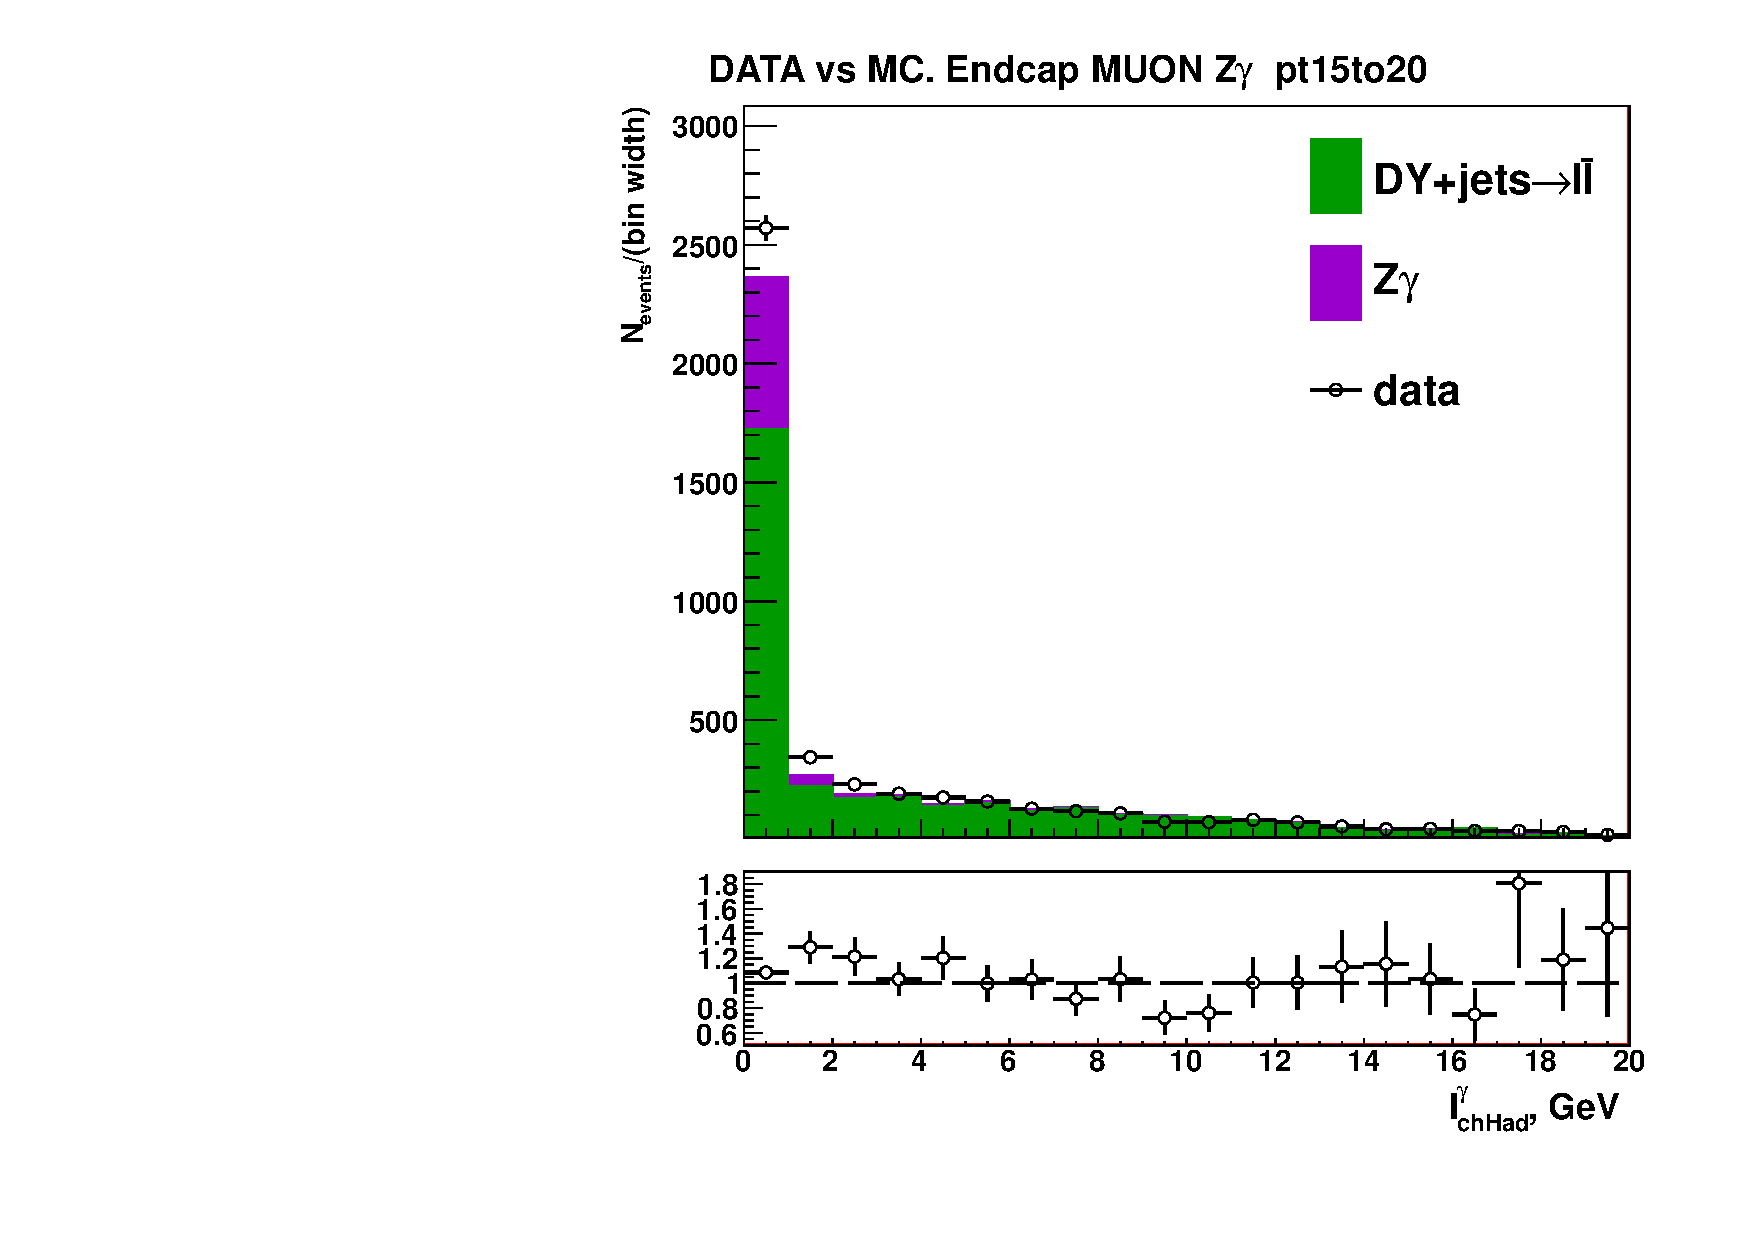
\includegraphics[width=0.32\textwidth]{../figs/figs_v11/MUON_ZGamma/PrepareYields/c_TotalDATAvsMC_Endcap__phoPFChIsoCorrFSR_EXCLUDED_pt15to20_.pdf}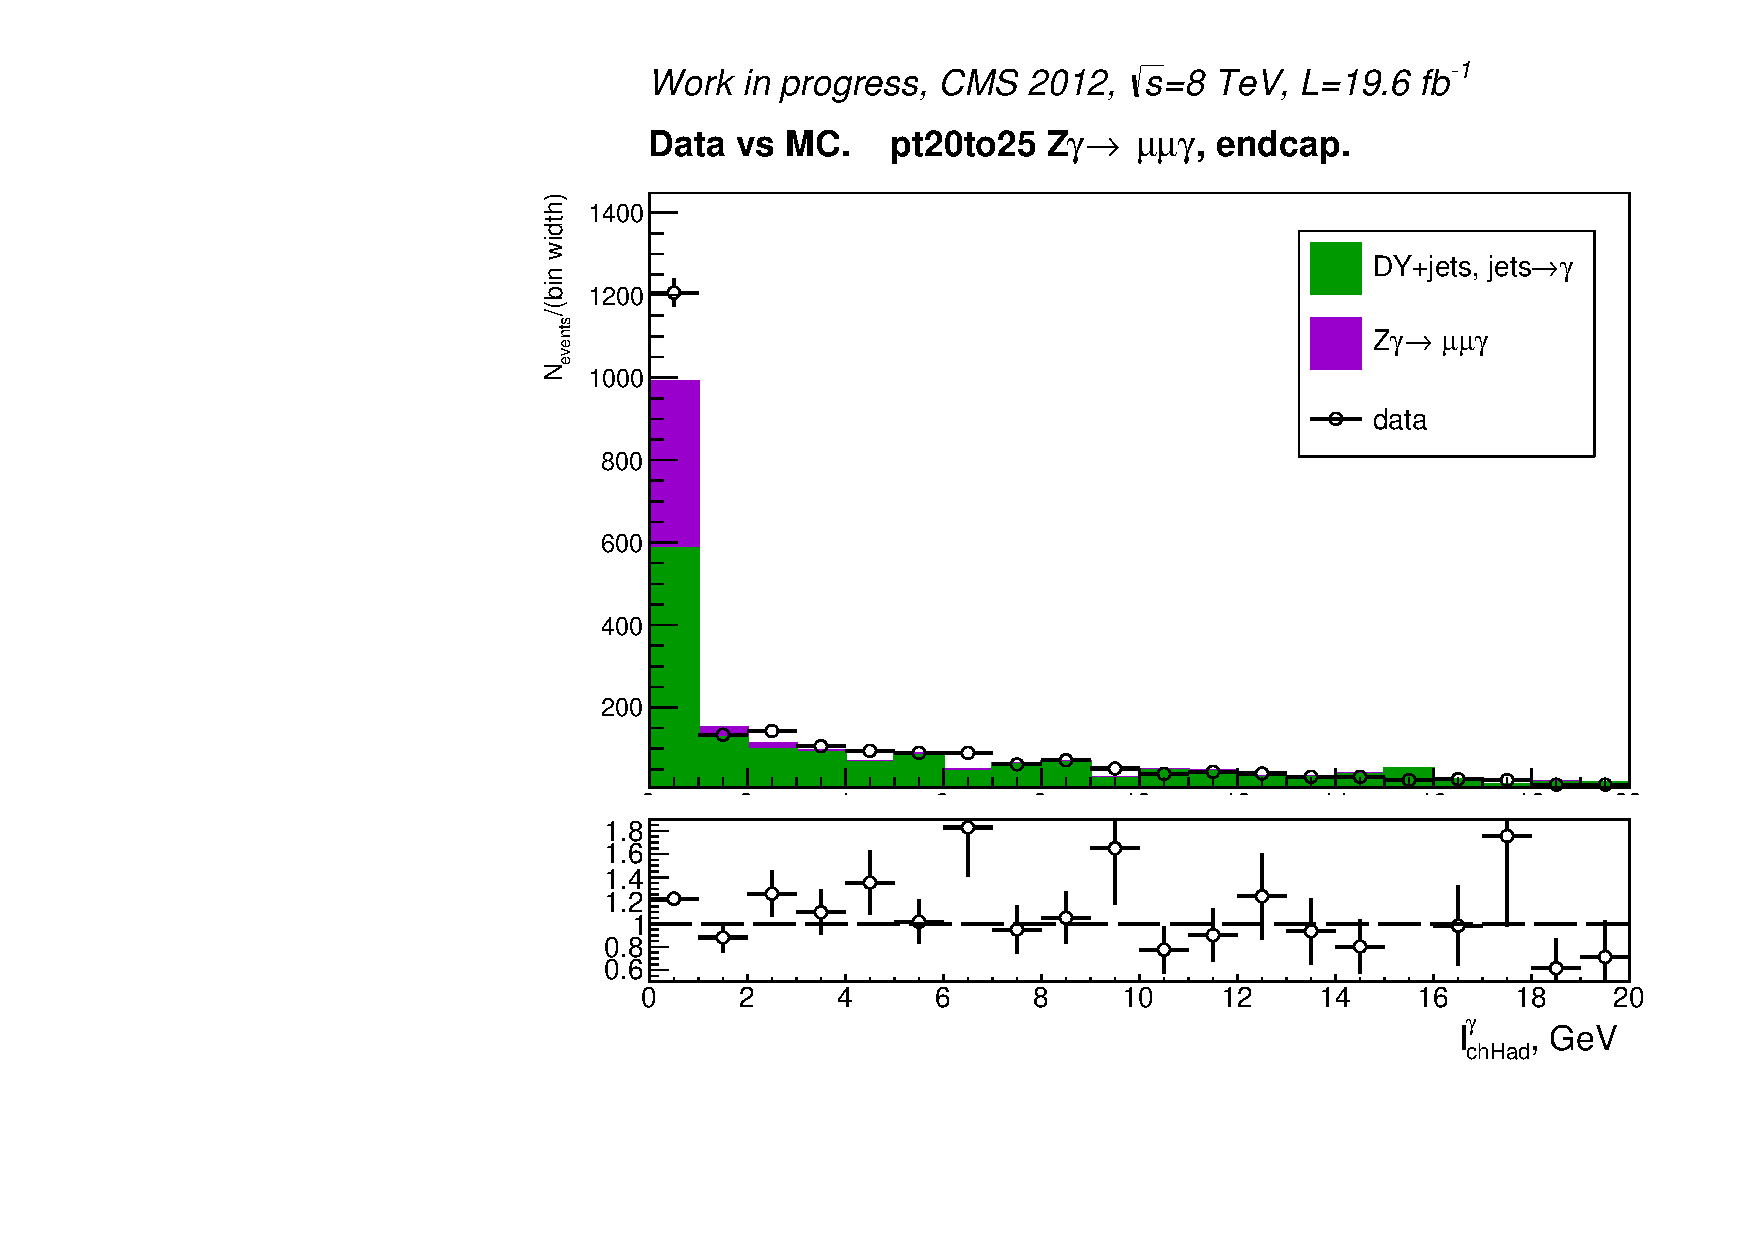
\includegraphics[width=0.32\textwidth]{../figs/figs_v11/MUON_ZGamma/PrepareYields/c_TotalDATAvsMC_Endcap__phoPFChIsoCorrFSR_EXCLUDED_pt20to25_.pdf}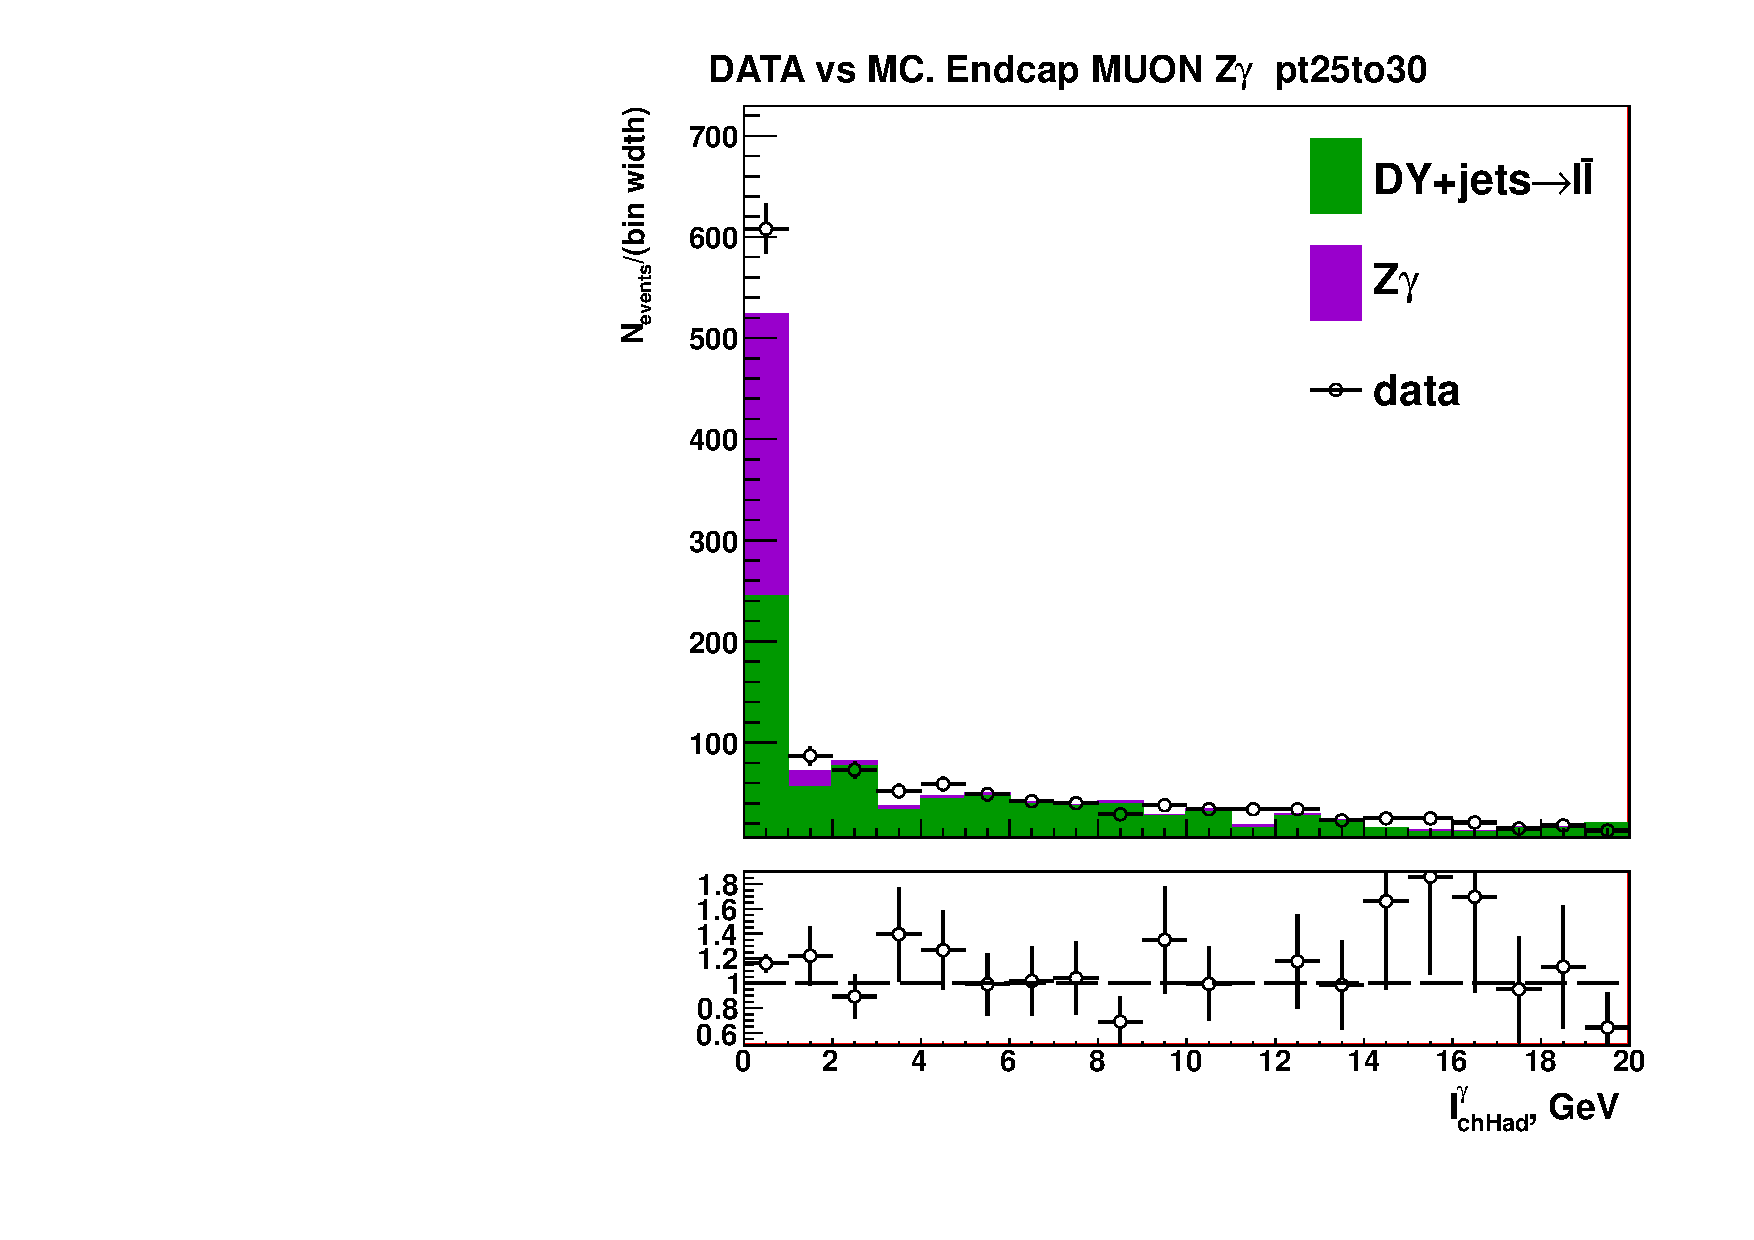
\includegraphics[width=0.32\textwidth]{../figs/figs_v11/MUON_ZGamma/PrepareYields/c_TotalDATAvsMC_Endcap__phoPFChIsoCorrFSR_EXCLUDED_pt25to30_.pdf}\\
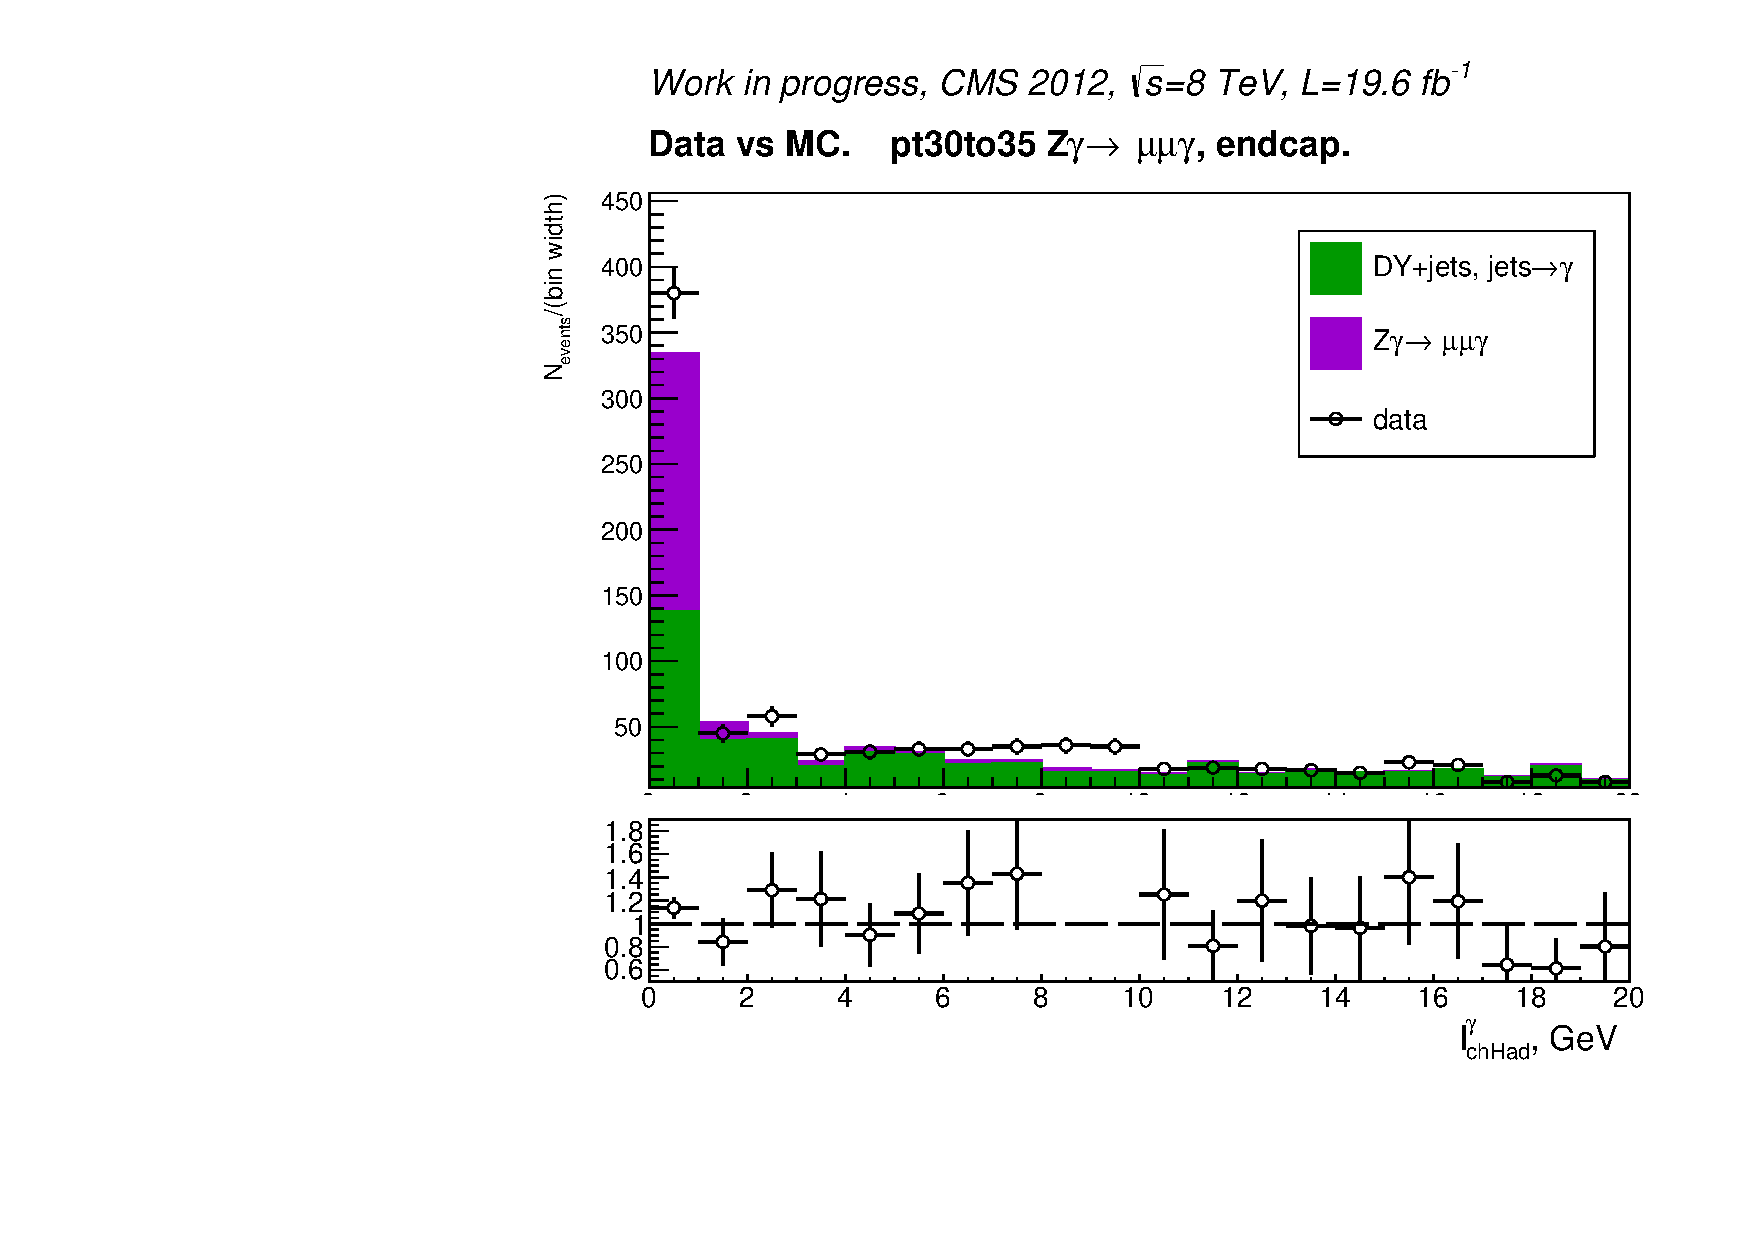
\includegraphics[width=0.32\textwidth]{../figs/figs_v11/MUON_ZGamma/PrepareYields/c_TotalDATAvsMC_Endcap__phoPFChIsoCorrFSR_EXCLUDED_pt30to35_.pdf}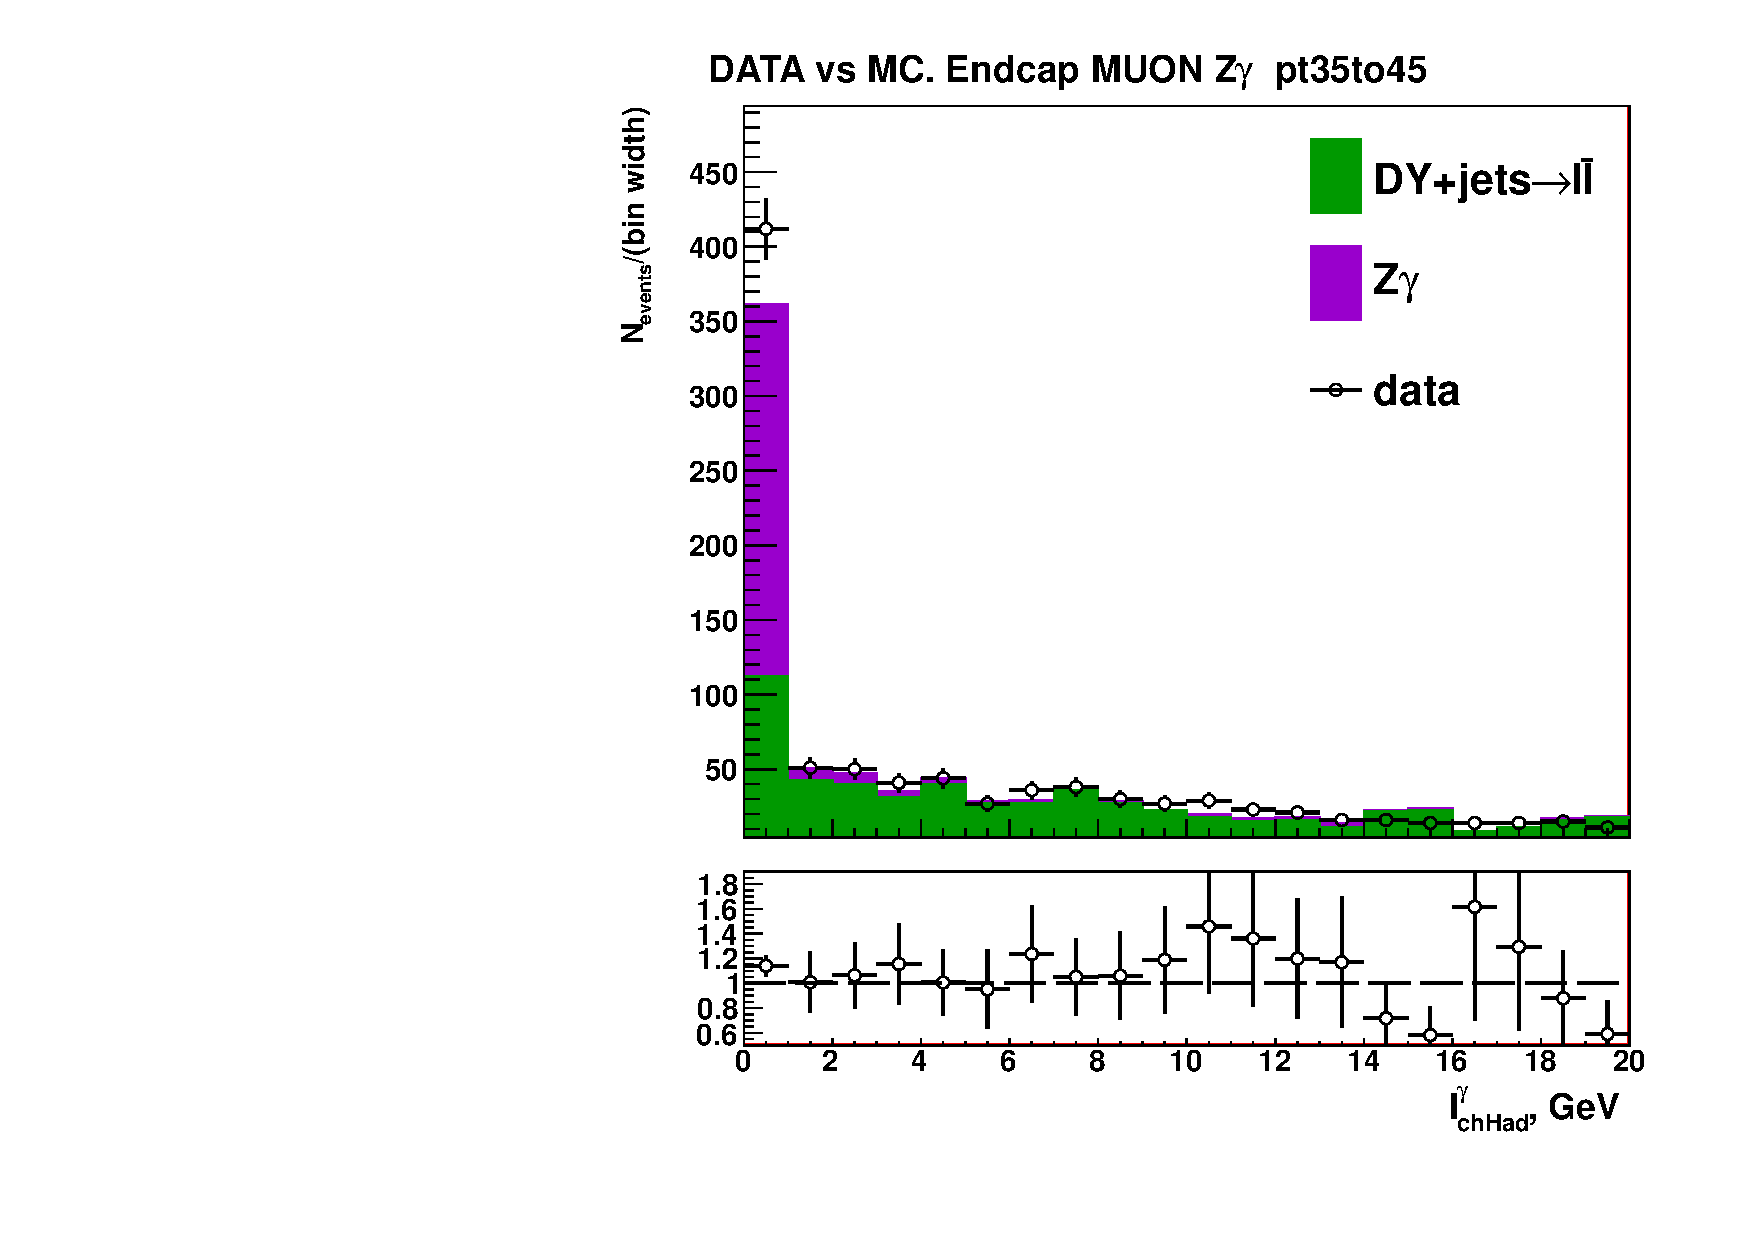
\includegraphics[width=0.32\textwidth]{../figs/figs_v11/MUON_ZGamma/PrepareYields/c_TotalDATAvsMC_Endcap__phoPFChIsoCorrFSR_EXCLUDED_pt35to45_.pdf}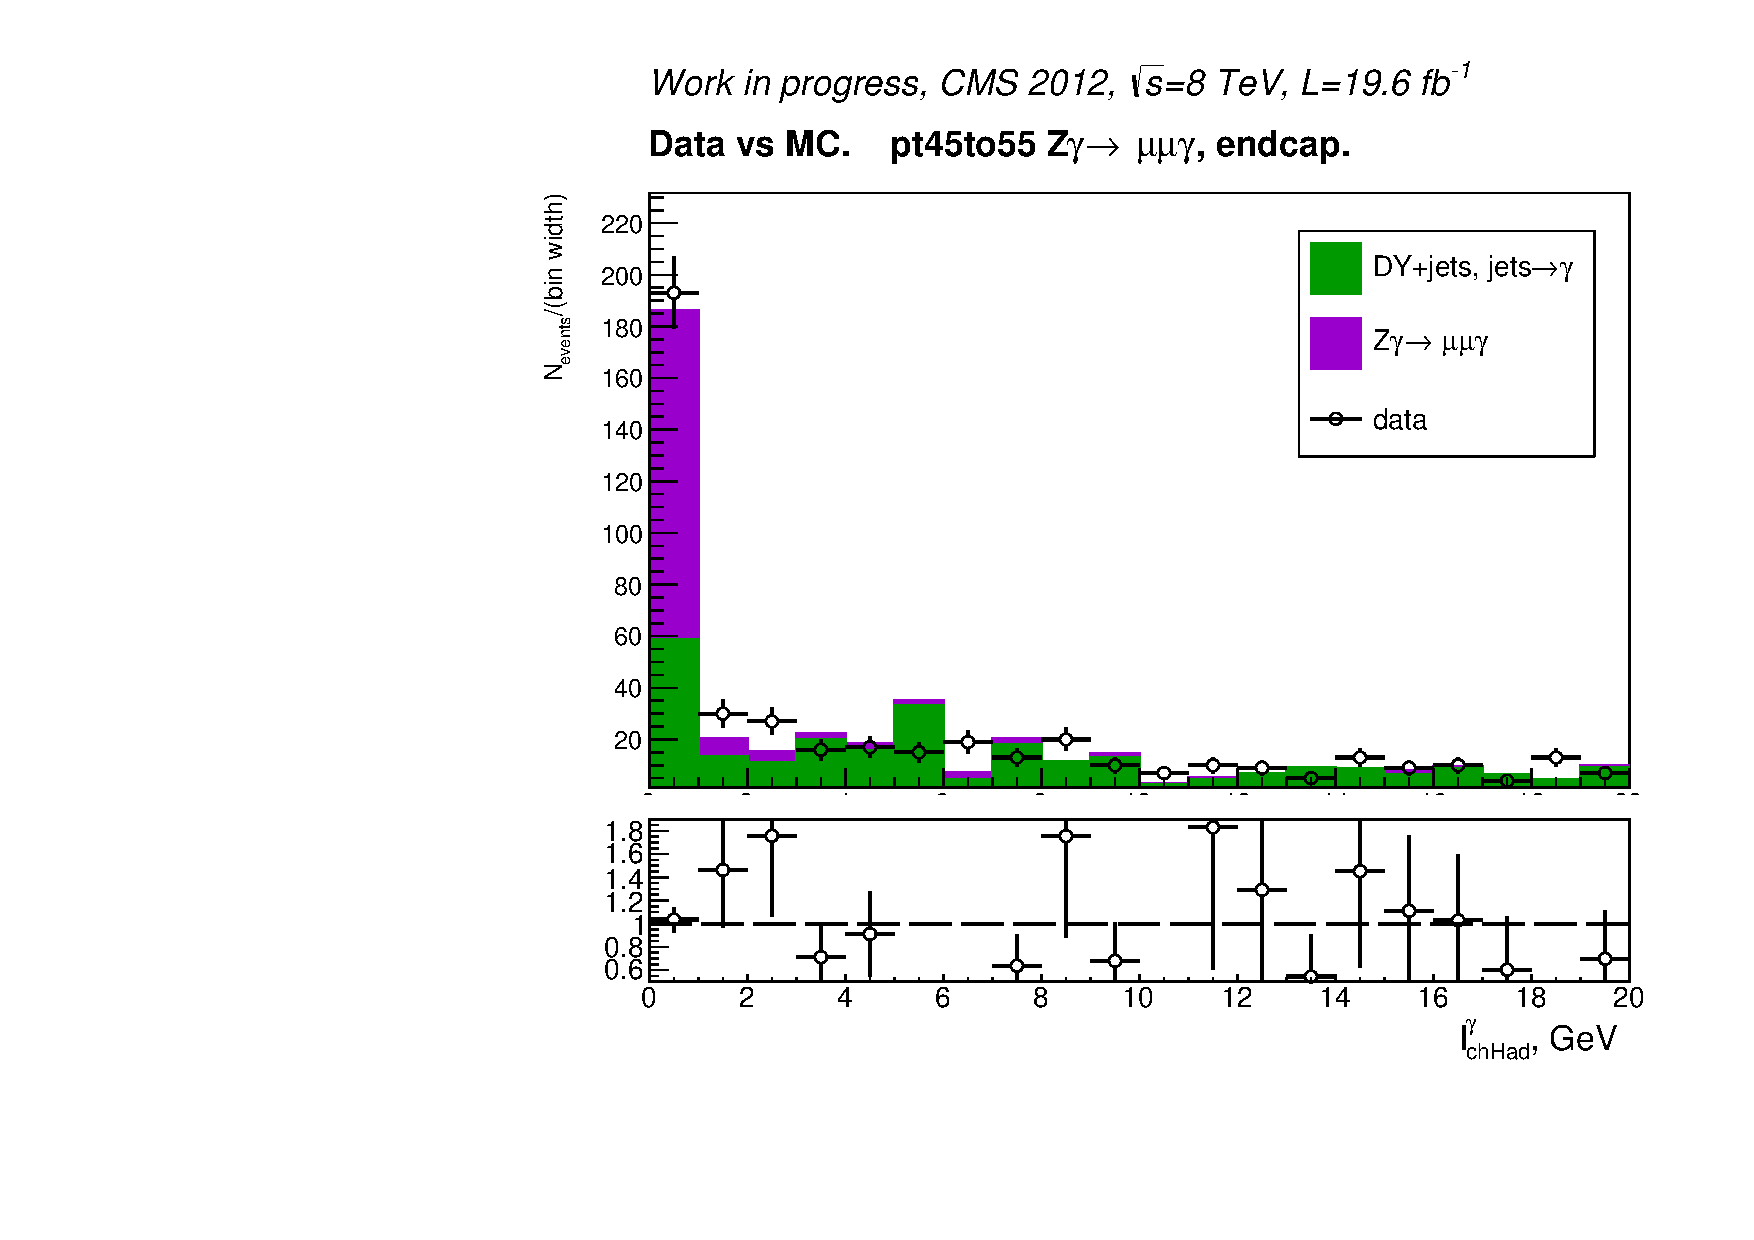
\includegraphics[width=0.32\textwidth]{../figs/figs_v11/MUON_ZGamma/PrepareYields/c_TotalDATAvsMC_Endcap__phoPFChIsoCorrFSR_EXCLUDED_pt45to55_.pdf}\\
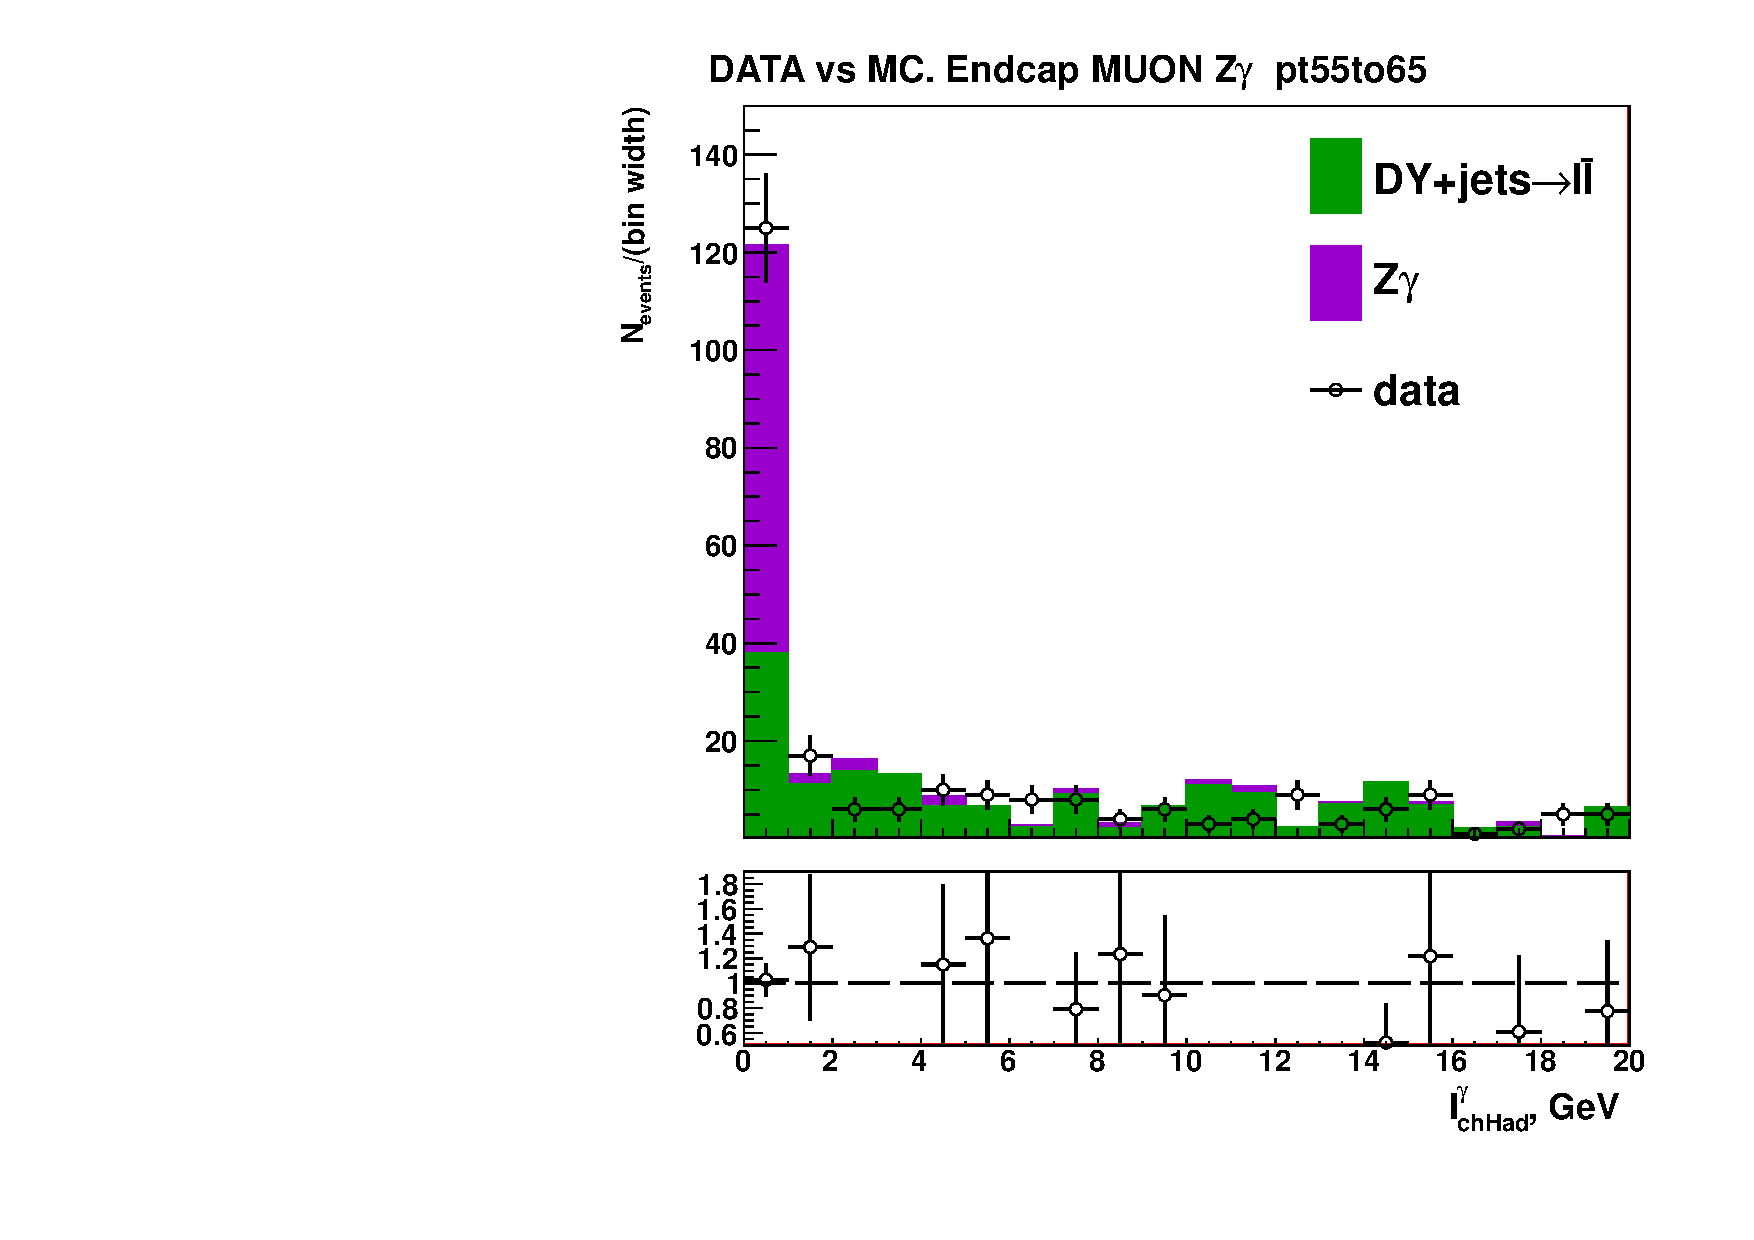
\includegraphics[width=0.32\textwidth]{../figs/figs_v11/MUON_ZGamma/PrepareYields/c_TotalDATAvsMC_Endcap__phoPFChIsoCorrFSR_EXCLUDED_pt55to65_.pdf}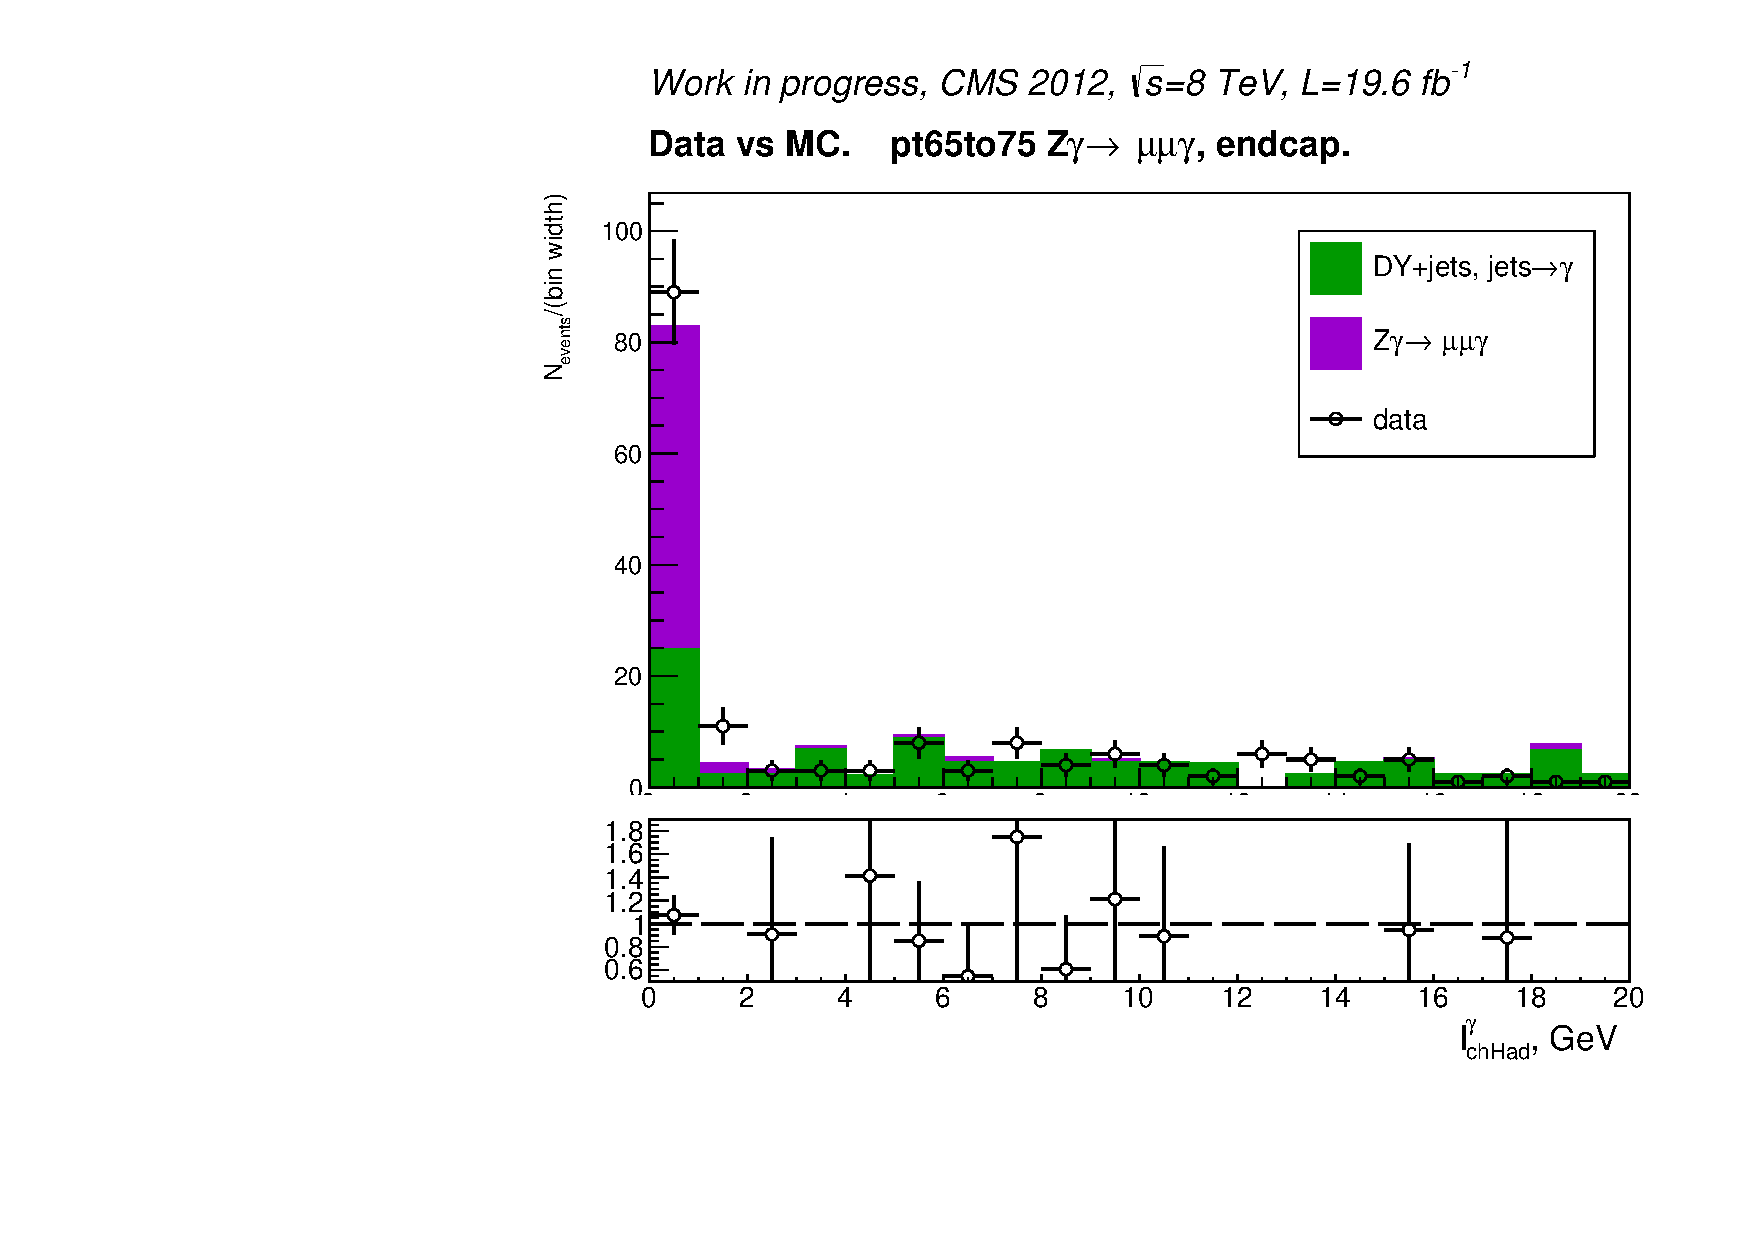
\includegraphics[width=0.32\textwidth]{../figs/figs_v11/MUON_ZGamma/PrepareYields/c_TotalDATAvsMC_Endcap__phoPFChIsoCorrFSR_EXCLUDED_pt65to75_.pdf}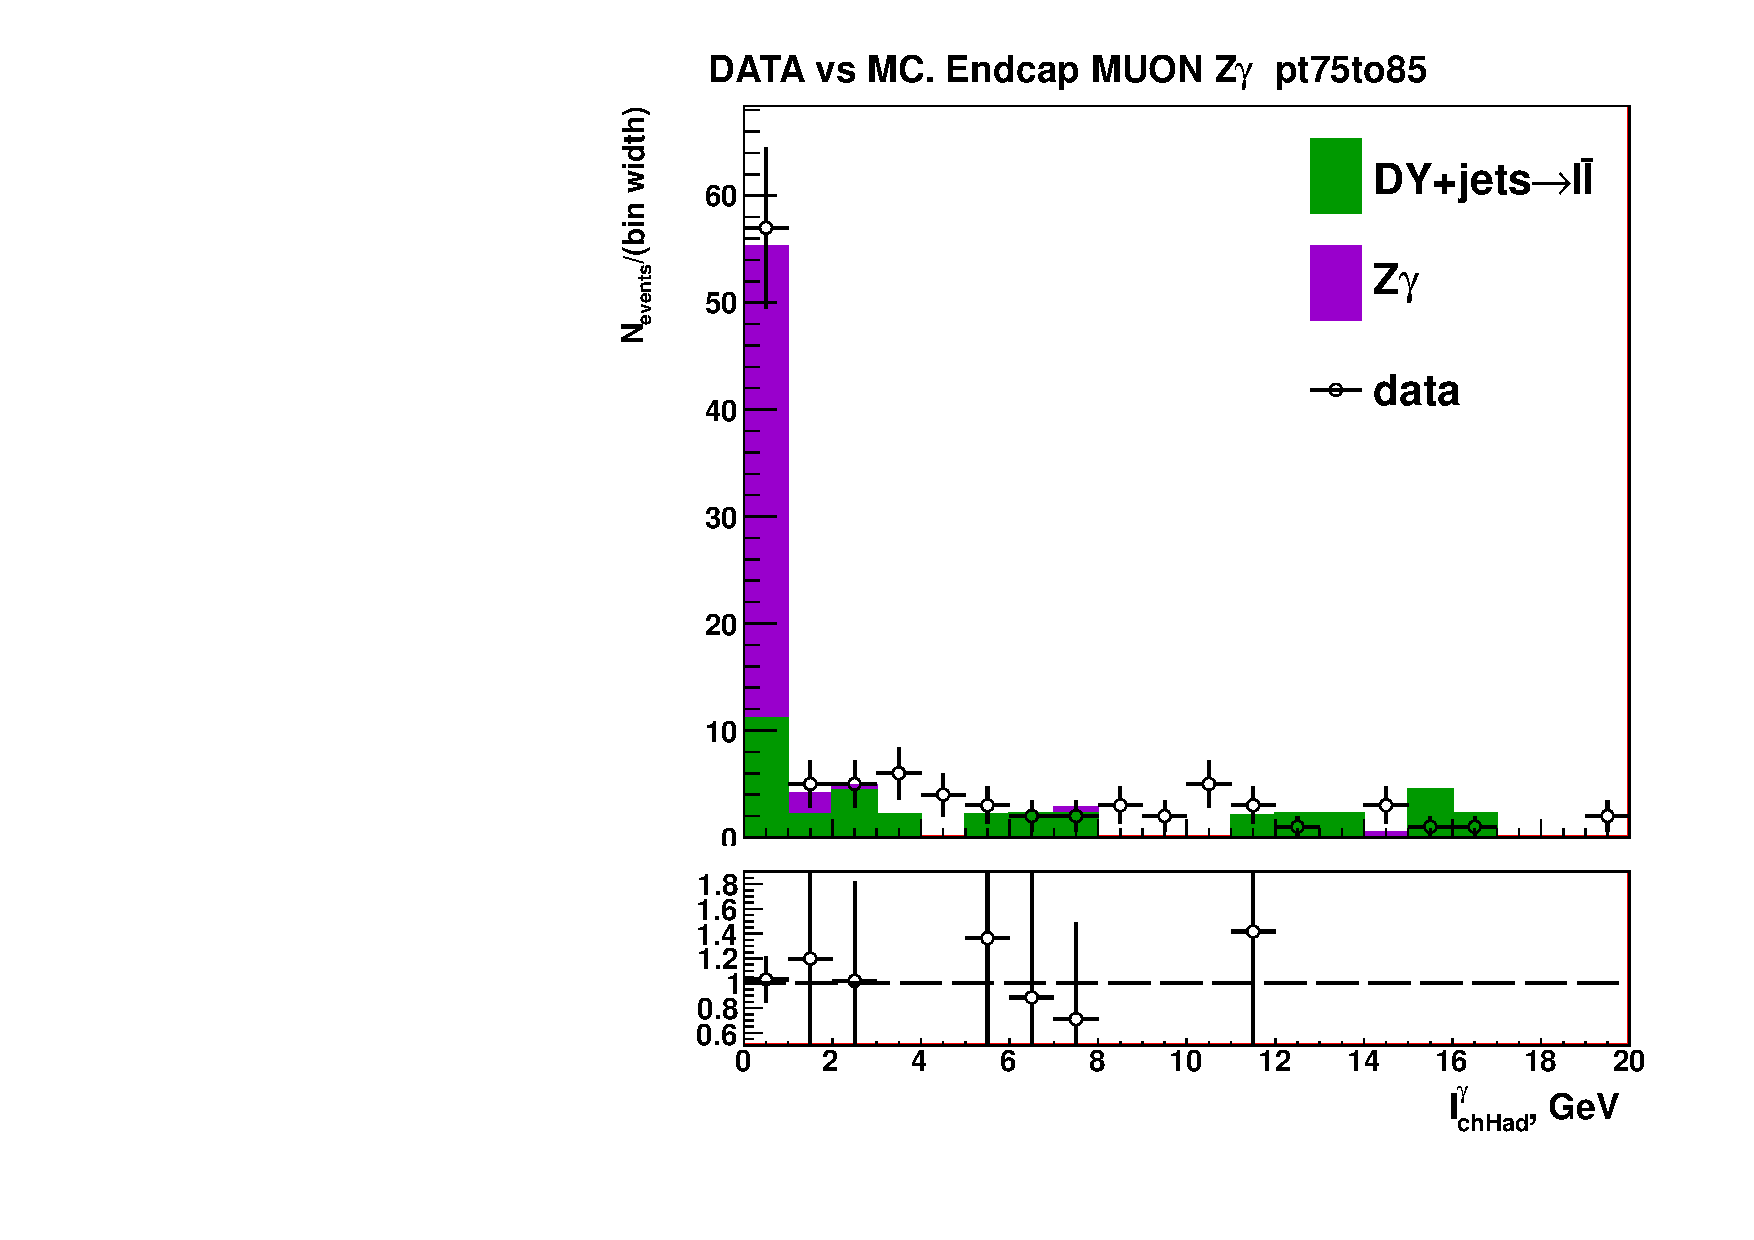
\includegraphics[width=0.32\textwidth]{../figs/figs_v11/MUON_ZGamma/PrepareYields/c_TotalDATAvsMC_Endcap__phoPFChIsoCorrFSR_EXCLUDED_pt75to85_.pdf}\\
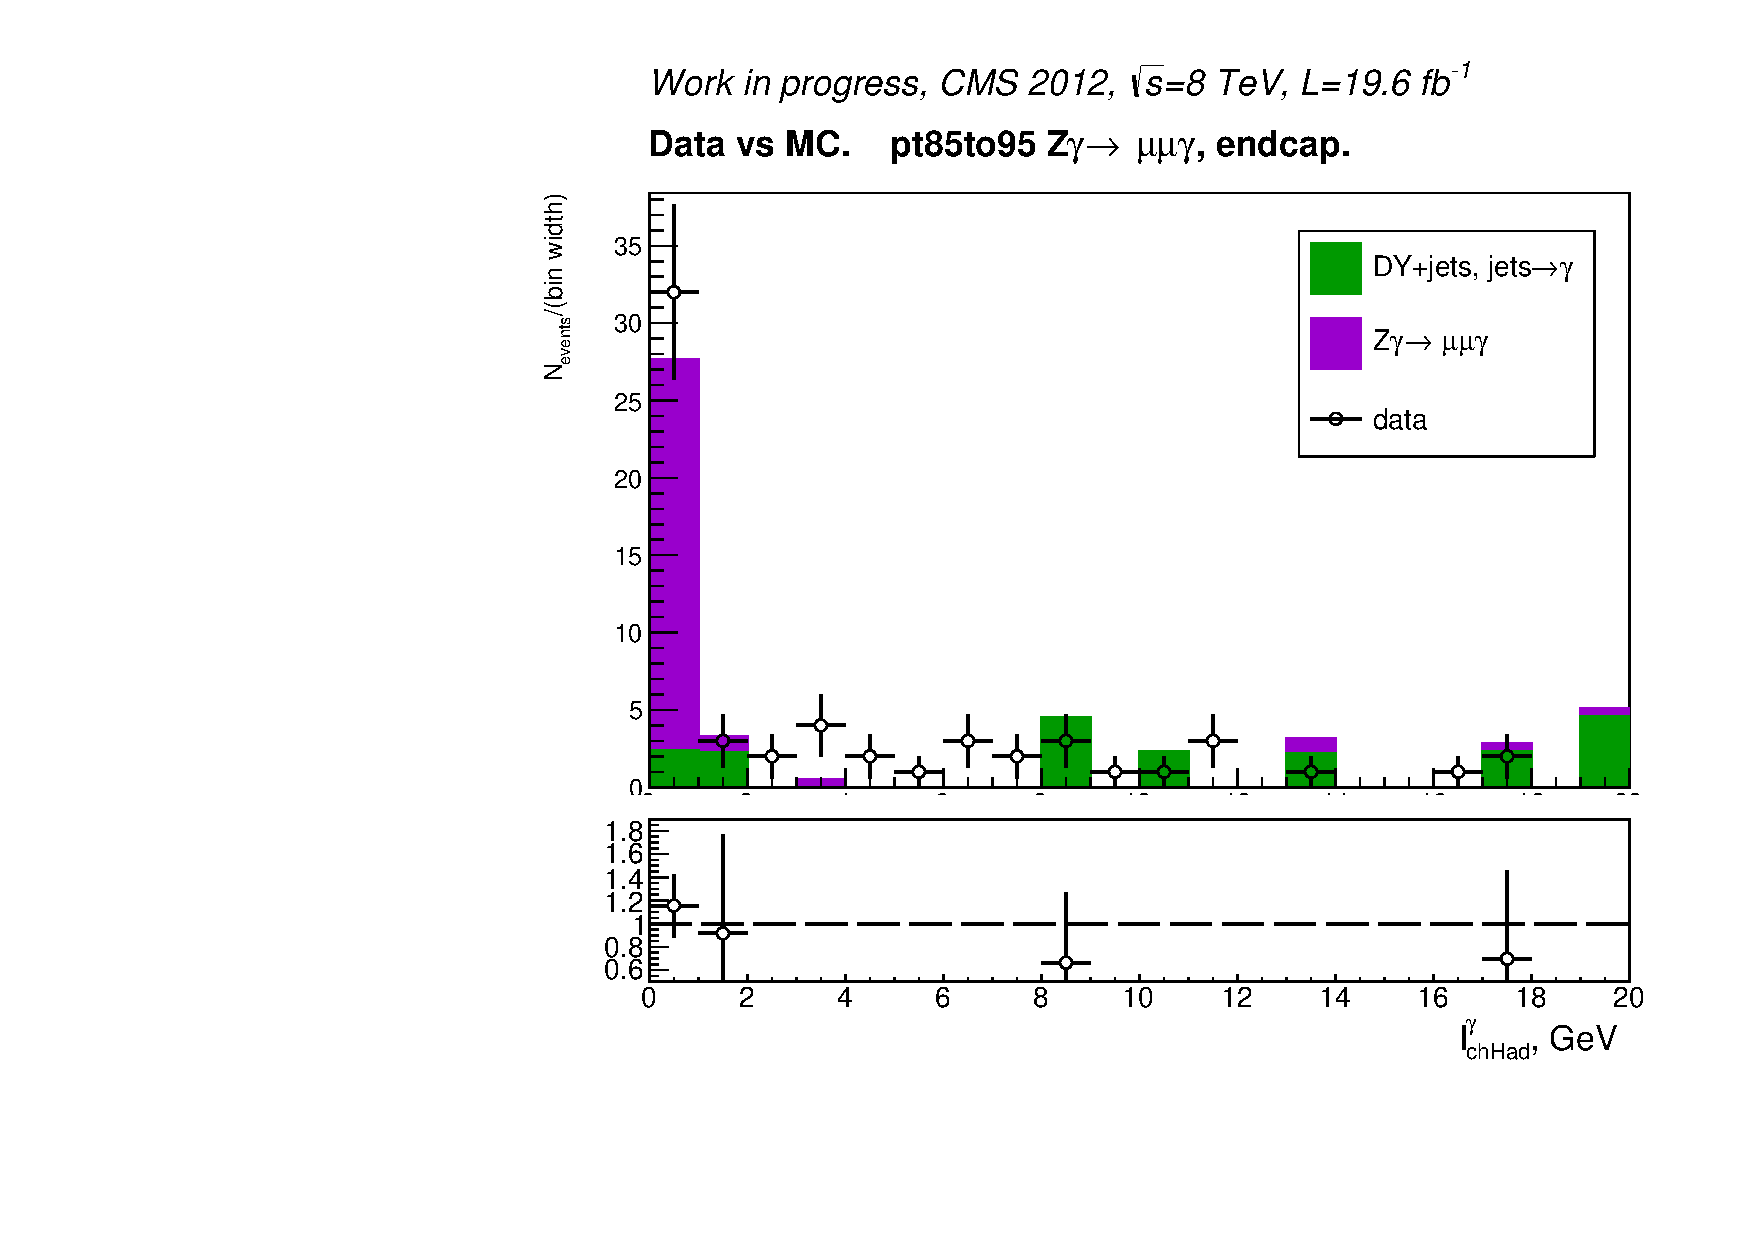
\includegraphics[width=0.32\textwidth]{../figs/figs_v11/MUON_ZGamma/PrepareYields/c_TotalDATAvsMC_Endcap__phoPFChIsoCorrFSR_EXCLUDED_pt85to95_.pdf}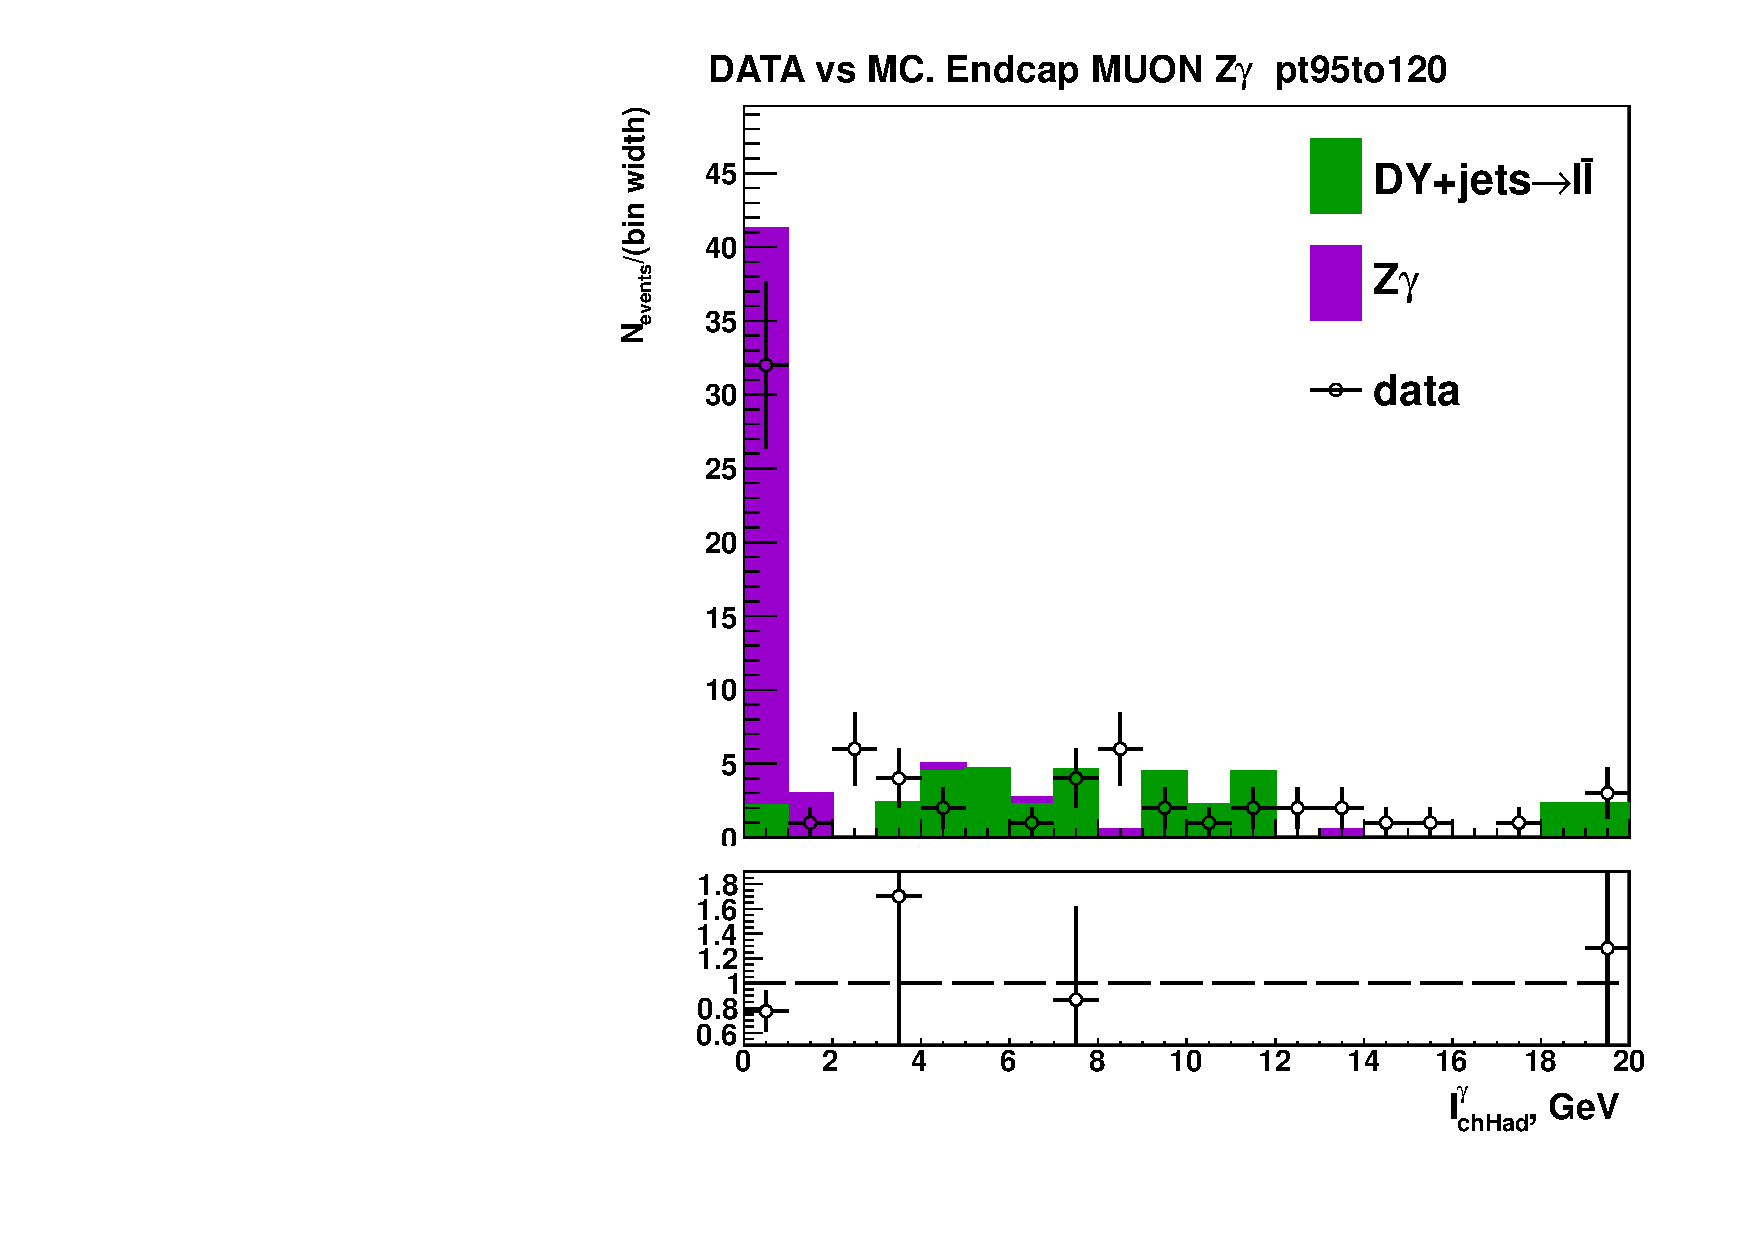
\includegraphics[width=0.32\textwidth]{../figs/figs_v11/MUON_ZGamma/PrepareYields/c_TotalDATAvsMC_Endcap__phoPFChIsoCorrFSR_EXCLUDED_pt95to120_.pdf}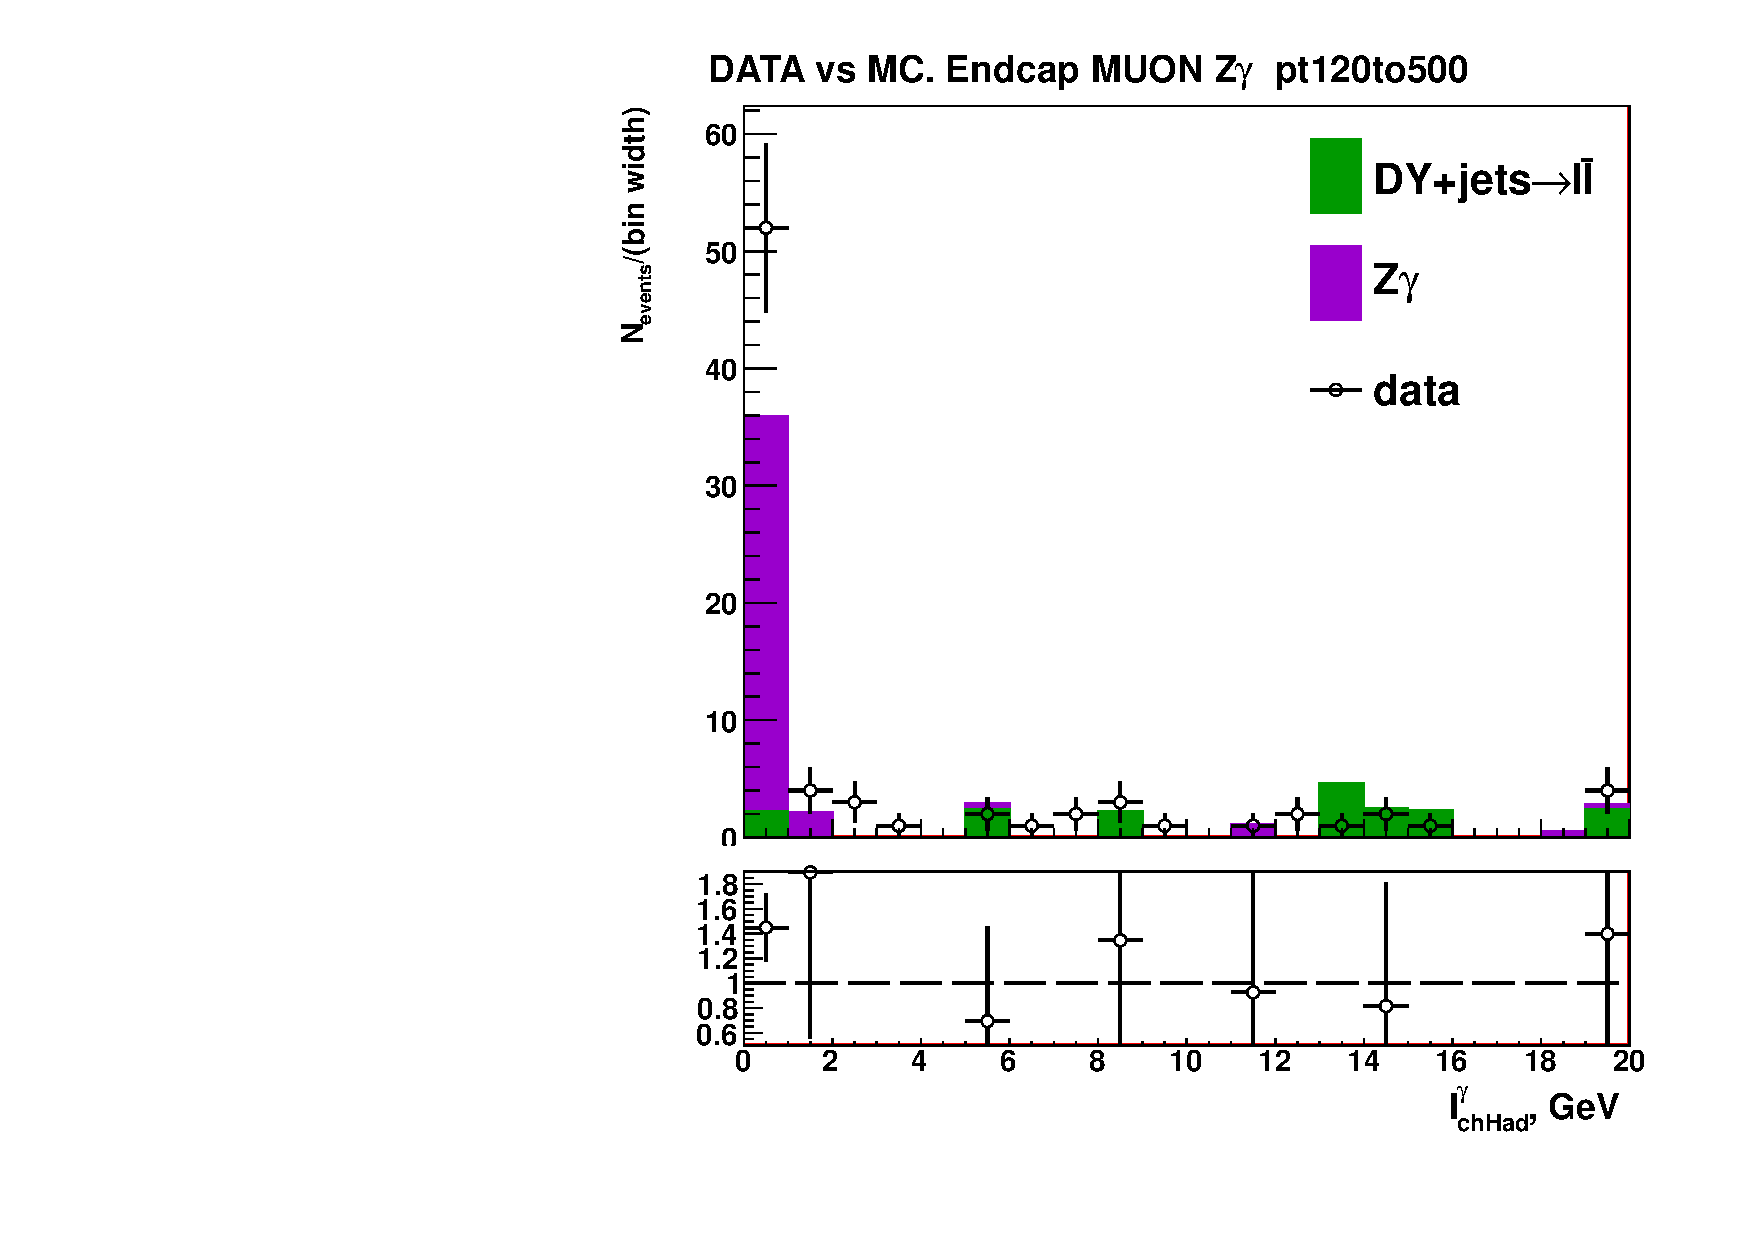
\includegraphics[width=0.32\textwidth]{../figs/figs_v11/MUON_ZGamma/PrepareYields/c_TotalDATAvsMC_Endcap__phoPFChIsoCorrFSR_EXCLUDED_pt120to500_.pdf}\\
  \caption{$Z\gamma$-selected ISR events, data vs MC. $15$~GeV$<P_T^{\gamma}<500$~GeV, Endcap photons. Distributions of $I_{chHad}^{\gamma}$ used for preparing fake-$\gamma$ templates. Real-$\gamma$ contribution to ISR region is subtracted based on $Z\gamma$ signal MC prediction to prepare fake-$\gamma$ templates.}
  \label{fig:Zg_ISR_phoPFChIsoCorr_Endcap}
  \end{center}
\end{figure}

\begin{figure}[htb]
  \begin{center}
   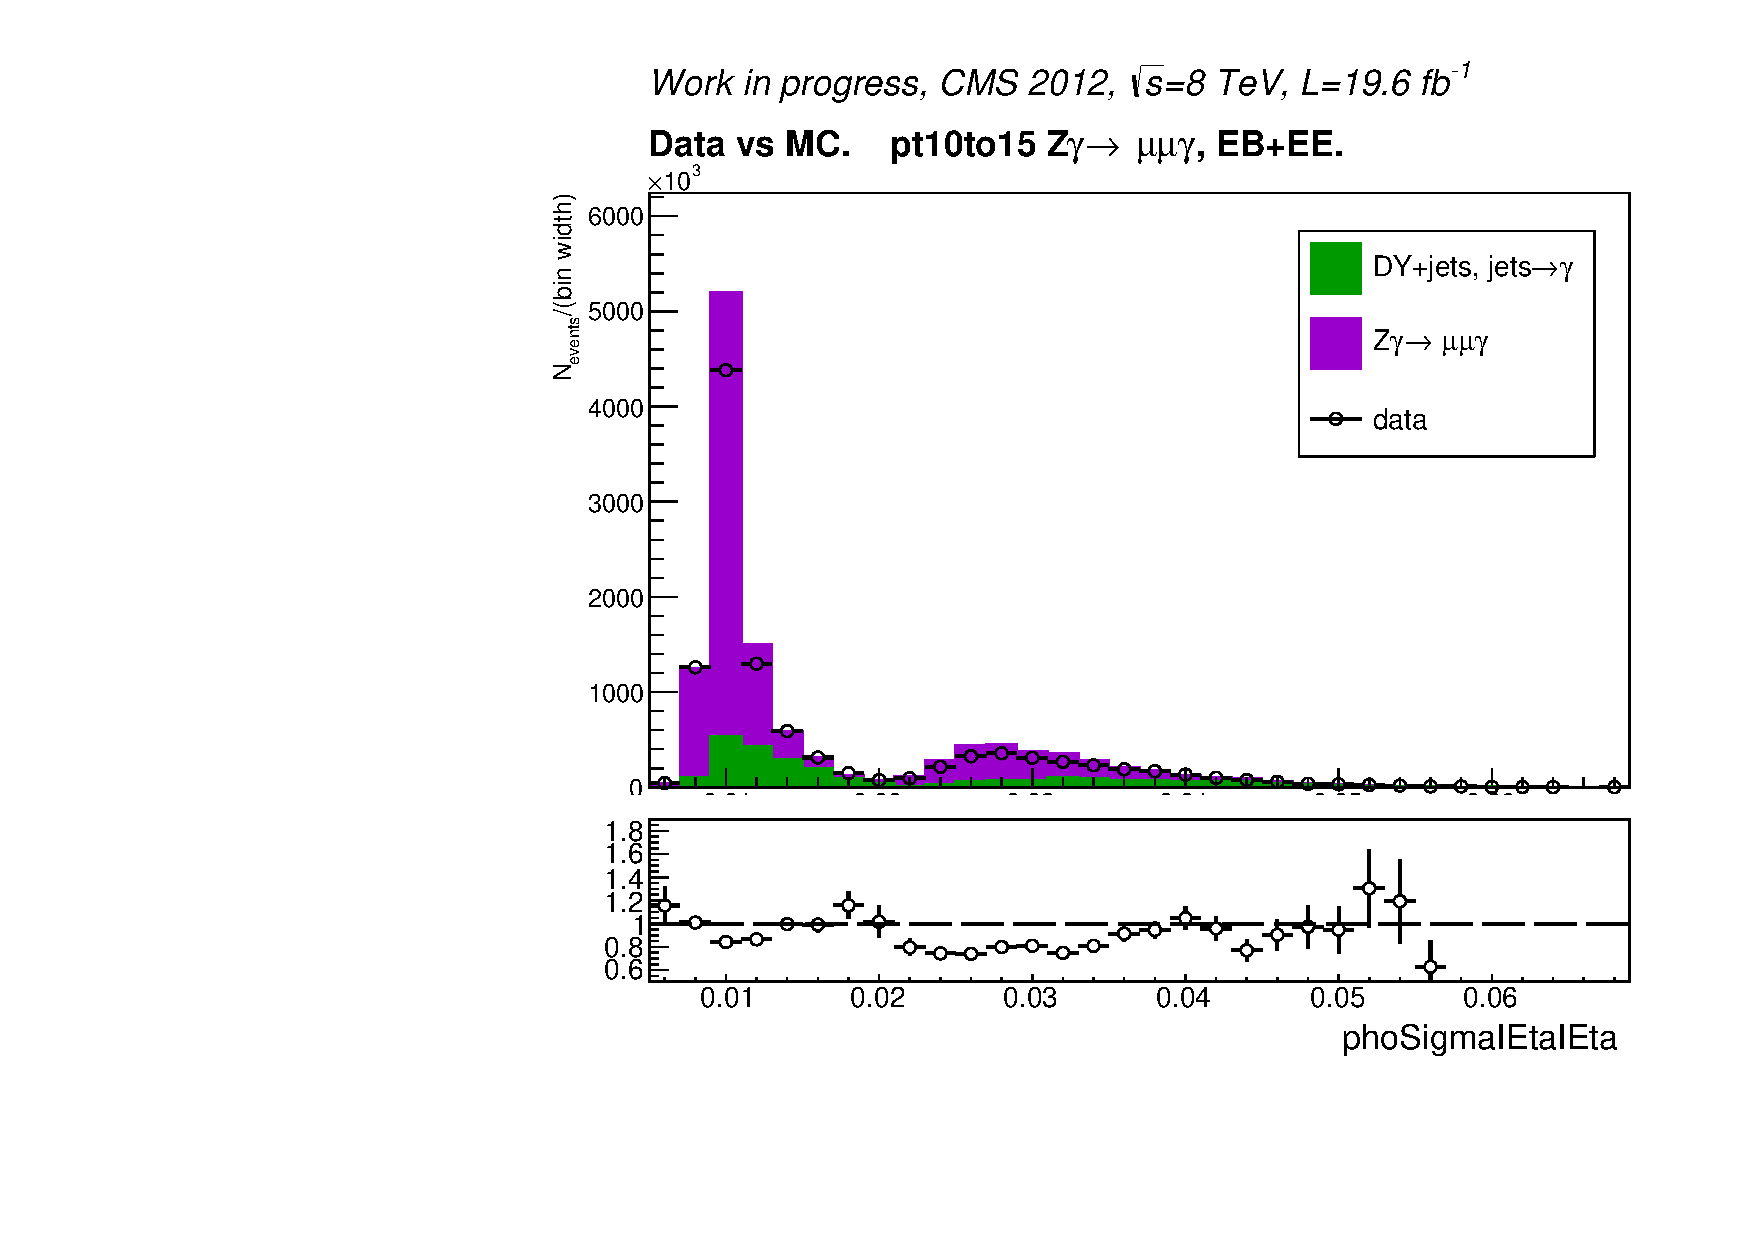
\includegraphics[width=0.45\textwidth]{../figs/figs_v11/MUON_ZGamma/PrepareYields/c_TotalDATAvsMC_EtaCommon__phoSigmaIEtaIEtaFSR_pt10to15_.pdf}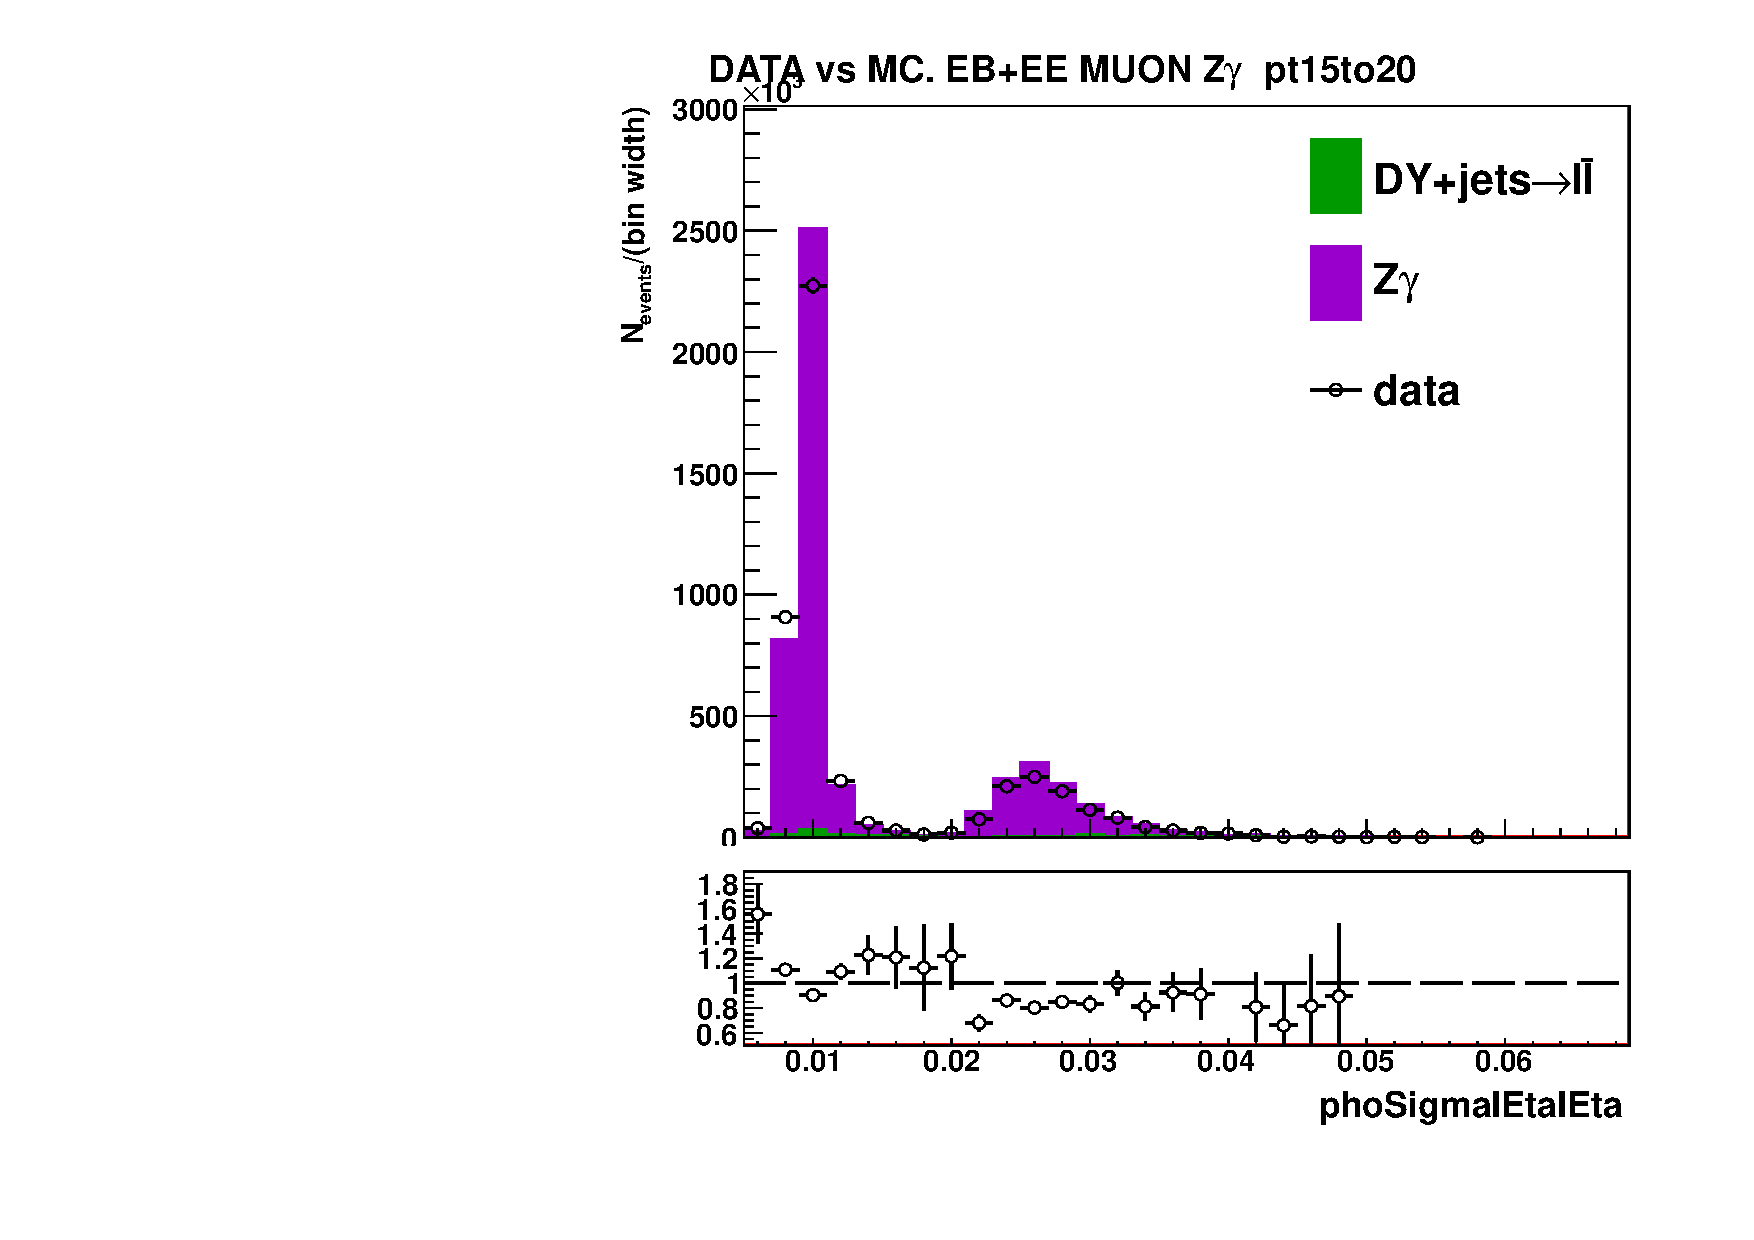
\includegraphics[width=0.45\textwidth]{../figs/figs_v11/MUON_ZGamma/PrepareYields/c_TotalDATAvsMC_EtaCommon__phoSigmaIEtaIEtaFSR_pt15to20_.pdf}\\
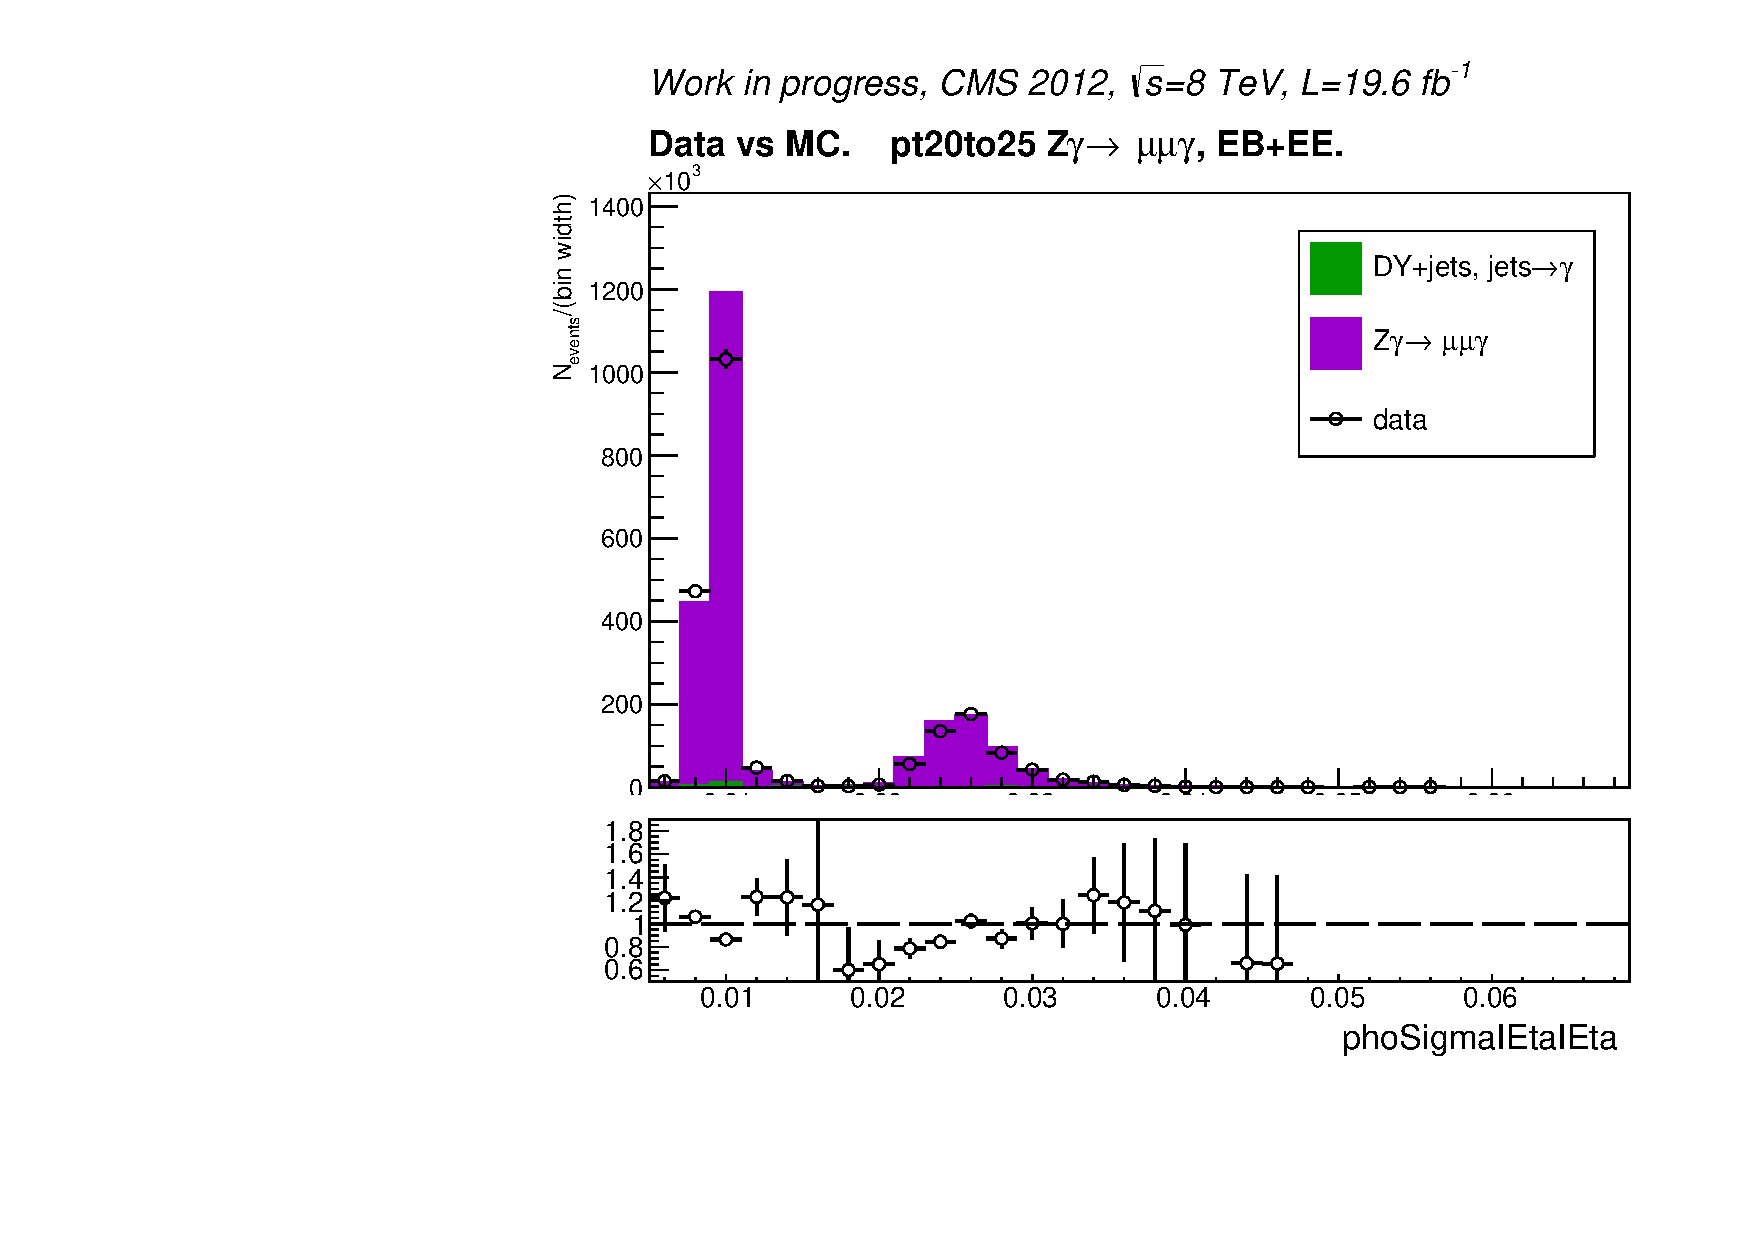
\includegraphics[width=0.32\textwidth]{../figs/figs_v11/MUON_ZGamma/PrepareYields/c_TotalDATAvsMC_EtaCommon__phoSigmaIEtaIEtaFSR_pt20to25_.pdf}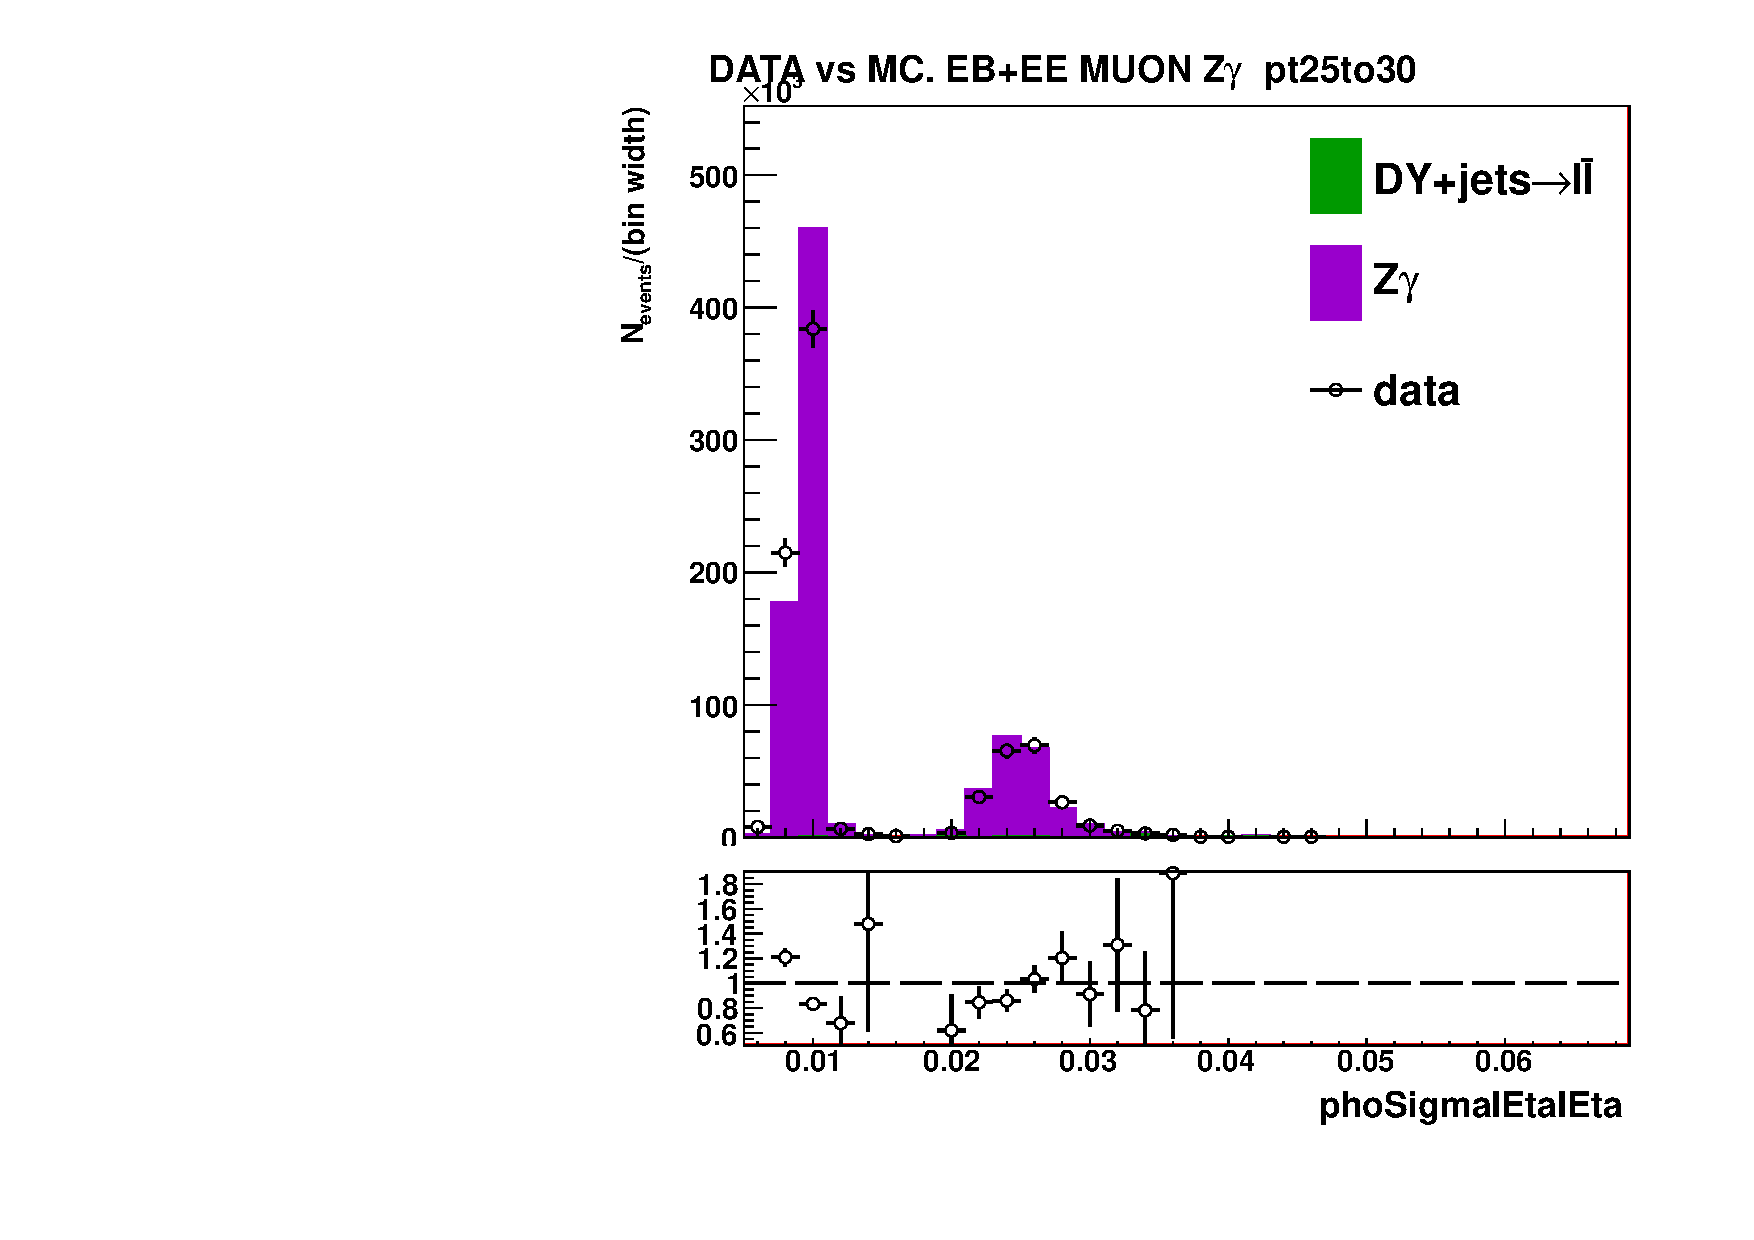
\includegraphics[width=0.32\textwidth]{../figs/figs_v11/MUON_ZGamma/PrepareYields/c_TotalDATAvsMC_EtaCommon__phoSigmaIEtaIEtaFSR_pt25to30_.pdf}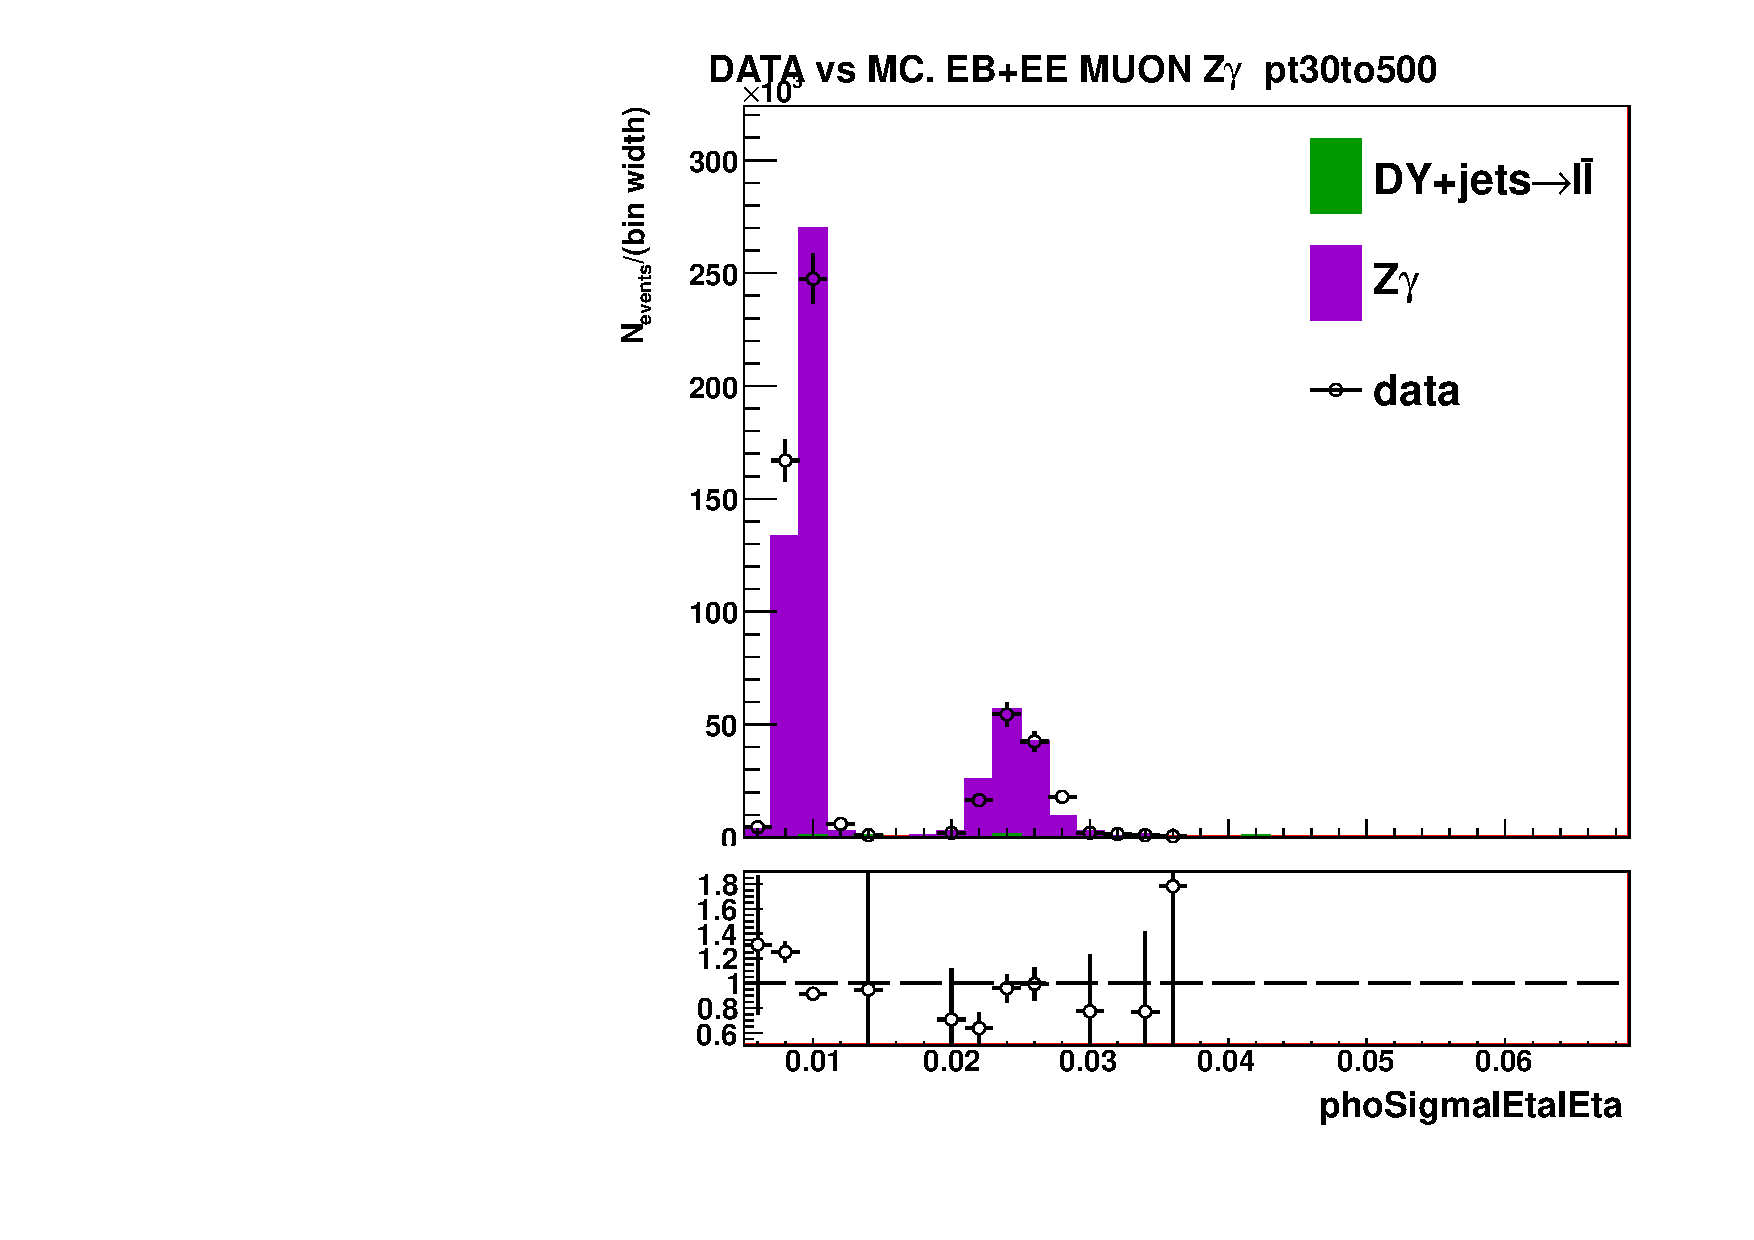
\includegraphics[width=0.32\textwidth]{../figs/figs_v11/MUON_ZGamma/PrepareYields/c_TotalDATAvsMC_EtaCommon__phoSigmaIEtaIEtaFSR_pt30to500_.pdf}\\
  \caption{$Z\gamma$-selected FSR events, data vs MC. Distributions of $\sigma_{i\eta i \eta}$ are used for preparing real-$\gamma$ templates. Fake-$\gamma$ contribution to FSR region is subtracted based on DY+jets MC prediction to prepare real-$\gamma$ templates. The templates are prepared separately for barrel and endcap photons.}
  \label{fig:Zg_FSR_phoSigmaIEtaIEta}
  \end{center}
\end{figure}

\begin{figure}[htb]
  \begin{center}
   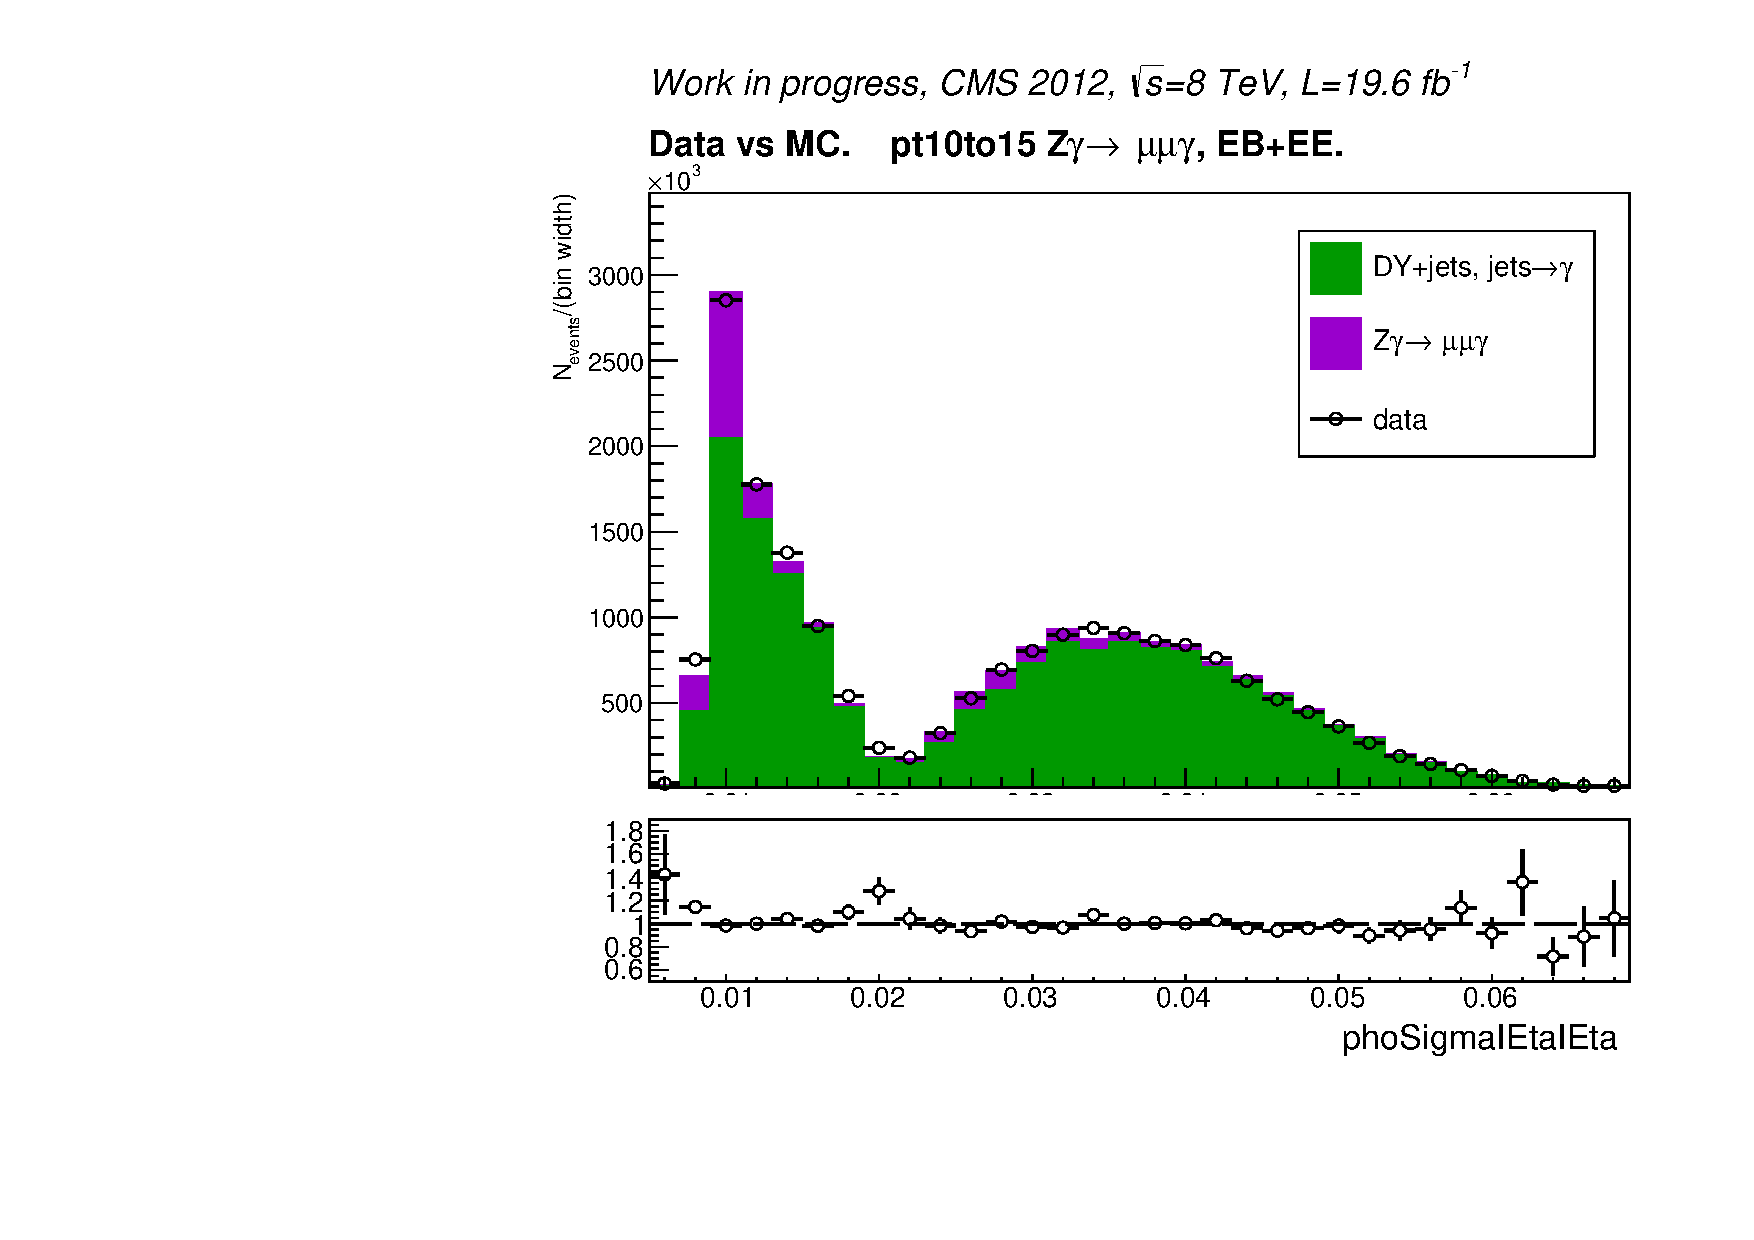
\includegraphics[width=0.45\textwidth]{../figs/figs_v11/MUON_ZGamma/PrepareYields/c_TotalDATAvsMC_EtaCommon__phoSigmaIEtaIEtaFSR_EXCLUDED_pt10to15_.pdf}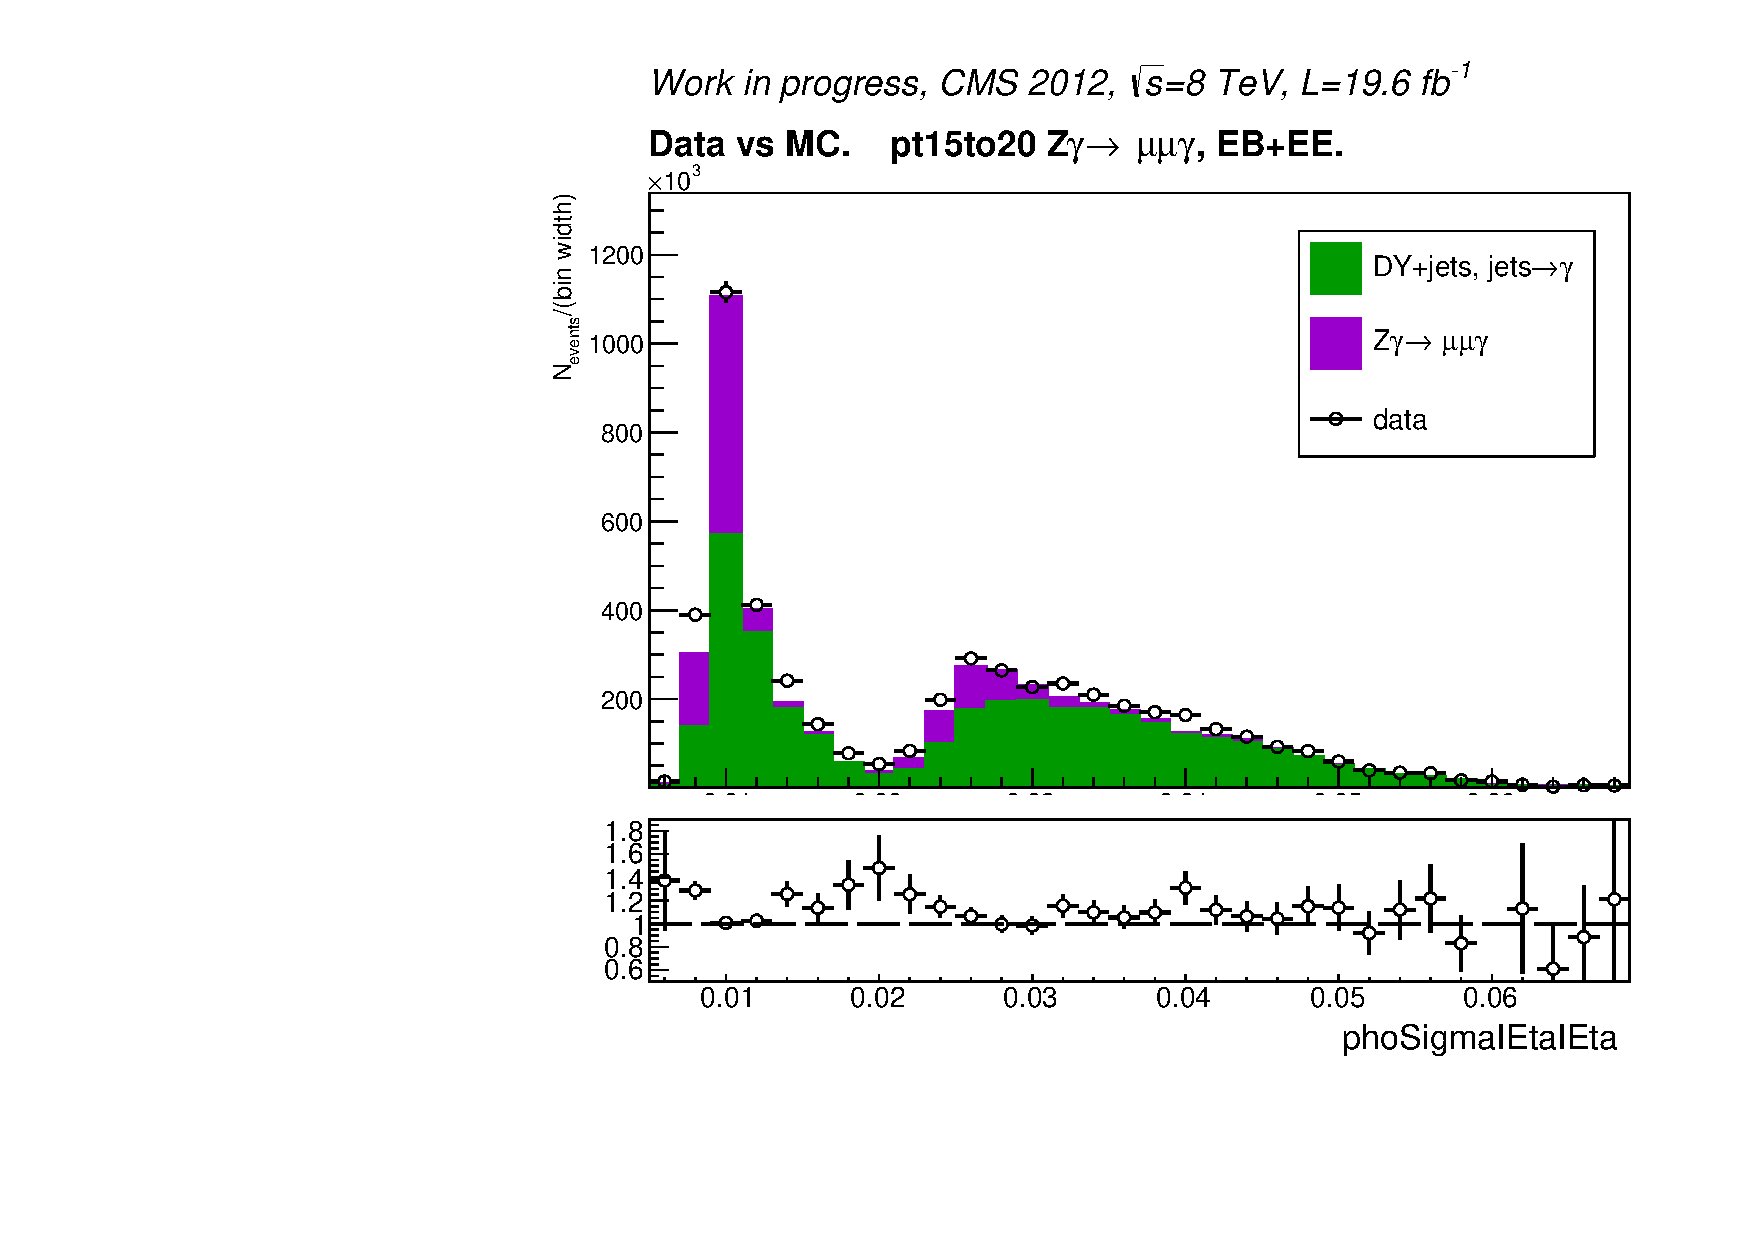
\includegraphics[width=0.45\textwidth]{../figs/figs_v11/MUON_ZGamma/PrepareYields/c_TotalDATAvsMC_EtaCommon__phoSigmaIEtaIEtaFSR_EXCLUDED_pt15to20_.pdf}\\
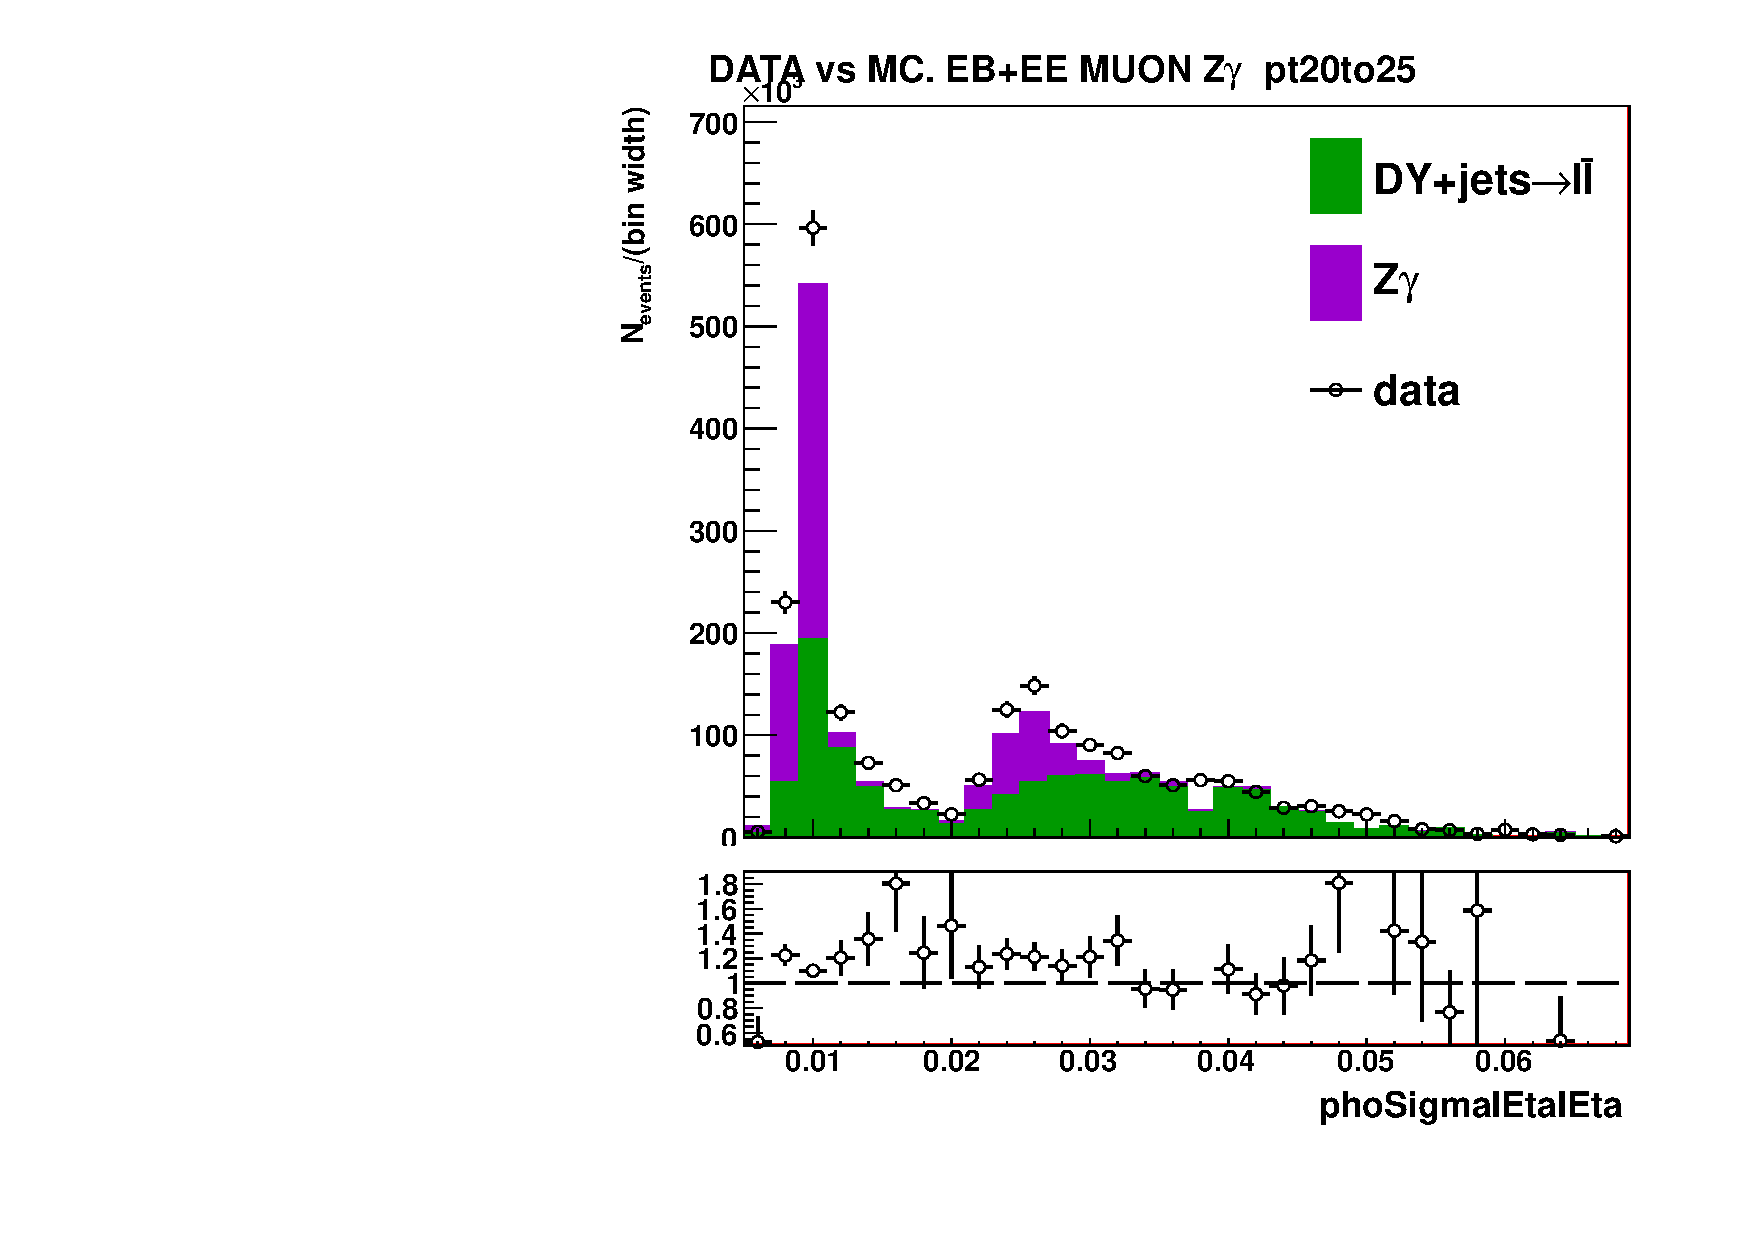
\includegraphics[width=0.32\textwidth]{../figs/figs_v11/MUON_ZGamma/PrepareYields/c_TotalDATAvsMC_EtaCommon__phoSigmaIEtaIEtaFSR_EXCLUDED_pt20to25_.pdf}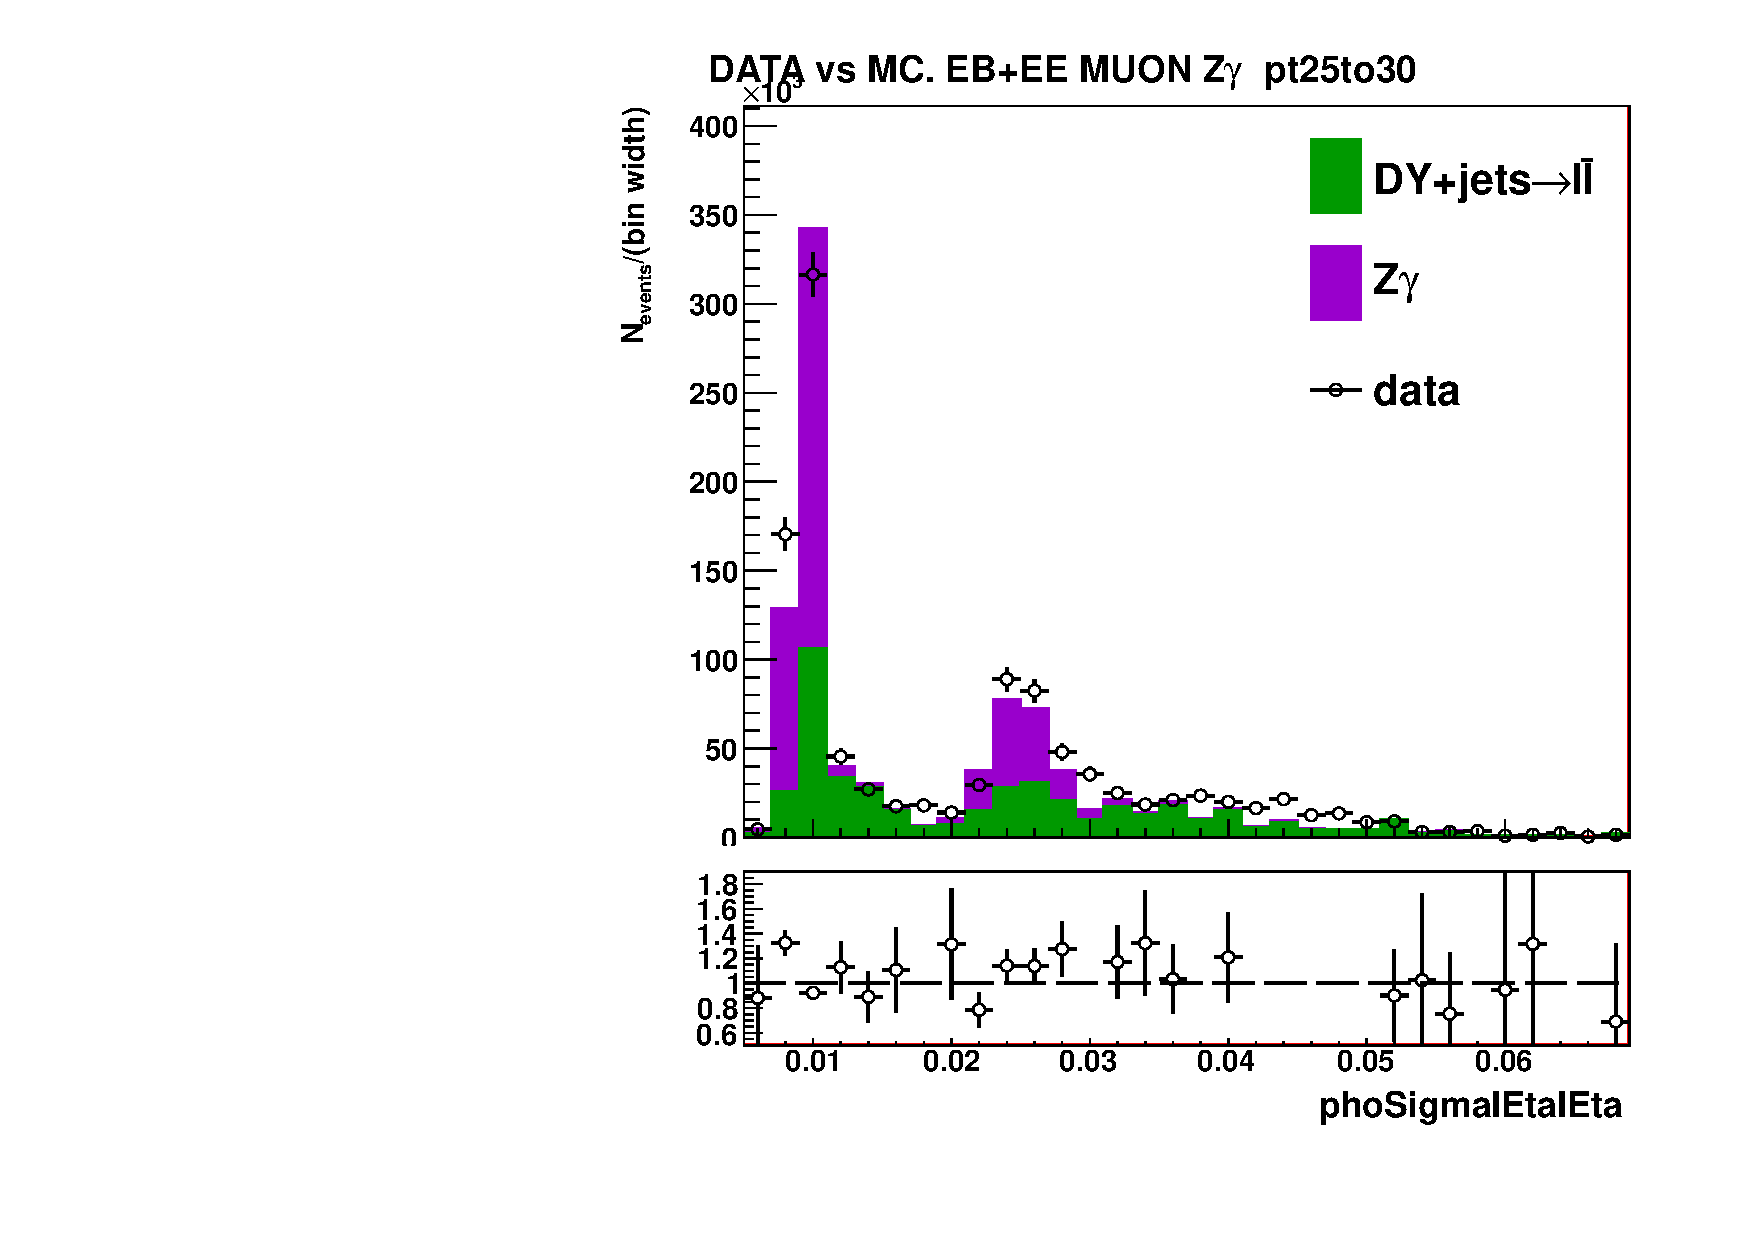
\includegraphics[width=0.32\textwidth]{../figs/figs_v11/MUON_ZGamma/PrepareYields/c_TotalDATAvsMC_EtaCommon__phoSigmaIEtaIEtaFSR_EXCLUDED_pt25to30_.pdf}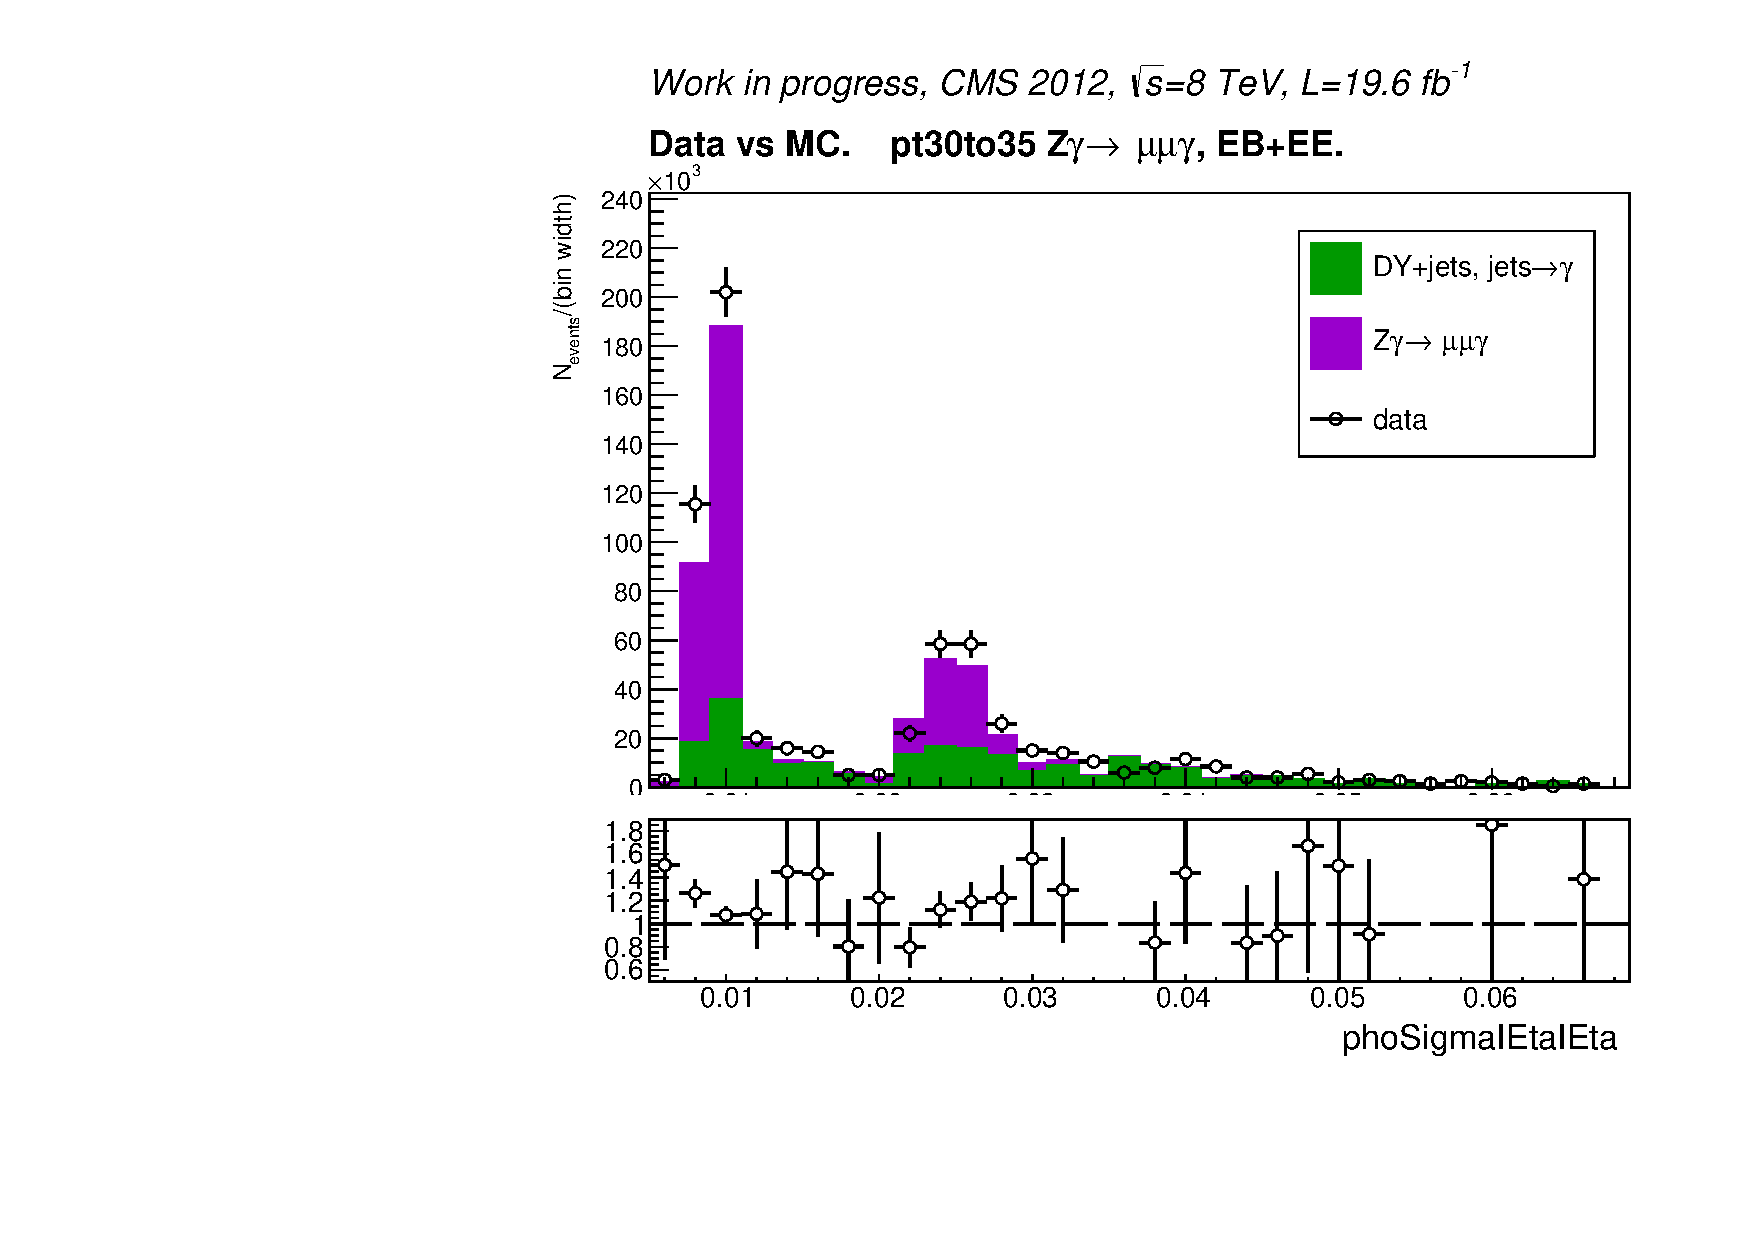
\includegraphics[width=0.32\textwidth]{../figs/figs_v11/MUON_ZGamma/PrepareYields/c_TotalDATAvsMC_EtaCommon__phoSigmaIEtaIEtaFSR_EXCLUDED_pt30to35_.pdf}\\
\includegraphics[width=0.32\textwidth]{../figs/figs_v11/MUON_ZGamma/PrepareYields/c_TotalDATAvsMC_EtaCommon__phoSigmaIEtaIEtaFSR_EXCLUDED_pt35to45_.pdf}\includegraphics[width=0.32\textwidth]{../figs/figs_v11/MUON_ZGamma/PrepareYields/c_TotalDATAvsMC_EtaCommon__phoSigmaIEtaIEtaFSR_EXCLUDED_pt45to55_.pdf}\includegraphics[width=0.32\textwidth]{../figs/figs_v11/MUON_ZGamma/PrepareYields/c_TotalDATAvsMC_EtaCommon__phoSigmaIEtaIEtaFSR_EXCLUDED_pt55to500_.pdf}\\
  \caption{$Z\gamma$-selected ISR events, data vs MC. Distributions of $\sigma_{i\eta i \eta}$ are used for preparing real-$\gamma$ templates. Fake-$\gamma$ contribution to ISR region is subtracted based on DY+jets MC prediction to prepare real-$\gamma$ templates. The templates are prepared separately for barrel and endcap photons.}
  \label{fig:Zg_ISR_phoSigmaIEtaIEta}
  \end{center}
\end{figure}
